% !TeX encoding = UTF-8

% 载入 SJTUThesis 模版
\documentclass[type=master]{sjtuthesis}
% 选项
%   type=[doctor|master|bachelor|course],     % 可选(默认:doctor),论文类型
%   zihao=[-4|5],                             % 可选(研究生默认:-4,本科默认:5),正文字号大小
%   language=[chinese|english],               % 可选(默认:chinese),论文的主要语言
%   review,                                   % 可选(默认:关闭),盲审模式
%   [twoside|oneside]                         % 可选(默认:twoside),单双页模式

% 论文基本配置,加载宏包等全局配置
% !TEX root = ./main.tex
\usepackage{xeCJK} 
\setCJKmainfont[BoldFont=STSong]{STSong}

\sjtusetup{
  %
  %******************************
  % 注意:
  %   1. 配置里面不要出现空行
  %   2. 不需要的配置信息可以删除
  %******************************
  %
  % 信息录入
  %
  info = {%
    %
    % 标题
    %   可使用“\\”命令手动控制换行
    %
    title           = {空空导弹分布式任务分配技术研究},
    title*          = {RESEARCH ON DISTRIBUTED TASK ASSIGNMENT TECHNOLOGY OF AIR-TO-AIR MISSILES},
    %
    % 关键词
    %
    keywords        = {空空导弹,任务分配,分布式,势博弈,享乐联盟博弈,随机博弈},
    keywords*       = {Air-to-Air Missile, Task Assignment, Distributed Algorithm, Potential Game, Hedonic Coalition Game, Stochastic Game},
    %
    % 姓名
    %
    author          = {张\quad{}贇},
    author*         = {Zhang Yun},
    %
    % 指导教师
    %
    supervisor      = {蔡云泽研究员},
    supervisor*     = {Prof. Cai Yunze},
    %
    % 副指导教师
    %
    % assisupervisor  = {某某教授},
    % assisupervisor* = {Prof. Uom Uom},
    %
    % 学号
    %
    id              = {118032910119},
    %
    % 学位
    %   本科生不需要填写
    %
    degree          = {工程硕士},
    degree*         = {Master of Engineering},
    %
    % 专业
    %
    major           = {控制工程},
    major*          = {Control Engineering},
    %
    % 所属院系
    %
    department      = {自动化系},
    department*     = {Department of Automation},
    %
    % 课程名称
    %   仅课程论文适用
    %
    course          = {某某课程},
    %
    % 答辩日期
    %   使用 ISO 格式 (yyyy-mm-dd);默认为当前时间
    %
    % date            = {2014-12-17},
    %
    % 资助基金
    %
    % fund  = {
    %           {国家 973 项目 (No. 2025CB000000)},
    %           {国家自然科学基金 (No. 81120250000)},
    %         },
    % fund* = {
    %           {National Basic Research Program of China (Grant No. 2025CB000000)},
    %           {National Natural Science Foundation of China (Grant No. 81120250000)},
    %         },
  },
  %
  % 风格设置
  %
  style = {%
    %
    % 本科论文页眉 logo 颜色
    %   默认为黑色
    %
    % header-logo-color = red,
  },
  %
  % 名称设置
  %
  name = {%
    % publications      = {攻读学位期间完成的论文},
  },
}

% 参考文献支持宏包
\usepackage[backend=biber,style=gb7714-2015,gbnamefmt=lowercase,gbpub=false,gbpunctin=false]{biblatex}
% 导入参考文献数据库
\addbibresource{bibdata/thesis.bib}

% 定义图片文件目录与扩展名
\graphicspath{{figures/}}
\DeclareGraphicsExtensions{.pdf,.eps,.png,.jpg,.jpeg}

% 确定浮动对象的位置,可以使用 [H],强制将浮动对象放到这里(可能效果很差)
% \usepackage{float}

% 固定宽度的表格
% \usepackage{tabularx}

% 表格中支持跨行
\usepackage{multirow}

% 表格中数字按小数点对齐
\usepackage{dcolumn}
\newcolumntype{d}[1]{D{.}{.}{#1}}

% 使用长表格
\usepackage{longtable}

% 附带脚注的表格
\usepackage{threeparttable}

% 算法环境宏包
\usepackage[ruled,vlined,linesnumbered]{algorithm2e}
% \usepackage{algorithm}

% 代码环境宏包
\usepackage{listings}
\lstnewenvironment{codeblock}[1][]
  {\lstset{style=lstStyleCode,#1}}{}

% 国际单位制宏包
\usepackage{siunitx}

% 定理环境宏包
\usepackage{ntheorem}
% \usepackage{amsthm}

% 绘图宏包
\usepackage{tikz}

% 一些文档中用到的 logo
\usepackage{hologo}
\newcommand{\XeTeX}{\hologo{XeTeX}}
\newcommand{\BibLaTeX}{\textsc{Bib}\LaTeX}

% 借用 ltxdoc 里面的几个命令方便写文档
\DeclareRobustCommand\cs[1]{\texttt{\char`\\#1}}
\providecommand\pkg[1]{{\sffamily#1}}

% 自定义命令

% E-mail
\newcommand{\email}[1]{\href{mailto:#1}{\texttt{#1}}}

% hyperref 宏包在最后调用
\usepackage{hyperref}


\begin{document}

%TC:ignore

% 无编号内容

% 论文标题页
\maketitle

% 原创性声明、版权授权页
%\originalitypage*
\copyrightpage[scans/copyrightAndOriginal.pdf]

% 使用罗马数字对前文编号
\frontmatter

% 摘要
% !TEX root = ../main.tex

\begin{abstract}
  现代空战中,空空导弹是一种杀伤力强、威慑度高的尖端武器,对夺取战场制空权和主动权具有重要的意义。在空战环境中,常常面对着多目标、多任务的场景,发展空空导弹对集群目标的攻击作战模式是一个重要方向。但随着大规模集群,如无人机集群投入实战的趋势,在空空导弹拦截大规模集群的场景中,由于集中式算法在求解大规模任务分配问题时面临通信限制和实时性问题,因此研究使用分布式算法求解任务分配问题具有重要的现实意义。
  
  本文首先结合空空导弹的特点,系统介绍了空空导弹任务分配技术的研究现状及存在的主要问题。接着,本文依据空战的实际特点和需求,考虑空战中的约束条件,建立了整数规划模型。然后,针对空战强博弈的特点,本文利用博弈论的思想,建立了两种博弈论模型,研究并改进了在两种博弈论模型下的分布式任务分配算法,通过仿真与对比试验验证了其有效性,且在大规模问题实时性方面具有显著的优越性。最后,针对空战高动态的特点,本文研究了基于随机博弈模型下的动态任务分配算法,通过仿真试验研究了分配算法的动态适应性。
  
  本文的主要研究贡献主要有:
  
  1、针对空空导弹任务分配问题,以最短预计剩余攻击时间和最小导弹机动量为优化目标,建立了整数规划模型。利用博弈论中的势博弈模型,结合势博弈在多智能体系统控制中的应用,设计了无约束条件下导弹个体效用函数和协商协议,通过对比实验分析了该算法的有效性和实时性。然后针对整数规划问题的特点,提出了基于拉格朗日乘子法和基于改进美好生活效用(Wonderful Life Utility, WLU)的有约束条件下任务分配算法,通过理论分析和仿真对比验证了两种算法在求解有约束条件下的任务分配问题时保留了无约束优化时的有效性和实时性,具有良好的实用性和可扩展性。
  
  2、针对上述整数规划模型,利用博弈论中的享乐博弈模型,将任务分配问题转化为种群聚类问题,首先结合空战约束条件设计了享乐博弈模型下的关于种群数量的个体效用函数,然后基于Zeuthen策略设计了一种分布式协商协议,接着从理论方面分析了该算法的最坏优化值及迭代步数,并通过仿真对比实验验证了算法的有效性和实时性。
  
  3、针对高动态场景下需要及时调整任务分配的问题,研究了基于随机博弈模型的动态任务分配问题。设计了导弹与目标对战随机博弈场景框架,在假定静态模型区间内利用势博弈模型建立并求解任务分配问题,同时在模型状态切换的时间点,设计滚动策略集,兼顾智能体决策的连续性和对新生事件的及时响应性。
  
\end{abstract}

\begin{abstract*}
In modern air warfare, air-to-air missiles are sophisticated weapons with strong lethality and high deterrence. They are of great significance to air dominance and initiative on the battlefield. An air combat environment is often faced with multi-target and multi-task scenarios, thus it is an important direction to develop an air-to-air missile attack combat mode against cluster targets. However, with the trend of large-scale UAV clusters being put into actual combat, in the scenario of air-to-air missiles intercepting large-scale clusters, centralized task assignment algorithms are limited to communication limitations and real-time problems. Therefore, the use of distributed algorithms to solve the task assignment problem have important practical significance.
  
  This article first systematically introduces the related work and main problems of air-to-air missile task assignment technology,  combined with the characteristics of air-to-air missiles. Then, according to the actual characteristics and requirements of air combat, this article takes the constraints of air combat in consideration, and establishes an integer programming model. In view of the characteristics of the strong game of air combat, this article introduces the idea of ​​game theory to establish two game theory models, researches and improves the distributed task assignment algorithm under the two game theory models. These algorithms are verified effective and significantly advantageous in real-time large-scale problems through simulation and comparative experiments. Finally, in view of the high dynamic characteristics of air combat, this article studies the task reassignment algorithm based on the two game theory models proposed in three scenarios, and studies the dynamic adaptability of the reassignment algorithm through simulation experiments.
  
  The main research contributions of this article are as follows:
  
  1. Aiming at the task allocation problem of air-to-air missiles, with the shortest expected remaining attack time and the minimum missile maneuver as the optimization objectives, an integer programming model is established. Using the potential game model in game theory, combined with the application of potential game in the control of multi-agent systems, the individual utility function and negotiation protocol of the missile are designed under unconstrained conditions, and the effectiveness and real-time performance of the algorithm are analyzed through comparative experiments. Then, in view of the characteristics of integer programming problems, task assignment algorithms under constraints are proposed respectively based on Lagrange multiplier method and based on the adjusted Wonderful Life Utility (WLU) . Theoretical analysis and simulation comparison verify that the two algorithms retains the validity and real-time performance of unconstrained optimization, and has good practicability and scalability.
  
  2. Aiming at the above integer programming model, using the hedonic game model in game theory, the task allocation problem is transformed into a population clustering problem. First, the individual utility function with respect to the number of population under the hedonic game model is introduced based on the air combat constraints, and then A distributed negotiation protocol is designed based on the Zeuthen negotiation strategy. The worst performance analysis of the algorithm are theoretically conducted, and the effectiveness and real-time performance of the algorithm are verified through simulation and comparison experiments.
  
  3. Aiming at the problem of timely adjustment of task allocation in high dynamic scenarios, the dynamic task allocation problem based on stochastic game model is studied. A stochastic game framework of missile and target battle is designed, and the potential game model is used to establish and solve the task allocation problem in the assumed static model interval. At the same time, at the time of state switching, a rolling strategy set is designed to take into account the continuity and matching of the agent’s decision. Timely response to new events.
\end{abstract*}


% 目录、插图索引、表格索引、算法索引
\tableofcontents
\listoffigures*
\listoftables*
\listofalgorithms*

% 主要符号对照表
% !TEX root = ../main.tex

\begin{nomenclature*}
\label{chap:symb}

\begin{longtable}{rl}
  
\end{longtable}

\end{nomenclature*}

 
%TC:endignore

% 使用阿拉伯数字对正文编号
\mainmatter

% 正文内容
% !TEX root = ../main.tex

\chapter{绪论}
\label{chap:intro}

\section{课题研究背景及意义}
\label{intro:sec:bg}

空战往往在现代战争中扮演着决定性的作用,在近年几次世界局部冲突中充分体现出制空权的重要性,而随着各国军事技术的发展,空战的无人化、集群化、智能化是一个必然的趋势,如在今年的亚美尼亚与阿塞拜疆的纳卡地区冲突中,阿塞拜疆的无人机作战对亚美尼亚造成了巨大杀伤。除了无人机以外,空空导弹作为空战中的一种高威胁高杀伤力武器,如果能将其实现集群化智能化攻击,则会大大增加空战取胜的概率,向军事现代化、智能化迈出重要一步。

空空导弹实现集群智能作战的关键技术包括协同探测技术、协同决策技术、协同制导技术等,贯穿了导弹从发现到打击目标的全流程。其中,空空导弹的协同决策系统是重中之重,其主要功能时负责导弹集群的任务分配,这里的任务可以包括目标的分配,可以是侦查、打击、评估等多任务分配,或者是子集群的划分。任务分配的目标可以概括为:在当前态势环境下对我方资源进行调配以实现我方效益的最大化。随着军事技术的发展,尤其是集群化作战规模逐渐增大的发展趋势,协同决策系统中的任务分配技术的重要性越来越突出,一方面拥有自主决策系统的导弹可以共享态势信息,从而更好地应对快速变化的空战态势,及时根据态势信息选择最优策略,最大化攻击效益。另一方面,虽然空空导弹经历了几代发展,已经具备了全向攻击的能力,但在实战中导弹的命中率仍然受发射条件和目标特性影响较大,尤其是最新一代战机在机动能力、隐身能力和干扰能力方面不断取得进步,为空空导弹的攻击带来了一定的难度。此时协同决策系统可提前布局,为导弹预先选好最优目标,尽量让所有导弹向着有利于命中目标的方向靠拢,从而提高导弹的整体打击效果。

针对任务分配问题,大量研究成果针对不同场景提出了各式各样的任务分配模型和算法,这些方法按照架构主要分为集中式和分布式。典型的集中式任务分配模型是混合整数规划模型(Mixed Integer Linear Programming, MILP),将任务分配问题视为一种组合优化问题。MILP模型下常用的集中式算法包括匈牙利算法、分支定界法,以及各种启发式优化算法及其改进版本。这些算法下智能体大多没有自主性,只是服从决策中心作出的最优决策,因此本质上说没有体现协同的作用,且集中式算法在大规模集群中的性能也有明显的下降。

相对于集中式算法,分布式算法赋予了各智能体一定的自主性和决策能力,因此具有如下优势:(1)使得集群计算负载能够相对均衡地分配到各个节点上;(2)对于部分连通或时变网路具有更好的鲁棒性;(3)不需要一个集中的数据收集处理中心,更适用于大规模集群;(4)响应迅速,面对态势变化,分布式架构下各导弹可以立即自行调整策略,及时响应。

但在实际空战场景中,由于受到空空导弹自身、任务目标需求及空战环境等因素的制约,空空导弹的分布式任务分配算法仍然是一个非常复杂的问题,其复杂性主要体现在以下几个方面:

(1)空战环境的复杂性。随着科技的发展,世界先进的导弹和战机都具备了高速高机动能力,且即使在恶劣天气下,也可全天时、全天候作战,这使得空空导弹作战的环境日趋复杂化,使得导弹难以对变化的态势及时作出响应;

(2)目标的异构性。集群作战,如战机集群,往往是由不同种类、不同分工的飞机组成,如一架预警机与多架战斗机组成的侦查护卫编队。因此在任务分配中需要考虑不同类型目标的差异,指派合适的导弹进行攻击;

(3)分布式架构的局限性。分布式架构下,一方面导弹间通信链路往往也是分布式的,受通信带宽和通信频率的限制,导弹获得信息可能是非同步、非一致的,这对任务分配问题带来了很大的困难;另一方面,以目标分配为例的任务分配问题本质上是一个组合优化问题,这是一个典型的NP-hard问题,在求解该类问题时,分布式优化算法相比于集中式算法仍存在着优化效果不好的缺点,尤其是在导弹仅能获得局部信息的前提下,如何获得全局最优仍是一个开放的问题。

目前分布式任务分配算法主要有基于市场机制的方法、分布式马尔科夫决策过程方法和博弈论方法。相较于前两种方法,博弈论运用于任务分配问题上的时间并不长,但其在解决分布式任务分配问题中具有独特的优势。首先,博弈论假设参与博弈的智能体均具有“理性决策能力”,即会追求自身利益最大化,因此相对于其他方法更接近于集群智能的概念;其次,博弈论的基本思想是参与博弈的智能体根据获取的外部信息,进行自我决策,实现自身利益最大化,可见使用博弈论思想天然契合分布式架构的需求;最后,参与博弈的智能体能够根据自身获得的信息进行决策的过程,因此导弹可在信息有限的情况下对不确定的或动态的环境及时作出反应。

但使用博弈论思想的任务分配方法仍有许多问题亟待解决。第一,由于智能体只追求自身效用最大化,因此为了解决任务分配问题,需要设计合适的效用函数使得智能体在提高自身效用的同时,最大化全局效用;第二,如何设计合适的协商策略,使得所有智能体的分配快速达到均衡状态;第三,如何保证博弈最终收敛的均衡状态尽量接近全局最优状态。

综上所述,使用博弈论思想建立空空导弹集群的分布式任务分配模型,并设计快速、准确的分配协商策略具有重要的研究价值和现实意义。


\section{国内外研究现状}
\label{intro:sec:related}

目前国内外对基于博弈论的分布式优化方法解决类似于任务分配问题的研究越来越多。承接前文所述,目前对于该方面的研究主要集中于两个方面:博弈模型的建立和协商学习算法的设计。建立博弈模型的目的在于将任务分配问题转换为一个博弈模型下求解纳什均衡的问题。而参与博弈的智能体将会收敛到什么状态,是不是纳什均衡状态,收敛到哪个纳什均衡状态,是否是全局最优或次优,这些都是学习算法需要解决的问题。而学习算法往往是针对特定的博弈模型进行设计的,在目前在任务分配问题中,常用的博弈模型主要有势博弈模型,联盟形成博弈模型和随机博弈模型。

(1)势博弈

	在博弈模型的建立中,最关键的在于博弈模型的选择与效用函数的设计。关于博弈模型的选择,目前大多数文献中均使用势博弈模型(Potential Game, PG)作为任务分配问题的基础模型。PG由Shapely在1996年提出\cite{monderer_potential_1996},近年来PG受到学者们关注的原因是PG模型与分布式计算天然的契合度。在PG模型下智能体自身效用的变化能够同向地反应在全局效用变化上,这样各智能体只需要“自私”地优化自身效用即可提高全局效用。PG具有的另一个良好性质是,大量文献已经证明,PG模型必然存在纯纳什均衡,且对于有限策略集博弈,PG可以在有限次迭代中收敛到纯纳什均衡,这意味着PG模型下的优化问题必然可以在多项式时间内获得收敛解。

广义的任务分配问题包含资源调配、性能优化等问题。目前,PG模型已经被成功被应用于多个领域的相关问题中,并取得了不少成果。博弈理论最初即是应用于经济领域,而PG模型已经被广泛应用于经济领域中的定价模型建模,文献\parencite{liuhongguo_2020}建立了基于PG模型多市场主体的竞争定价模型;文献\parencite{liupenghuang_2020}针对拥堵收费定价问题,使用双层规划和PG模型结合的方法构建了拥堵收费定价模型。在能源网络方面,文献\parencite{shaochong_2020}将PG模型用于建立多能源微网调度模型,实现能源链的分布式调度。在计算机网络领域,PG模型被用于解决边缘计算资源最优调配\cite{Mahn_game_2020},任务分拆调度\cite{liujijun_2020,zhanggenshan_2019},针对恶意攻击的分布式优化安全状态估计\cite{gongjunhui_2020},多层次算力网络中的代价感知任务调度\cite{liuzening_2020}等问题。此外,在无线传感器网络(Wireless Sensor Network, WSN)领域,传感器网络拓扑控制\cite{heqiuge_2017,heyaguang_2019}、无线资源管理\cite{chen_2015,haoxiaochen_2015}、节点定位\cite{jiajie_2014}、目标定位率控制\cite{moragrega_2015}等问题,多智能体系统(Multi-agent System, MAS)中的群智能分布式任务调度\cite{caoxin_2020}等问题也均有相关研究使用PG模型尝试解决。

在狭义的目标分配问题方面,Arslan等人\cite{arslan_autonomous_2007}最早将PG思想引入对目标的分配问题中,通过设计合适的参与者效用函数,建立起PG模型,并比较分析了多种效用函数的优缺点,但没有研究带约束的分配问题。文献\parencite{hanpeng_2020}研究了基于PG模型的雷达网目标跟踪分配模型,加入了约束条件并从理论上证明了可行性,但其模型并没有真正的实现分布化。以上文献只考虑了静态的目标分配问题,针对动态目标分配,文献\parencite{chapman_2010}提出了一种短期视野的方法,通过将动态过程分解为静态问题的序列实现对动态目标的分配。在此基础上,文献\parencite{bakolas_decentralized_2020}提出将智能体完成任务的代价函数引入模型,该代价函数与智能体状态有关,从而设计出合适的状态相关效用函数。

在PG模型下,常用的学习算法包括二元log-linear学习算法\cite{marden_revisiting_2010}、虚拟博弈算法\cite{marden_joint_2009}、后悔匹配算法\cite{Lhazmir_2018}和空间自适应学习算法\cite{deng_2019}等。这些算法的共性在于根据博弈参与者采取不同决策后的自身效用获得行为策略,在此基础上不同的算法会引入诸如惰性机制、历史记忆机制、softmax层等方法进行筛选,确定最终决策。这些算法大都能够以接近1的概率收敛到纳什均衡状态,但收敛的速度、寻优能力不尽相同。

总体来说,PG模型应用于任务分配问题已经出现不少研究,但目前对于含约束条件的分配问题,如何在分布式架构下建立得到约束可行解的模型,并找到全局最优解都仍是一个开放的问题。

(2)联盟形成博弈

除了PG模型以外,联盟形成博弈模型(Coalition Formation Game, CFG)也是一种常用的博弈模型,CFG是合作博弈模型的一种,在博弈过程中参与者会自行组成若干个联盟,从全局来看即形成了若干分组。偏好联盟形成博弈(Hedonic Coalition Formation Game, HCFG)是一类典型的CFG模型\cite{dreze_hedonic_1980},它最早用于研究经济学中市场主体的联盟模型\cite{bogomolnaia_stability_2002},正如其名,HCG中的参与者对于各个联盟存在着偏好关系,并最终会选择自己最喜好的联盟加入。正因为HCG的这一性质,之后它被越来越多地应用于多种场景下的分布式优化问题中,包括无线通信网络\cite{weisiwen_2020}、认知网络\cite{saad_hedonic_2010}、无人机\cite{saad_selfish_2009}等场景中的资源调配、安全传输\cite{caoyang_2017}、任务分配\cite{saad_hedonic_2011}等问题。

在HCFG的基础上,对于博弈参与者的偏好关系进行不同的设计,可以得到偏好联盟博弈模型的衍生模型。比如引入参与者之间的评价值,并由参与者对联盟成员的评价值求出对联盟的偏好,如果偏好是由成员评价之和得到,则可得到可加可分离偏好联盟博弈(Additive Separable Hedonic Game, ASHG),文献\parencite{Aziz_2015}对其稳定性和收敛性进行了详细分析并给予证明。如果偏好是由成员评价平均值得到,则可得到局部偏好联盟博弈\cite{aziz_hedonic_2019}(Fractional Hedonic Coalition Game, FHCG)。FHCG模型被广泛与与社交网络分析相结合,如解决社会福利最大化问题\cite{aziz_2015,chen_2019}。

在任务分配领域,HCG解决任务分配问题的思路是假设任务需要若干博弈参与者组成联盟共同完成,则博弈参与者选择任务的过程便可看成是寻找最优分组的过程。文献\parencite{janovsky_multi-agent_2016}提出了针对大规模智能体集群系统的联盟形成框架,介绍了效用设计、联盟选择的通用方法;文献\parencite{jang_anonymous_2018}认为博弈参与者对联盟的偏好仅与联盟成员个数有关,并证明了该偏好关系下HCG模型的收敛性和性能下界,通过仿真验证了其在全连通网络和部分连通网络,以及大规模网络分配中的有效性。针对前面文献设计的模型中只涉及同构智能体的情况,文献\parencite{czatnecki_hedonic_2019}研究了异构智能体组成的HCG模型,在偏好函数的设计中加入了依赖于参与者的因素。

在HCG模型中,常用的学习算法常常是基于博弈参与者对于联盟的更换决策。当没有参与者有更换联盟的意愿时,模型便收敛到纳什均衡状态,但此时往往是局部最优的。在此基础上,一些文献加入了如联盟交换\cite{saad_hedonic_2010}、随机更换联盟、联盟划分一致性算法\cite{jang_anonymous_2018}等机制,以期望避免模型陷入局部最优,提高全局优化能力。

综上所述,在任务分配的研究中,使用HCG模型的研究尚不多,但对于多种场景下的分配问题都有研究涉及,且取得了可靠的效果。然而与PG模型下的局限一样,对于带约束问题的分配问题建模,目前仍较少有研究涉及。

(3)随机博弈

随机博弈(Stochastic Game, SG),又称为马尔可夫博弈(Markov Game, MG),是一种常用于描述多个智能体在多种状态下相互交互状态的博弈模型,在SG模型下,模型可分为若干个阶段,在每个阶段中智能体形成一个阶段博弈,进行决策并获得收益,SG模型中参与者的收益往往设置为未来回报的折现和,因此SG模型可看作是博弈论在传统马尔可夫决策过程(Markov Decision Process, MDP)中的推广\cite{lishihao_2019}。在智能体做出决策后,模型会由一个状态转移到另一个状态,转移的概率服从一个与智能体决策有关的概率分布。由于随机博弈模型扩展性好,且适用于描述多种场景,因此SG模型被广泛用于多智能体系统的研究中,且可与多种算法相结合,如文献\parencite{sunqian_2020}中就使用禁忌搜索算法对网络安全攻防随机博弈中的防御策略进行求解。文献\parencite{zhouhong_2020}中使用SG模型研究了复杂微电网中的同步、稳定与均衡优化问题。文献\parencite{marden_state_2012}提出一种基于状态的PG模型,本质上是一般SG模型的简化,即博弈参与者的回报不再关注未来回报,而只关注当前状态下的回报,并研究了该模型下的纳什均衡收敛性和学习算法。

在任务分配领域,由于在实际中任务常常是处于动态过程中的,因此SG模型可用来对动态任务分配问题建模。在这类模型中,通常将SG模型的每一个阶段博弈看作是一个任务分配问题,同时明确状态转移方式。文献\parencite{liu_stochastic_2013}中都使用SG模型对无线网络的频谱资源调配进行建模,实现能量损耗最小化。文献\parencite{chapman_2010}中针对机器人城市搜救这一实际场景,使用SG模型建立任务分配框架,并在每一个阶段博弈建立起PG模型求解,提出了解决动态任务分配问题的方案,仿真结果表明该框架可实现整体搜救时间最小化和搜救伤员数量最大化。

由于强化学习思想基本是以马尔可夫过程为前提,因此随机博弈与强化学期的结合涌现出大量的研究成果\cite{mawen_2020},如MinMax-Q算法、Nash-Q学习算法\cite{liuhao_2020}等。与前面所列文献研究每个阶段博弈的决策不同的是,强化学习希望得到的是针对SG模型状态的价值函数估计,从而可根据价值估计获得每个状态下的最优决策,因此对动态适应性更好,但学习难度也更大\cite{marden_state_2012}。

总的来说,SG模型适用于动态模型的建模,目前SG模型在多智能体系统中与强化学习的结合是一个热门方向,但仍有诸如多智能体的随机博弈下的纳什均衡特性等关键问题亟待解决,





\section{主要研究内容与章节结构安排}
\label{mainwork}

本文针对空空导弹分布式任务分配问题,使用博弈论的思想对任务分配模型、任务分配算法和动态任务分配框架展开研究,本文的主要研究内容分为三块:

(1)基于势博弈理论,设计导弹自身的效用函数,建立带约束条件的混合整数规划任务分配模型,证明该模型的可行性、有效性与性能下界,并针对该模型设计势分布式协商算法,通过仿真验证提出的模型与算法的有效性。

(2)基于偏好联盟博弈理论,设计联盟效用函数,建立带约束条件的联盟划分模型。从理论上推导模型的可行性、收敛性以及性能下界控制条件;设计适用于偏好模型的分布式协商算法,通过仿真验证模型和算法的有效性。

(3)基于随机博弈理论,设计空空导弹的动态任务分配系统框架。将动态分配过程划分为若干时间窗口,假设一段时间窗口内最优分配方案不变,在该窗口内建立博弈子模型并求解;设计博弈阶段切换机制,包括初始解的生成与新解的选择机制;针对网络非连通和目标数量变化两种特殊场景设计重分配触发机制;通过仿真实验验证该框架对于动态场景的有效性和自适应性。

本文的章节组织结构安排如图\ref{fig:structure}所示,具体安排如下:

\begin{figure}[htp]
  \centering
  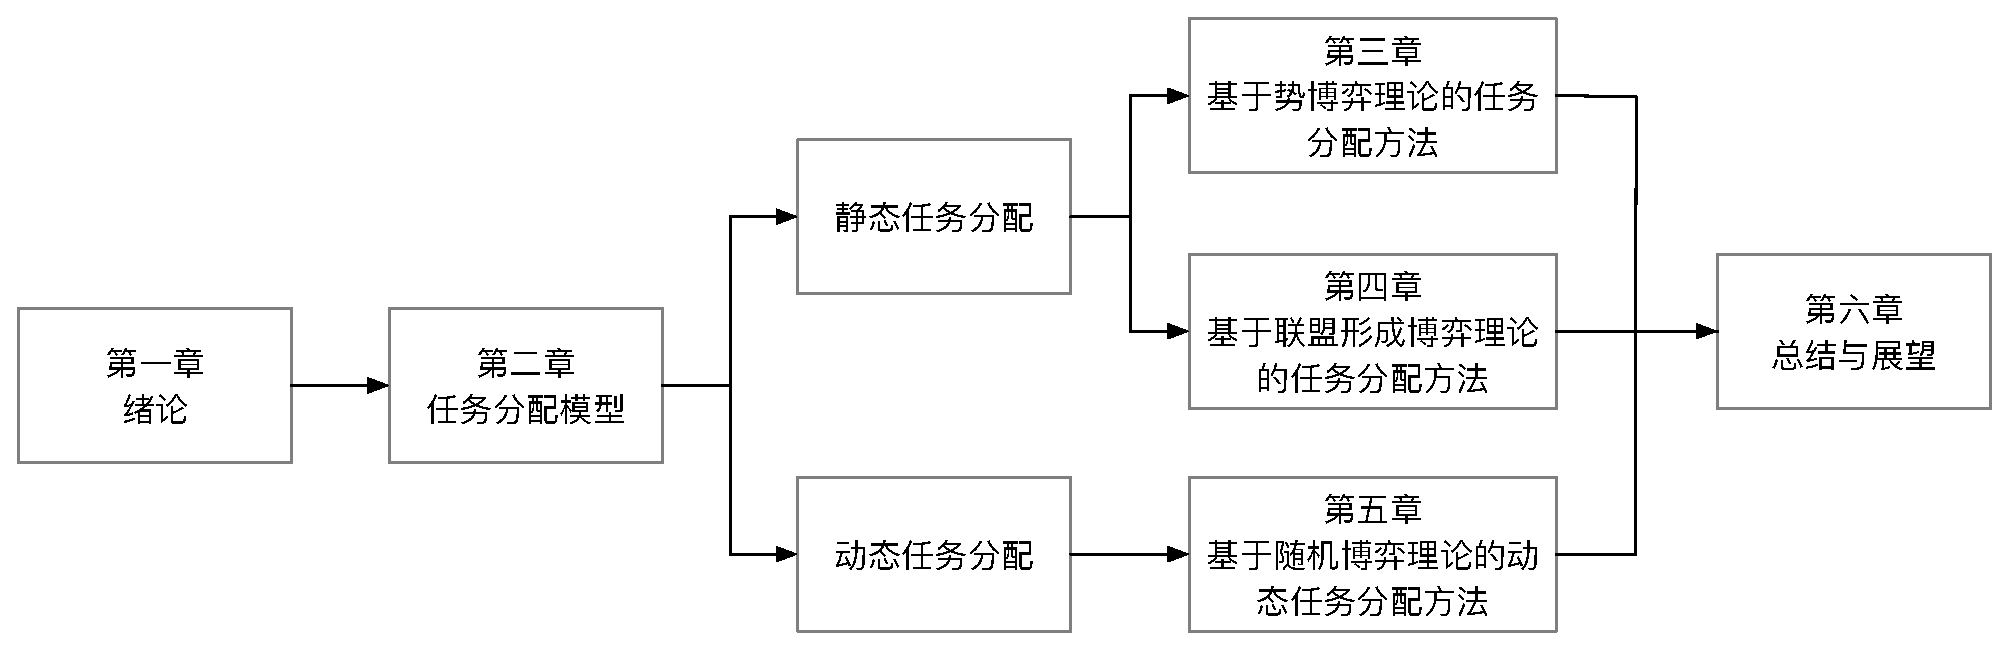
\includegraphics[height=4.5cm]{论文结构.eps} \\
  \bicaption[论文章节结构安排]
    {论文章节结构安排}
    {Structure arrangement of thesis chapters}
 \label{fig:structure}
\end{figure}

第\ref{chap:intro}章为绪论部分,首先介绍了选题背景等相关知识,简要阐述了集群空战背景下任务分配技术发展的必要性,对分布式任务分配技术的优缺点进行了归纳,并对基于博弈论思想的任务分配方法做了简要的梳理与分析,为后序博弈模型的建立和算法的设计做了铺垫。

第\ref{chap:model}章为空空导弹任务分配模型,建立了某一时间点的静态任务分配模型和一段时间的动态任务分配模型两种模型。针对静态任务分配模型,从空空导弹的特性出发,以最小化总攻击时间和最小化导弹机动量为目标,基于混合整数规划模型建立了多对多任务分配模型。针对动态任务分配模型,引入了导弹探测半径与通信半径的概念,建立了导弹对目标的探测模型以及导弹之间的通信模型,从而建立起动态场景下的任务分配模型。

第\ref{chap:pg}、\ref{chap:hedonic}章研究了针对某一时间点的分布式静态任务分配模型及其算法。

第\ref{chap:pg}章研究了基于势博弈理论的分布式任务分配方法,基于势博弈理论,基于Lagrange乘子法改进了WLU效用函数,建立了带约束条件的混合整数规划任务分配模型,通过数学推导证明了改进效用函数的有效性及性能下界。使用并比较了三种针对势博弈模型的分布式协商策略算法的有效性与性能,并改进了SAP算法,通过与集中式启发式算法的仿真对比实验,验证了设计模型与算法的有效性。

第\ref{chap:hedonic}章基于偏好联盟博弈理论,将任务分配问题看作联盟划分问题,设计了针对联盟划分问题的联盟效用函数,建立了带约束条件的偏好联盟博弈任务分配模型。从理论上推导出该模型的性能下界,得到了提高模型性能的方法。针对该模型设计了针对偏好联盟博弈模型的协商算法,改进了SAP使其适应于偏好模型,并使用DMEA算法求解。通过仿真实验验证了提出模型和算法的有效性。

第\ref{chap:stochastic}章研究了动态场景下的分布式任务分配模型及其算法。基于随机博弈理论,将导弹攻击过程划分为若干博弈子阶段,并在每个阶段建立\ref{chap:pg}、\ref{chap:hedonic}章建立的静态模型并求解。为了博弈子阶段之间的切换连贯,设计了子阶段分配前初始解的交叉生成机制和分配后新解的惰性机制。针对导弹通信网络非连通,以及目标数量发生变化两种场景进行分析并相应设计了重分配触发机制。最后通过场景仿真验证了所提出的动态分配框架的有效性,且对于动态环境有较好的应变能力。

第\ref{summary}章总结了全文的主要工作和主要贡献,并指出了本文的不足,对下一步工作也提出了展望。








% !TeX root = ../main.tex

\chapter{空空导弹任务分配模型}
\label{chap:model}

%----------------------------
\section{引言}
\label{model:sec:intro}

在任务分配问题中,首先需要根据导弹自身传感器或其他支持平台收集得到的数据和信息,估计战场态势,建立多对多的任务分配模型。在空空导弹的作战场景下,本节选择了预计剩余攻击时间和当前导弹机动量是两个较为显著且易于获得的影响要素,首先分别介绍了两个要素的估计方法,之后以最小化总攻击时间和最小化导弹机动量为目标函数,建立多对多任务分配模型。


\section{弹目相对运动模型}
\label{model:sec:move}

\begin{figure}[htp]
  \centering
  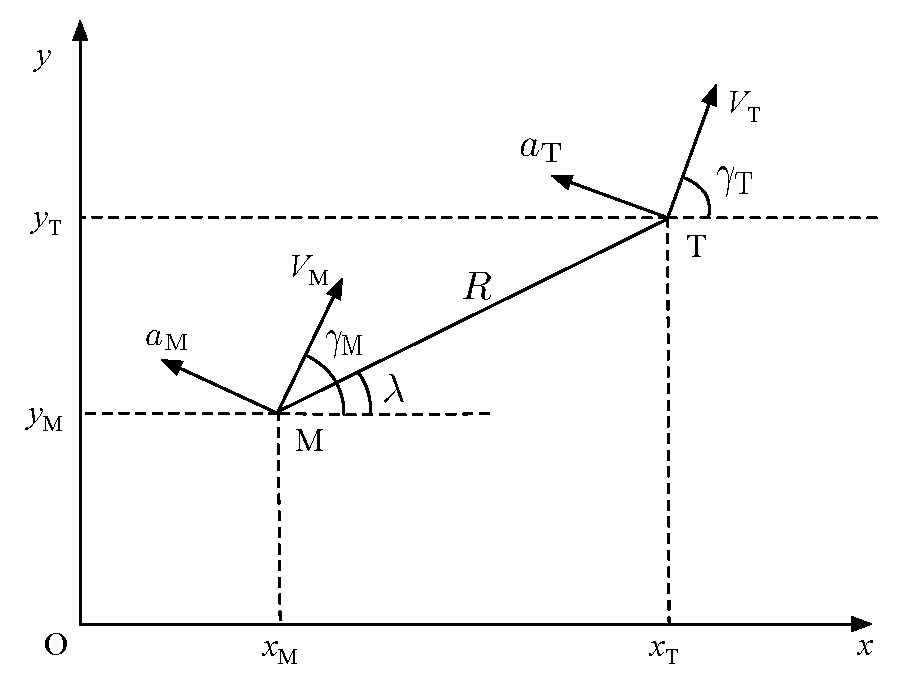
\includegraphics[width=10cm]{model.eps} \\
  \bicaption[弹目相对运动模型]
    {弹目相对运动模型}
    {Relative motion model of missile and target}
 \label{fig:model}
\end{figure}

在建立多对多任务分配模型之前,需要先建立一对一的空战模型本文所考虑的模型是在二维平面内,不考虑导弹和目标具体形状的影响,即将导弹和目标当作质点处理。图\ref{fig:model}展示的是本文所使用的导弹与目标相对运动模型,其中M表示导弹,T表示目标,$[x_{(\cdot)},y_{(\cdot)}],V_{(\cdot)},a_{(\cdot)},\gamma_{(\cdot)}$分别表示导弹和目标的位置、速度、加速度和航向角。$r$为弹目距离,$\lambda$表示弹目视线角。

为了建立弹目相对运动模型,需要作出以下假设:1、导弹与目标速度均为常值;2、目标的速度小于导弹的速度。由此分别建立导弹和目标的运动方程为:

\begin{align}
	\label{model:eq:Mmotion} \dot{x_{\text M}}&=V_{\text M} \cos{\gamma_{\text M}},\ \dot{y_{\text M}}=V_{\text M} \sin{\gamma_{\text M}},\ \dot{\gamma_{\text M}}=\dfrac{a_{\text M}}{V_{\text M}},\\
	\label{model:eq:Tmotion} \dot{x_{\text T}}&=V_{\text T} \cos{\gamma_{\text T}},\ \dot{y_{\text T}}=V_{\text T} \sin{\gamma_{\text T}},\ \dot{\gamma_{\text T}}=\dfrac{a_{\text T}}{V_{\text T}}.
\end{align}

令$V_R,V_{\lambda}$分别表示弹目相对速度平行于和垂直于视线角方向的分量,$V_R$表示弹目相对接近速度,则弹目相对运动方程为:

\begin{align}
	\label{model:eq:Rrelative} V_R & \equiv \dot{R}=V_{\text T}\cos{\sigma_{\text T}}-V_{\text M}\cos{\sigma_{\text M}},\\
	\label{model:eq:Lrelative} V_{\lambda} & \equiv R\dot{\lambda} = V_{\text T}\sin{\sigma_{\text T}}-V_{\text M}\sin{\sigma_{\text M}},
\end{align}
其中$\sigma_{(\cdot)},\ (\cdot) \in \{\text M,\text T\}$分别表示是导弹和目标的前置角,其定义为:

\begin{equation}
\label{model:eq:forwardAngle}
	\sigma_{\text M} = \gamma_{\text M}-\lambda,\quad \sigma_{\text T}=\gamma_{\text T}-\lambda.
\end{equation}

由此可求得视线角变化率:

\begin{equation}
\label{model:eq:dotlambda}
	\dot \lambda = \frac{V_{\text T}\sin{\sigma_{\text T}}-V_{\text M}\sin{\sigma_{\text M}}}{R}.
\end{equation}


% --------------------------------
\section{剩余攻击时间估计}
\label{model:sec:time}

在导弹攻击过程中,为了使得预计击中时间最短,需要估计剩余攻击时间,本节采用对目标状态投影到弹目视线方向,将目标转化为相对静止状态的思想,实现对机动目标的剩余攻击时间估计。

首先假设目标静止,即$V_{\text T}=0$。此时由式(\ref{model:eq:Mmotion})、(\ref{model:eq:forwardAngle})和(\ref{model:eq:dotlambda})可得:

\begin{equation}
\label{model:eq:dotsigma}
	\dot{\sigma_{\text M}}=\frac{a_{\text M}}{V_{\text M}}+\frac{V_{\text M}\sin{\sigma_{\text M}}}{R},
\end{equation}

结合式(\ref{model:eq:Rrelative})可得:

\begin{equation}
\label{model:eq:sigmaDotR}
	\frac{d\sigma_{\text M}}{dR} = -\frac{a_{\text M}}{V_{\text M}^2\cos{\sigma_{\text M}}}-\frac{1}{R}\tan{\sigma_{\text M}}.
\end{equation}

为方便叙述,令$\rho=\sin{\sigma_{\text M}}$,代入式(\ref{model:eq:sigmaDotR})可得:

\begin{equation}
\label{model:eq:rhoDotR}
	\frac{d\rho}{dR} = -\frac{a_{\text M}}{V_{\text M}^2}-\frac{1}{R}\rho.
\end{equation}

此处为方便推导,考虑导弹采用比例制导律,制导指令为:

\begin{equation}
\label{model:eq:png}
	a_{\text M}=N V_{\text M} \dot{\lambda},
\end{equation}
其中$N$为制导比例系数。将式(\ref{model:eq:png})和(\ref{model:eq:dotlambda})代入式(\ref{model:eq:rhoDotR})可得:

\begin{equation}
\label{model:eq:rhoDotR2}
	\frac{d\rho}{dR} = (N-1)\frac{\rho}{R}.
\end{equation}

式(\ref{model:eq:rhoDotR2})是一个一阶微分方程,其解形式为:

\begin{equation}
\label{model:eq:rho}
	\rho=\rho_0 \Bigg(\frac{R}{R_0}\Bigg)^{N-1},
\end{equation}
其中$\rho_0$和$R_0$分别为初始时刻的对应变量值。将式(\ref{model:eq:Rrelative})两边对$R$求积分,并进行泰勒展开得到:

\begin{align}
\label{model:eq:terminalTime}
	t_f &= \frac{1}{V_{\text M}} \int_0^{R_0} \frac{1}{\sqrt{1-\rho^2}}dR \notag \\
	&= \frac{1}{V_{\text M}} \int_{0}^{R_0} \Big(1+\sum_{i=1}^{\infty} \frac{2i-1}{2^i}\rho^{2i} \Big)dR,
\end{align}
其中$t_f$为初始时刻导弹已经飞行的时间。为简化问题,仅取式(\ref{model:eq:terminalTime})泰勒展开的前两项代入式(\ref{model:eq:rho})求解,并使用小角度假设$\rho \approx \sigma_{\text M}$可得:

\begin{equation}
\label{model:eq:tfsolution}
	t_f = \frac{R_0}{V_{\text M}} \Big(1+\frac{1}{2(2N-1)}\sigma_{\text M0}^2 \Big).
\end{equation}

因此,若在每个时刻均取该时刻视线角方向作为$x$轴,则可得目标静止时在每个时刻的剩余攻击时间的估计值为:

\begin{equation}
\label{model:eq:stillTF}
	t_{\text{go}} = \frac{R}{V_{\text M}} \Big(1+\frac{1}{2(2N-1)}\sigma_{\text M}^2 \Big).
\end{equation}

针对机动目标对式(\ref{model:eq:stillTF})作出进一步修正,采用虚拟目标的思路,将$V_{\text T}$和$a_{\text T}$对弹目相对运动的影响均投影到弹目视线角方向上,并修正由目标机动引起的航向角和视线角变化,将目标转化为相对静止状态。

首先得到目标机动引起的目标航向角和视线角的变化分别为:

\begin{equation}
\label{model:eq:diffsigma}
	\hat \sigma_{\text T} = \frac{a_{\text T}}{V_{\text T}}\cdot \hat t_{\text{go}}^p,\quad \hat \lambda=\frac{V_{\text T}\sin{\sigma_{\text T}}}{R}\cdot \hat t_{\text{go}}^p,
\end{equation}
其中$\hat t_{\text{go}}^p$表示前一时刻对$t_{\text{go}}$的估计值,修正后的剩余攻击时间估计为:

\begin{equation}
\label{model:eq:modifiedTF}
	\hat t_{\text {go}} = \frac{R}{V_{\text{MT}}}\Big(1+\frac{1}{2(2N-1)}\sigma_{\text M}^2 \Big)
\end{equation}
其中$V_{\text{MT}}=V_{\text M}-V_{\text T}\cos(\sigma_{\text T}+\hat \sigma_{\text T}-\lambda-\hat \lambda)$。


% --------------------------------------------
\section{能量最优制导律}
\label{model:sec:energy}

除了预计攻击时间最小化以外,由于导弹在攻击过程中大部分时间处于无动力滑翔阶段,在机动追踪目标时会不断消耗能量,因此为了保证击中目标前导弹动能不会耗尽,需要追求导弹机动程度最小化。实际中导弹系统具有高阶动态特性和非线性,难以利用最优控制原理求得闭环解,但对于只考虑导弹低阶系统特性和二次型性能指标取极小的最优控制问题,可以求得闭环解。本节将在导弹在\ref{model:sec:time}小节估计剩余攻击时间的基础上,基于最优控制原理,设计使得导弹机动最小化的最优制导律。

首先假设目标不机动,即$a_{\text T}=0$将\ref{model:sec:move}节建立的弹目相对运动模型改写为惯性系下的状态方程形式:

\begin{align}
\label{model:eq:state}
	\dot{\bm{x}} = \bm{Ax}+&\bm{Bu},\\
	\bm{A} = \begin{bmatrix}
		0 & {\bm I}_2 & 0\\
		0 & 0 & {\bm I}_2\\
		0 & 0 & -\frac{1}{\tau}{\bm I}_2\\
	\end{bmatrix},\ 
	&\bm{B} = \begin{bmatrix}
		0\\0\\\frac{1}{\tau}{\bm I}_2
	\end{bmatrix},
\end{align}
其中状态向量为${\bm x}=[{\bm R}^{\mathrm T},{\dot{\bm R}}^{\mathrm T},{\bm a}_{\text M}^{\mathrm T}]^{\mathrm T}$,各状态分量分别为对应变量的向量形式,${\bm I}_2$为二阶单位矩阵,$\tau$为导弹的等效时间常数。

设二次型的性能指标为

\begin{alignat}{2}
	\label{model:eq:J} \min \quad & J = \frac{1}{2}\int_{t_0}^{t_f} {\bm u}^{\mathrm T} {\bm u} dt,\\
	\mbox{s.t.} \quad 
	\label{model:eq:Jconstraint} & R(t_f)=0.
\end{alignat}

其中$t_0$和$t_f$分别表示制导开始和结束的时间,式(\ref{model:eq:J})可减小机动能量的消耗,有利于保持弹道平直,减小损耗增大射程。式(\ref{model:eq:Jconstraint})可约束末端脱靶量为0。

上述最优控制问题可求解闭环最优控制率形式为

\begin{equation}
\label{model:eq:closedU}
	u = ({\bm B}^{\text T}{\bm P}k^{-1})M,
\end{equation}
其中$k$是当$u=0$时的预计末端脱靶量,可由下式求得:

\begin{equation}
\label{model:eq:M}
	M={\bm P}^{\mathrm T}{\bm X}.
\end{equation}

由下列微分方程
\begin{align}
\label{model:eq:ricati}
	\dot{\bm P} + {\bm A}^{\mathrm T}{\bm P} = 0,\ {\bm P}(t_f)=\begin{bmatrix}
		1\\0\\0
	\end{bmatrix},
\end{align}
可求得$\bm P$的闭环表达式为
\begin{equation}
\label{model:eq:P}
	{\bm P} = \begin{bmatrix}
		1\\t_{\text{go}}\\\tau^2(e^{-T}+T-1)
	\end{bmatrix},
\end{equation}
其中$t_{\text{go}}$是预计剩余攻击时间,$t_{\text{go}}=t_f-t$,$T=t_{\text{go}}/\tau$。由

\begin{equation}
\label{model:eq:k}
	k = -\int_{t}^{t_f} ({\bm P}^{\mathrm T}{\bm G}{\bm G}^{\mathrm T}{\bm P}) dt,
\end{equation}
可求得$k$等于
\begin{equation}
\label{model:eq:ksolution}
	k = \tau^3(\frac{1}{2}e^{-2T} + 2Te^{-T} - \frac{T^3}{3} + T^2 - T - \frac{1}{2}).
\end{equation}

将式(\ref{model:eq:P})和式(\ref{model:eq:ksolution})代入式(\ref{model:eq:closedU})和式(\ref{model:eq:M})求得最优制导律闭合解为

\begin{equation}
\label{model:eq:oplStill}
	u = \frac{N'}{t_{\text{go}}^2} [ \bm R+\dot{\bm R}t_{\text{go}} - \tau^2(e^{-T}-1+T) {\bm a}_{\text M}],
\end{equation}
其中$N'$为扩展比例系数:

\begin{equation}
\label{model:eq:oplparameters}
	N' = T^2 (e^{-T}-{\bm I}_2+T) (-\frac{1}{2}e^{-2T} - 2Te^{-T} + \frac{1}{3}T^3 - T^2 + T + \frac{1}{2}{\bm I}_2)^{-1}.
\end{equation}

在目标机动的情况下,可对式(\ref{model:eq:oplStill})进行修正,限于篇幅,这里不再展开,直接给出对于机动目标的最优制导律:

\begin{equation}
\label{model:eq:oplMove}
	u = \frac{N'}{t_{\text{go}}^2} [ \bm R+\dot{\bm R}t_{\text{go}} - \tau^2(e^{-T}-1+T) {\bm a}_{\text M}-\frac{t_{\text{go}}^2}{2}a_{\text T}].
\end{equation}

最优性能指标$J^*$为

\begin{equation}
\label{model:eq:Jstar}
	J^* = \frac{1}{2} {\bm X}^{\mathrm T}(t_0) {\bm P}(t_0) {\bm P}^{\mathrm T}(t_0) {\bm X}(t_0).
\end{equation}

%---------------------------------------------
\section{任务分配模型建立}
\label{model:sec:assignment}

\subsection{基本模型}
\label{model:basic_model}

假设我方有$n_m$枚导弹,其集合表示为$\mathcal{M} := \{\mathcal{M}_1,\dots,\mathcal{M}_{n_v}\}$;战场上有$n_t$个目标需要攻击,其集合表示为$\mathcal{T} := \{\mathcal{T}_0,\mathcal{T}_1,\dots,\mathcal{T}_{n_t}\}$,其中$\mathcal{T}_0$表示空目标。本文只考虑导弹数量不少于目标数量,即$n_m \geq n_t$的情况。每枚导弹可根据自身能力、所处环境等因素选择部分目标作为可攻击对象,设$\mathcal{A}_i \subset \mathcal{T}$表示第$i$枚导弹的可选目标集。特别地,为后续叙述方便,假设$\mathcal{T}_0 \in \mathcal{A}_i,\ i=1,\dots,n_m$,即所有导弹总是可以选择不攻击任何目标。\footnote{显然,根据实际场景以及约束条件可知导弹不攻击任何目标是不符合实际要求的,本文在此作出的假设仅仅是为了后面章节叙述和论证需要,无任何实际意义,对问题的论述和求解也无任何影响。}导弹$i$从自己的可选目标集$\mathcal{A}_i$中选出自己的目标$a_i$,则数组$a=(a_1,\dots,a_{n_m})\in \mathcal{A}$组成了一个分配解。设$S(a)=\{S_1,\dots,S_{n_t}\}$,其中$S_j$表示分配解$a$下选择目标$j$的导弹集合,$s_j$表示$S_j$中的导弹个数,即$s_j = |S_j|, j=1,\dots,n_t$。

选取一个关于分配解$a$的函数$U_g(a)$作为全局效用函数,建立任务分配模型:

\begin{alignat}{2}
	\label{model:eq:globalU} \max_{a \in \mathcal{A}} \quad & U_g(a) = \sum_{\mathcal{T}_j \in \mathcal{T}} U_{\mathcal T_j}(a)\\
	\mbox{s.t.} \quad 
	\label{model:eq:bmax} & s_j \leq b_{\text{max}}^{(j)},\ j=1,\dots,n_t\\
	\label{model:eq:bmin}& s_j \geq 1,\ j=1,\dots,n_t,
\end{alignat}
其中$b_{\text{max}}^{(j)}$表示选择目标$j$的导弹的最大数量和最小数量,且有$b_{\text{max}}^{(j)} \geq 1$。因此式(\ref{model:eq:bmax})表示目标$j$不得被超过$b_{\text{max}}^{(j)}$枚导弹攻击,式(\ref{model:eq:bmin})代表每个目标必须有导弹攻击,但由于实际中往往使用多于目标数量的导弹攻击,因此在式(\ref{model:eq:bmin})的约束下,式(\ref{model:eq:bmin})自然成立,因此可将上述问题进一步简化为

\begin{alignat}{2}
	\label{model:eq:simUg} \max_{a \in \mathcal{A}} \quad & U_g(a) = \sum_{\mathcal{T}_j \in \mathcal{T}} U_{\mathcal T_j}(a)\\
	\mbox{s.t.} \quad 
	\label{model:eq:simbmax} & s_j \leq b_{\text{max}}^{(j)},\ j=1,\dots,n_t.
\end{alignat}

$U_{\mathcal T_j}(a)$表示与目标$\mathcal{T}_j$有关的任务效用,为了体现预计剩余攻击时间最小和导弹机动能量消耗最小的目标,利用\ref{model:sec:time}小节和\ref{model:sec:energy}小节的内容,将任务效用函数设计为:

\begin{equation}
\label{model:eq:taskU}
	U_{\mathcal{T}_j}(a) = r_j - \sum_{\mathcal{M}_i \in S_j} c_{ij},
\end{equation}
其中,$r_j$是目标$\mathcal{T}_j$的价值,本文假设该值仅与目标属性有关,与攻击的导弹无关;$x_{ij}$表示导弹$\mathcal{M}_i$攻击目标$\mathcal{T}_j$的成本函数,其定义为

\begin{equation}
\label{model:eq:cost}
	c_{ij} = w_1 t_{ij} + w_2 \mathcal{J}_{ij},
\end{equation}
其中,$w_1$和$w_2$为权重值,代表对于攻击时间和攻击消耗能量的权衡程度;$t_{ij}$表示导弹$\mathcal{M}_i$攻击目标$\mathcal{T}_j$的预计剩余攻击时间。$J_{ij}$为导弹$\mathcal{M}_i$攻击目标$\mathcal{T}_j$的预计机动能量消耗可由式(\ref{model:eq:Jstar})得到。

\subsection{动态任务分配模型}
\label{model:dynamic_model}

前一小节所介绍的基本任务分配模型只是用于某一静止时间点或短期时间内的任务分配模型,为了研究在高度动态的空战模型中的任务分配问题,本节建立了分布式的动态任务分配模型。本节从导弹对目标的探测和导弹之间的通信入手建立模型。

在实际战场上,导弹发射之前往往是由地面雷达或载机雷达提供目标信息,因此本文假设导弹在发射前已知所有目标信息且全局共享。但在导弹发射后,需要单纯依靠导弹之间通信进行目标的探测、跟踪和分配,地面雷达或载机不再提供目标新的信息。对目标的探测与跟踪并不是本文的重点,因此本文不再展开,且不考虑目标存在发射干扰弹等逃脱行为,则将该问题简化为只要目标在导弹的探测范围内即可认为导弹实现了对目标的探测和跟踪。

对于导弹之间的通信,本文假设导弹的通信方式为广播式,且广播通信半径有限,即在通信半径内的导弹可实现双向通信。为简化问题,本文中的通信不考虑时延、丢包、噪声等问题,即导弹之间的通信是双向且即时可靠的,因此导弹之间的通信网络可用一个无向图表示,在该无向图中,用节点表示导弹,用边表示直接通信通道。另外,在实际中,导弹之间即使没有建立起直接通道,也可以通过其他导弹进行通信路由,实现信息的传输,因此本文认为两节点间只要存在路径,这两个节点便可实现信息交互。

\begin{figure}[!htp]
  \centering
  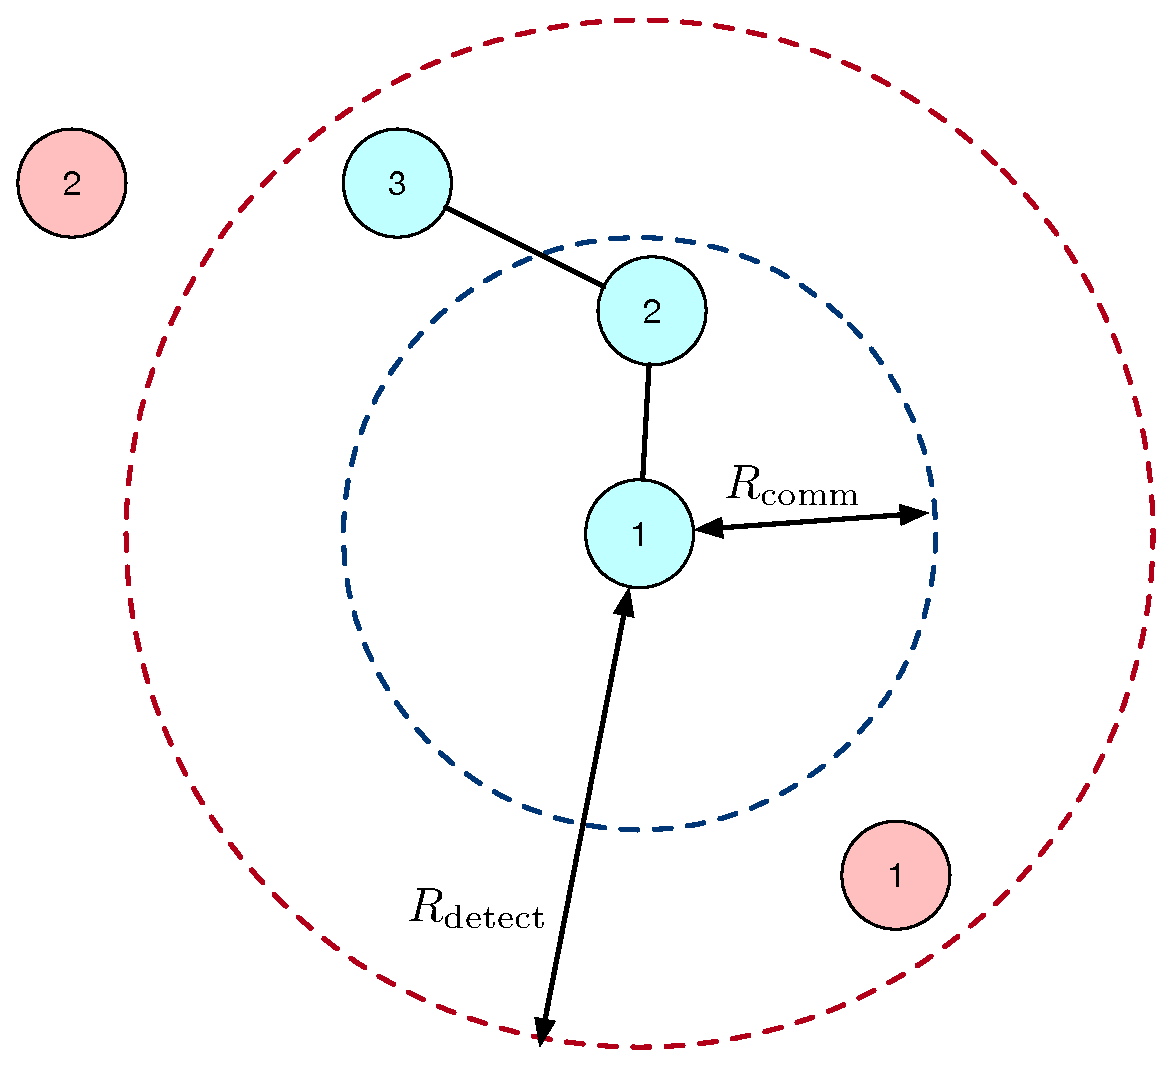
\includegraphics[height=7cm]{半径模型.eps}
  \bicaption[导弹探测与通信示意图]
    {导弹探测与通信示意图}
    {Diagram of detection and communication of missiles}
  \label{fig:detect_and_com}
\end{figure}

用图\ref{fig:detect_and_com}详细解释本文的假设,图中用蓝色节点代表导弹,红色节点代表目标,红色虚线圈代表导弹的探测范围,蓝色虚线圈代表导弹的通信范围,$R_{\text{detect}}$和$R_{\text{comm}}$分别代表导弹的探测半径和通信半径\footnote{为方便展示在图中将导弹和目标均用圆圈表示,在本文实际建立的模型中将导弹和目标均看作质点,没有大小和半径}。由于导弹2位于导弹1的通信范围内,因此导弹1和导弹2之间建立了通信通道,而导弹3超出了导弹1的通信范围,因此导弹1和3之间没有直接的通信通道,但导弹2和3之间也有一条通道。目标1位于导弹1的探测范围内,因此导弹1可以知晓目标1的相关信息,由于信息交互的假设,导弹2和3均可通过交互得到目标1的信息;与此同时,虽然目标2不在导弹1的探测范围内,但由于目标2位于导弹3的探测范围内,导弹1仍可间接通过导弹3获知目标2的信息。


\section{本章小结}
\label{model:sec:conclusion}
本章基于攻击时间最小化和导弹机动消耗最小化的原则建立了空空导弹任务分配模型。首先建立了弹目相对运动模型,对导弹和目标的运动方程进行建模。接着基于该相对运动模型估计剩余攻击时间,并设计导弹遵循最优制导律飞行已获得最小机动消耗。接着,本章定义了全局效用函数和任务效用函数的概念,建立了导弹与目标的静态任务分配模型;最后,本文引入了导弹对目标的探测模型和导弹之间的通信模型与假设,建立了动态环境下的任务分配模型,为后续求解空空导弹的任务分配问题打下基础。















% !TEX root = ../main.tex

\chapter{基于势博弈模型的分布式任务分配}
\label{chap:pg}



\section{引言}
\label{pg:intro}

本章使用第\ref{chap:model}章中建立的空空导弹任务分配模型,设计了面向任务分配问题的势博弈模型(Potential Game, PG)框架。本章首先介绍了势博弈模型概念,并选择合适的函数作为智能体效用,初步建立了势博弈模型;接着针对任务分配中的约束问题,使用Lagrange乘子法对原始势博弈模型进行改进,并证明了模型的可行性与性能下界;然后,针对改进的势博弈模型,使用多种均衡求解算法进行模型求解;最后,通过仿真与对比实验验证了模型与算法的有效性。

%--------------------------------
%--------------------------------
\section{势博弈模型}
\label{pg:model}
在任务分配问题框架下,当所有导弹依据最大化自身效用的原则选择的目标不再发生变化时,则称所有导弹达到了均衡状态。博弈论中一个经典的均衡状态是纯纳什均衡,它表示一个任务分配解$a^*=(a_1^*,\dots,a_{n_m}^*)$,满足任意一个导弹不能通过独自改变任务提高自身效用。在具体阐述纳什均衡和势博弈概念前,除第\ref{chap:model}章使用的概念外,仍需要引入以下概念和符号。设$a_{-i}$表示除了导弹$\mathcal{M}_i$以外的其他导弹的分配集合,即
\[
a_{-i}=(a_1,\dots,a_{i-1},a_{i+1},\dots,a_{n_m}),
\]
利用该符号可将一组分配解表示为$(a_i,a_{-i})$。此外,可类似地定义$\mathcal{A}_{-i}$为
\[
\mathcal{A}_i:=\mathcal{A}_1 \times \dots \times \mathcal{A}_{i-1} \times \mathcal{A}_{i+1} \times \dots \times \mathcal{A}_{n_m} .
\]
设$U_{\mathcal{M}_i}(a)$或$U_{\mathcal{M}_i}(a_i,a_{-i})$表示导弹$\mathcal{M}_i$在分配$a$下的智能体效用,由此可得到纯纳什均衡的定义:
\begin{definition}[纯纳什均衡]
\label{pg:def:pureNash}
	若一个分配解$a^*$满足
	\begin{equation}
\label{pg:eq:pure_Nash}
	U_{\mathcal{M}_i}(a_i^*,a_{-i}^*)=\max_{a_i\in \mathcal{A}_i}U_{\mathcal{M}_i}(a_i,a_{-i}^*),\quad \forall \mathcal{M}_i \in \mathcal{M}.
\end{equation}
则称$a^*$是一个纯纳什均衡解。
\end{definition}

当所有导弹达到纯纳什均衡时,全局效用未必实现最大化;另一方面,在一些博弈场景下纯纳什均衡未必存在。因此,引入势博弈概念

\begin{definition}[有序势博弈与势博弈]
\label{pg:def:potentialGame}
	设一个博弈模型中的智能体效用函数为$U_{\mathcal{M}_i}(a),\mathcal{M}_i\in \mathcal{M}$,如果存在一个全局势函数$\phi(a):\mathcal{A} \mapsto \mathbb{R}$,满足对任意智能体$\mathcal{M}_i \in \mathcal{M}$,任意$a_{-i}\in \mathcal{A}_{-i}$,智能体$\mathcal{M}_i$的任意两个分配$a_i',a_i''\in \mathcal{A}_i$,有
	\begin{equation}
	\label{pg:eq:ordpg}
		U_{\mathcal{M}_i}(a_i',a_{-i})-U_{\mathcal{M}_i}(a_i'',a_{-i})>0 \Leftrightarrow \phi(a_i',a_{-i})-\phi(a_i'',a_{-i})>0,
	\end{equation}
	则该博弈模型是一个有序势博弈模型。在此基础上,若该全局势函数进一步满足:
	
	\begin{equation}
	\label{pg:eq:pgdef}
		U_{\mathcal{M}_i}(a_i',a_{-i})-U_{\mathcal{M}_i}(a_i'',a_{-i})=\phi(a_i',a_{-i})-\phi(a_i'',a_{-i}).
	\end{equation}
	则称该博弈模型为势博弈模型。若策略集$\mathcal{A}$是有限的,则称该势博弈为有限势博弈。
\end{definition}

由势博弈的定义可知,势博弈模型中的智能体效用变化会等同地反映在全局效用上,而在有序势博弈上,智能体效用与全局效用总是同向变化。易知势博弈是一种特殊的有序势博弈。有限势博弈模型有两点性质:

(1)有限势博弈至少存在一个纯纳什均衡;

(2)有限势博弈具有有限优化性质(finite improvement property, FIP)。

性质(1)保证了纯纳什均衡的存在性,因此对于任务分配问题,至少可以得到一个确定的解;性质(2)保证了任意智能体单方面提高自己效用的行为可以在有限时间内收敛到纯纳什均衡,从而保证了优化算法可在有限时间内收敛。




%--------------------------------
%--------------------------------
%-------------------------------------------------
%-----------------------------------------------

%--------------------------------
\section{智能体效用函数}
\label{pg:wlu}


使用势博弈模型解决任务分配问题对导弹的智能体效用函数提出的要求是,满足

\begin{equation}
\label{pg:eq:pgU}
	U_{\mathcal{M}_i}(a_i',a_{-i})-U_{\mathcal{M}_i}(a_i'',a_{-i})=U_g(a_i',a_{-i})-U_g(a_i'',a_{-i}),
\end{equation}
使得所有导弹形成一个势博弈模型,其中$U_g(a)$即为式(\ref{model:eq:globalU})中定义的全局效用函数,因此在求解分配时所有导弹只需考虑最大化智能体效用便可实现全局效用最大化的目标。

一个显然而直接的思路是使用一致利益效用(Identical Interest Utility, IIU),其直接将全局效用作为智能体效用,但IIU的缺点在于需要计算所有任务效用后得到全局效用,因此本质上仍是集中式的方法。对IIU进行改进可以得到更分布化的有限区域效用(Range-Restricted Utility, RRU),RRU将智能体效用定义为所有该智能体参与的任务的效用之和,RRU可以使得智能体组成势博弈模型,但该模型的纳什均衡未必是最优的。此外,IIU和RRU有一个共同的问题在于如果存在大量的智能体同时参与大量的任务,由于IIU和RRU都是对一定数量的任务效用求和,此时一个智能体对任务的贡献微乎其微,即使它单方面改变决策,对该任务的效用改变可能很小,从而反映在智能体效用函数上的变化也很小。这对智能体的寻优和学习带来了很大难度。对此问题作出的改进是等份额效用(Equally Shared Utility, ESU),ESU用智能体参与的任务效用除以参与该任务的智能体总数,可以有效消除智能体数量带来的效用稀释作用,但ESU的局限在于只有当智能体之间不存在区别时才可以组成势博弈模型。

为了克服IIU和RRU的缺陷,且不局限于ESU的应用场景,本节采用的是美好生活效用函数(Wonderful Life Utility, WLU),WLU将智能体效用函数定义为每个智能体对全局效用的边际贡献程度,其具体定义为:

\begin{equation}
\label{pg:eq:WLU1}
	U_{\mathcal{M}_i}(a_i,a_{-i}) = U_g(a_i,a_{-i}) - U_g(a_0,a_{-i}).
\end{equation}

由全局效用函数的定义式(\ref{model:eq:globalU})可将式(\ref{pg:eq:WLU1})改写为

\begin{equation}
\label{pg:eq:WLU2}
	U_{\mathcal{M}_i}(a_i,a_{-i}) = U_{\mathcal{T}_j}(a_i,a_{-i}) - U_{\mathcal{T}_j}(a_0,a_{-i}),\quad \text{if}\ a_i=\mathcal{T}_j.
\end{equation}

由式(\ref{pg:eq:WLU2})可知,WLU假设其他智能体不改变目标,智能体效用只与智能体自身的决策有关,因此WLU排除了冗余信息,比IIU和RRU优化能力更强。另外,下面的命题表明,使用WLU的博弈模型一定是势博弈模型。

\begin{proposition}[WLU可行性]
\label{pg:pro:mwlu}
	智能体效用函数为式(\ref{pg:eq:WLU2})的智能体集合组成的博弈模型是一个势博弈模型,且其势函数就是全局效用函数$U_g(a)$。
	
	\begin{proof}
	只需证明WLU满足式(\ref{pg:eq:pgU})即可。设$a_i,a_i' \in \mathcal{A}_i$,则有
	\begin{align}
		&\ U_{\mathcal{M}_i}(a_i,a_{-i}) - U_{\mathcal{M}_i}(a_i',a_{-i})\notag\\
		=&\ U_g(a_i,a_{-i}) - U_g(a_0,a_{-i}) - [U_g(a_i',a_{-i}) - U_g(a_0,a_{-i})]\notag\\
		=&\ U_g(a_i,a_{-i}) - U_g(a_i',a_{-i}) \notag
	\end{align}
	\end{proof}
\end{proposition}



\section{约束条件处理方法}
\label{pg:mwlu}

上述势博弈框架和智能体效用函数设计下,对于智能体选择任务并没有做出任何限制和约束,因此需要利用约束条件式(\ref{model:eq:simbmax})将势博弈的纳什均衡限制在可行解中。本节提出了基于Lagrange乘子法将有约束问题转化为无约束问题,并证明了在满足一定的条件下,新的无约束问题下获得的纳什均衡解均为原问题的可行解。

Lagrange乘子法是一种典型的处理含约束优化问题的方法,其将含约束问题转化为无约束问题,且可证明生成的新的无约束问题的最优解就是原问题的最优解。在势博弈模型下,结合全局效用函数的定义式(\ref{model:eq:simUg})以及约束条件式(\ref{model:eq:bmax}),将式(\ref{model:eq:taskU})任务效用函数$U_{\mathcal{T}_i}(a)$修正为:

\begin{equation}
\label{pg:eq:newTaskU}
	\widetilde U_{\mathcal{T}_j}(a) = U_{\mathcal{T}_j}(a) + \lambda [b_{\text{max}}^{(j)} - s_j]^-,
\end{equation}
其中$[x]^+=\min\{x,0\}$,$s_j$是第二章中定义的目标同为$\mathcal{T}_j$的导弹数量。由式(\ref{model:eq:globalU})得到修正后的全局效用函数为

\begin{equation}
\label{pg:eq:newglobalU}
		\widetilde U_g(a) = U_g(a) +  \lambda \sum_{j=1}^{n_t}[b_{\text{max}}^{(j)} - s_j]^-
	\end{equation}

再利用式(\ref{pg:eq:WLU2})提出的WLU效用函数计算修正后的智能体效用函数(Modified WLU, MWLU)为

\begin{align}
\label{pg:eq:newAgentU}
	\widetilde U_{\mathcal{M}_i}(a_i,a_{-i}) &= \widetilde U_g(a_i,a_{-i}) - \widetilde U_g(a_0,a_{-i})\notag\\
	&= \widetilde U_{\mathcal{T}_j}(a_i,a_{-i}) - \widetilde U_{\mathcal{T}_j}(a_0,a_{-i}),\quad \text{if}\ a_i=\mathcal{T}_j.
\end{align}

下面需要验证MWLU的有效性,主要分为三部分:(1)满足MWLU效用的智能体能否组成势博弈模型;(2)该势博弈模型下得到的纳什均衡是否都满足原问题的约束;(3)该势博弈模型下得到的纳什均衡解的最优性。

%----------------------------
\subsection{势博弈成立条件}
\label{pg:mwlu:pgcondition}
为了验证MWLU函数的有效性,首先需要验证式(\ref{pg:eq:newAgentU})定义的智能体效用函数是否可以组成一个势博弈模型。设智能体效用函数为MWLU的智能体组成的组成的博弈模型为$\mathcal{G}=\{\mathcal{M},\mathcal{A},U_{\mathcal{M}}(a)\}$,实际上,可以得到以下结论:

\begin{proposition}[势博弈成立条件]
	$\mathcal{G}$是一个势博弈模型,其势函数为式(\ref{pg:eq:newglobalU})定义的全局效用函数。
	
	\begin{proof}
		只需证明全局效用函数$\widetilde U_g(a)$与式(\ref{pg:eq:newAgentU})定义的智能体效用函数$\widetilde U_{\mathcal{M}_i}(a_i,a_{-i})$满足式(\ref{pg:eq:pgU})即可。对任意$a_i',a_i'' \in \mathcal{A}_i$,$a'=(a_i',a_{-i}),a''=(a_i'',a_{-i})$,且$S',S''$分别为$a'$和$a''$对应的智能体分配集合,$s_j'$和$s_j''$分别为$S'$和$S''$中目标为$\mathcal{T}_j$的智能体数量。假设$a_i'=\mathcal{T}_j,\ a_i''=\mathcal{T}_k,\ j\neq k$,则有
		\begin{align}
			&\widetilde U_{\mathcal{M}_i}(a_i',a_{-i}) - \widetilde U_{\mathcal{M}_i}(a_i'',a_{-i})\notag\\
			= &\ [\widetilde U_g(a_i',a_{-i}) - \widetilde U_g(a_0,a_{-i})] - [\widetilde U_g(a_i'',a_{-i}) - \widetilde U_g(a_0,a_{-i})]\notag\\
			\label{pg:pf:eq:pg} = &\ \widetilde U_g(a_i',a_{-i}) - \widetilde U_g(a_i'',a_{-i})
		\end{align}
		所以满足MWLU效用的智能体可以组成一个势博弈模型,且势函数为全局效用函数$\widetilde U_g(a)$。
	\end{proof}
\end{proposition}

%--------------------------------
\subsection{纯纳什均衡可行性分析}
\label{pg:mwlu:pgexist}
在验证势博弈模型成立之后,下一步需要验证该势博弈模型所得到的纯纳什均衡是否是原问题的可行解,此处有以下结论:

\begin{proposition}[纳什均衡可行性]
\label{pg:pro:feasibility}
	当$\lambda$满足$\lambda > \lambda_0$时,若分配策略$a$是$\mathcal{G}$的一个纯纳什均衡,则$a$一定满足约束条件(\ref{model:eq:bmax})。其中
	\begin{equation}
		\lambda_0 = \max_{\substack{\mathcal{M}_i \in \mathcal{M}, \mathcal{T}_j \in \mathcal{T} \\ s_j > b_{\text{max}}^{(j)}}} \Bigg\{ \frac{U_{\mathcal{T}_j}(a_i,a_{-i}) - U_{\mathcal{T}_j}(a_i',a_{-i})}{s_j-b_{\text{max}}^{(j)}} \Bigg\}
	\end{equation}
	
	\begin{proof}
		设$a^*=(a_i^*,a_{-i}^*)$是势博弈模型$\mathcal{G}$的一个纯纳什均衡,但不满足约束条件(\ref{model:eq:bmax}),即存在$1\leq j \leq n_t, s_j^* > b_{\text{max}}^{(j)}$。对于参与任务$\mathcal{T}_j$的智能体之一$\mathcal{M}_k$,设$a_k^*=\mathcal{T}_j,a_k'=\mathcal{T}_l,\forall l \neq j$,则有
		\begin{align}
			&\widetilde U_{\mathcal{M}_k}(a_k^*,a_{-k}^*) - \widetilde U_{\mathcal{M}_k}(a_k',a_{-k}^*)\notag\\
		    =&\ \widetilde U_{\mathcal{T}_j}(a_k^*,a_{-k}^*) - \widetilde U_{\mathcal{T}_l}(a_k',a_{-k}^*)\notag\\
		    =&\ U_{\mathcal{T}_j}(a_k^*,a_{-k}^*) - \lambda(s_j^*-b_{\text{max}}^{(j)}) - [U_{\mathcal{T}_l}(a_k',a_{-k}^*) + \lambda[b_{\text{max}}^{(l)} - s_l']^-]\notag\\
		    \leq &\ U_{\mathcal{T}_j}(a_k^*,a_{-k}^*) - U_{\mathcal{T}_l}(a_k',a_{-k}^*) - \lambda(s_j^*-b_{\text{max}}^{(j)}) \notag \\
		    \leq &\ \max_{\mathcal{T}_j \in \mathcal{T}} \{U_{\mathcal{T}_j}(a_i^*,a_{-i}^*) - U_{\mathcal{T}_j}(a_i',a_{-i}^*)\} - \lambda_0(s_j^*-b_{\text{max}}^{(j)})
		\end{align}
		由$\lambda_0$的定义易知$\widetilde U_{\mathcal{M}_{k_0}}(a_{k_0}^*,a_{-{k_0}}^*) - \widetilde U_{\mathcal{M}_{k_0}}(a_{k_0}',a_{-{k_0}}^*) \leq 0$,这与$a^*$是纯纳什均衡的条件(\ref{pg:eq:pure_Nash})矛盾,因此$a^*$必然满足约束条件。
	\end{proof}
	
\end{proposition}

%---------------------
\subsection{纳什均衡最优性}
\label{pg:mwlu:pgoptimal}

在命题\ref{pg:pro:feasibility}下,势博弈模型$\mathcal{G}$的纳什均衡均为原问题的可行解,因此最后需要考察这些纳什均衡解的最优性。本节选择使用无秩序代价(Price of Anarchy, PoA)作为衡量纳什均衡性能的指标。设纯纳什均衡分配解为$a^*$,全局最优分配解为$a^{\text{opt}}$,则PoA的定义为全局最优效用和纳什均衡效用的最小值之比:
\begin{equation}
\label{pg:eq:PoA}
	\mathrm{PoA}(\mathcal{G}) = \frac{U_g(a^{\text{opt}})}{\min_{a^*} U_g(a^*)}
\end{equation}

由PoA的定义可知,PoA越大,代表最差情况下纯纳什均衡效用越小,即意味着该势博弈模型的性能越差。关于本节建立的势博弈模型$\mathcal{G}$的PoA,我们可以用以下命题得到PoA的上界,从而保证了势博弈模型性能的下界。

\begin{proposition}
\label{pg:pro:PoA}
	势博弈模型$\mathcal{G}$的PoA上界为
	\begin{equation}
	\label{pg:pro:eq:High_Bound_PoA}
		\mathrm{PoA}(\mathcal{G}) \leq 1 + \eta
	\end{equation}
	其中
	\begin{equation}
	\label{pg:pro:eq:eta_PoA}
		\eta= \max_{\substack{\forall a,a' \in \mathcal{A}\\ \forall \mathcal{M}_i \in \mathcal{M}}} \Bigg\{ \frac{\widetilde U_g(a') - \widetilde U_g(a_i',a_{-i})}{\widetilde U_g(a)} \Bigg\}
	\end{equation}
	
	\begin{proof}
		设$a^{\text{opt}}$是全局最优分配解,$a^*$是一纯纳什均衡分配解。由纯纳什均衡的定义式(\ref{pg:eq:pure_Nash})可得
		\begin{equation}
		\label{pg:pro:eq:inequality_Um}
			\widetilde U_{\mathcal{M}_i}(a_i^*,a_{-i}^*) \geq \widetilde U_{\mathcal{M}_i}(a_i^{\text{opt}},a_{-i}^*),\ \forall \mathcal{M}_i \in \mathcal{M}.
		\end{equation}
		将式(\ref{pg:eq:pgU})代入可得
		\begin{equation}
		\label{pg:pro:eq:inequality_Ug}
			\widetilde U_g(a_i^*,a_{-i}^*) \geq \widetilde U_g(a_i^{\text{opt}},a_{-i}^*).
		\end{equation}
		
		不等式右侧可以写为
		\begin{equation}
		\label{pg:pro:eq:rewrite}
			\widetilde U_g(a_i^{\text{opt}},a_{-i}^*) = \widetilde U_g(a_i^{\text{opt}},a_{-i}^{\text{opt}}) - [\widetilde U_g(a_i^{\text{opt}},a_{-i}^{\text{opt}}) - \widetilde U_g(a_i^{\text{opt}},a_{-i}^*)],
		\end{equation}
		所以有
		\begin{equation}
		\label{pg:pro:eq:relation_opt_nash}
			\widetilde U_g(a^*) \geq \widetilde U_g(a^{\text{opt}}) - [\widetilde U_g(a^{\text{opt}}) - \widetilde U_g(a_i^{\text{opt}},a_{-i}^*)],
		\end{equation}
		两边同时除以$\widetilde U_g(a^*)$,
		\begin{align}
		\label{pg:pro:eq:cal_PoA}
			\frac{U_g(a^{\text{opt}})}{U_g(a^*)} &\leq 1 + \frac{\widetilde U_g(a^{\text{opt}}) - \widetilde U_g(a_i^{\text{opt}},a_{-i}^*)}{\widetilde U_g(a^*)}\notag\\
			&\leq 1 + \max_{\substack{\forall a,a' \in \mathcal{A}\\ \forall \mathcal{M}_i \in \mathcal{M}}} \Bigg\{ \frac{\widetilde U_g(a') - \widetilde U_g(a_i',a_{-i})}{\widetilde U_g(a)} \Bigg\}\notag\\
			&\triangleq 1 +\eta
		\end{align}
		
		因此
		\begin{equation}
		\label{pg:pro:eq:comclusion_PoA}
			\mathrm{PoA}(\mathcal{G}) \leq 1 + \eta
		\end{equation}
	\end{proof}
\end{proposition}


%----------------------------------------
\section{均衡求解}
\label{pg:pgta:protocal}

\subsection{虚拟博弈算法}
\label{pgta:protocal:FP}
虚拟博弈算法(Fictitious Play, FP)是一种经典的学习算法,最初被用来求解零和博弈中的纳什均衡,但也被提出可以用于多智能体系统的学习算法。在本节,虚拟博弈算法被视为智能体选择目标的机制。在每个时刻$k$,智能体$i$计算自身的经验频率分布$q_i(k)$,并根据该分布选择下一步最优决策。智能体经验频率分布定义为

\begin{equation}
\label{pg:eq:frequency}
	q_i^j(k) = \frac{1}{k} \sum_{t=0}^{k-1} I\{a_i = A_i^j\},\ A_i^j \in \mathcal{A}_i, j = 1,\dots,|\mathcal{A}_i|,
\end{equation}
其中$I\{\cdot\}$为指示函数,$|\mathcal{A}_i|$表示目标集$\mathcal{A}_i$的势。

智能体$i$在FP下选择目标的策略是假设其他智能体会独立地根据各自的经验频率分布随机选择一个目标。在此假设下,可计算出智能体$i$选择目标$A_i^j$的期望效用为

\begin{align}
\label{pg:eq:expectU}
	U_i(A_i^j, q_{-i}(k)) &= \mathbb{E}_{a_{-i}}[U_{\mathcal{M}_i}(A_i^j,a_{-i})]\notag\\
	&= \sum_{a_{-i}\in \mathcal{A}_{-i}} U_{\mathcal{M}_i}(A_i^j, a_{-i}) \prod_{a_j \in \mathcal{A}_{-i}} q_j^{a_j}(k),
\end{align}
其中$q_{-i}(k):=\{q_1(k),\dots,q_{i-1}(k),q_{i+1}(k),\dots,q_{n_m}(k)\}$。因此,智能体$i$在$k$时刻选择的最优目标$a_i(k)$为
\begin{equation}
\label{pg:eq:bestResponse}
	a_i(k) \in \arg \max_{\alpha \in \mathcal{A}_i} U_i(a, q_{-i}(k)),
\end{equation}
若同时存在多个最优目标,则在多个最优目标中任选一个。

FP的优点在于除了极少数特殊情况,根据经验频率分布选出的目标分配解几乎都会收敛到纳什均衡。但FP的缺点也是显然的,每个智能体在作出决策时需要知道所有智能体的经验频率分布,且计算出所有组合情况下的效用的期望,因此FP的计算时间和计算复杂度会随着智能体数量的增加而急剧增加。

为了提高FP的可行性,联合策略虚拟博弈(Joint Strategy Fictitious Play, JSFP)在FP的基础上做出了改进。JSFP最主要的改进在于在计算不同目标选择的效用时,取消了其他智能体选择目标的独立性条件,从而在计算经验频率分布时,计算的是一个分配组合$a$的经验频率而不是某个特定目标的频率。在JSFP下,联合经验频率$z(\overline a,k)$的计算公式为

\begin{equation}
\label{pg:eq:jsef}
	z(\overline a,k) = \frac{1}{k} \sum_{t=0}^{k-1} I\{a(k) = \overline a\},\quad \overline a \in \mathcal{A},
\end{equation}
类似地可定义出$z_{-i}(\overline a,k)$的定义为

\begin{equation}
\label{pg:eq:jsefForMinusi}
	z_{-i}(\overline a_{-i},k) = \frac{1}{k} \sum_{t=0}^{k-1} I\{a_{-i}(k) = \overline a_{-i}\},\quad \overline a \in \mathcal{A}.
\end{equation}

因此此时智能体$i$选择目标$\overline a_i$的期望效用是

\begin{equation}
\label{pg:eq:jsfpExpectU}
	U_i(\overline a_i,k) = \sum_{a_{-i} \in \mathcal{A}_{-i}} U_{\mathcal{M}_i}(\overline a_i,a_{-i}) z_{-i}(\overline a_{-i},k)
\end{equation}

JSFP第二个改进的地方在于,虽然式(\ref{pg:eq:jsfpExpectU})似乎仍需要计算所有组合策略情况下的期望,但通过将式(\ref{pg:eq:jsefForMinusi})代入式(\ref{pg:eq:jsfpExpectU})可得

\begin{equation}
\label{pg:eq:modifiedEU}
	U_i(\overline a_i, z_{-i}(k)) = \frac{1}{k}\sum_{t=0}^{k-1} U_{\mathcal{M}_i}(\overline a_i, a_{-i}(k)).
\end{equation}

上式表示在前$k-1$次迭代智能体$i$如果选择目标$\overline a_i$,而其他智能体选择不变的情况下,智能体$i$可获得的平均效用。令$\overline U_i^{\overline a_i}(k)=U_i(\overline a_i, z_{-i}(k))$,则式(\ref{pg:eq:modifiedEU})可改写为迭代形式:

\begin{equation}
\label{pg:eq:recurJSFP}
	\overline U_i^{\overline a_i}(k+1) = \frac{k}{k+1} \overline U_i^{\overline a_i}(k) + \frac{1}{k+1} U_{\mathcal{M}_i}(\overline a_i, a_{-i}(k)).
\end{equation}

JSFP的算法流程如\ref{pg:algo:jsfp}所示。

\begin{algorithm}[htb]
	\caption{JSFP算法流程}
	\label{pg:algo:jsfp}
	\small
	\SetAlgoLined
	\KwIn{$\mathcal{M},n_m,\mathcal{T},n_t,\mathcal{A}$}
	\KwOut{均衡解$a^*$}
	
	随机初始化分配解$a$\;
	${\overline U}_i(0) \gets {\bm 0}_{1 \times n_t},i=1,\dots,n_t$\;
	$k \gets 1$\;
	\While{true}{
		\For{$i=1:n_m$}{
			计算选择不同目标${\overline a}_i$的$U_{\mathcal{M}_i}({\overline a}_i,a_{-i}(k))$\;
			使用式(\ref{pg:eq:recurJSFP})更新${\overline U}_i(k)$\;
			$a(k) \gets \arg \max_{\alpha \in \mathcal{A}_i} {\overline U}_i(k)$\;
			$k\gets k+1$\;
		}
	}
	
\end{algorithm}


%----------------------------------
\subsection{后悔匹配算法}
\label{pgta:protocal:RM}

后悔匹配算法(Regret Matching, RM)是借鉴了JSFP的思想,与JSFP计算前$k-1$个时刻选择目标的平均效用不同,RM计算的是前$k-1$次迭代不选择该目标将会损失的效用。沿用前面的符号,在第$k$次迭代,智能体$i$计算器对于目标$\overline a_i^j$平均后悔值为

\begin{equation}
\label{pg:eq:regret}
	R_{\mathcal{M}_i}^j(k) = \frac{1}{k-1}\sum_{t=1}^{k-1} [U_{\mathcal{M}_i}(\overline a_i^j, a_{-i}(t)) - U_{\mathcal{M}_i}(a(t))]\ ,j=1,\dots,|\mathcal{A}_i|.
\end{equation}

式(\ref{pg:eq:regret})可改写为迭代形式

\begin{equation}
\label{pg:eq:recurRM}
	R_{\mathcal{M}_i}^j(k+1) = \frac{k-1}{k}R_{\mathcal{M}_i}^j(k) + \frac{1}{k} [U_{\mathcal{M}_i}(\overline a_i^j, a_{-i}(t)) - U_{\mathcal{M}_i}(a(t))],\quad k>1.
\end{equation}

在得到对每个目标的后悔值$R_{\mathcal{M}_i}(k)=[R_{\mathcal{M}_i}^1(k),\dots,R_{\mathcal{M}_i}^{|\mathcal{A}_i|}(k)]$后,智能体计算当前选择目标的概率分布$p_i(k)$

\begin{equation}
\label{pg:eq:rmpdf}
	p_i(k) = \frac{[R_{\mathcal{M}_i}(k)]^+}{{\bm 1}^{\mathrm T}[R_{\mathcal{M}_i}(k)]^+]},
\end{equation}
其中$[x]^+=\max\{x,0\},{\bm 1}=[1,1,\dots,1]$。

在RM的基础上进一步改进得到带有记忆和惰性的广义RM算法(Generalized RM with Fading Memory and Inertia, GRMFMI)。将式(\ref{pg:eq:recurRM})改写为

\begin{equation}
	\widetilde R_{\mathcal{M}_i}^j(k+1) = (1-\rho)\widetilde R_{\mathcal{M}_i}^j(k) + \rho [U_{\mathcal{M}_i}(\overline a_i^j, a_{-i}(t)) - U_{\mathcal{M}_i}(a(t))],\quad j \in \{1,\dots,|\mathcal{A}_i|\}.
\end{equation}

将惰性概念引入智能体$i$选择目标的概率分布,智能体有$1-\alpha_i$的概率会继续选择前一时刻的目标,此时目标选择概率分布为

\begin{equation}
\label{pg:eq:interiapdf}
	\widetilde p_i(k) = \alpha_i P_i(\widetilde R_{\mathcal{M}_i}(k)) + [1-\alpha _i]{\bm v}^{a_i(k-1)},
\end{equation}
其中${\bm v}^{a_i(k-1)}$表示第$a_i(k-1)$个元素为1,其余为0的$|\mathcal{A}_i|$维向量。$P_i(x)$是一个概率分布向量,其每个分量的表达式为

\begin{equation}
	P_i^l(x) = 	
	\begin{cases}
		\frac{e^{\frac{1}{\tau} x^l}}{\sum_{x^m>0}e^{\frac{1}{\tau}x^m}} I\{x^l>0\}, & \text{if ${\bm 1}^{\mathrm T}[x]^+>0$,}\\
		\frac{1}{\mathcal{A}_i}, & \text{if ${\bm{1}}^{\mathrm T}[x]^+=0$.}
	\end{cases},
\end{equation}
其中$\tau>0$是一个参数,当$\tau$较小时,$\mathcal{M}_i$会倾向于选择最大后悔值的目标,当$\tau$较大时,$\mathcal{M}_i$会倾向于在有正后悔值的目标中随机选择一个。

综上所述,GRMFMI的算法流程如算法\ref{pg:algo:GRMFMI}所示。

\begin{algorithm}[htb]
	\caption{GRMFMI算法流程}
	\label{pg:algo:GRMFMI}
	\small
	\SetAlgoLined
	\KwIn{$\mathcal{M},n_m,\mathcal{T},n_t,\mathcal{A}$}
	\KwOut{均衡解$a^*$}
	
	初始化$\widetilde R_{\mathcal{M}_i}^j(0)=0$\;
	$k \gets 1$\;
	\While{true}{
		\For{$i=1:n_m$}{
			使用式(\ref{pg:eq:recurRM})计算$\widetilde R_{\mathcal{M}_i}^j(k)$\;
			使用式(\ref{pg:eq:interiapdf})计算目标概率分布$\widetilde p_i(k)$\;
			根据$\widetilde p_i(k)$随机选择目标$a_i(k)$\;
			$k\gets k+1$\;
		}
	}
\end{algorithm}


%------------------------------
\subsection{空间自适应博弈算法}
\

空间自适应博弈算法(Spatial Adaptive Play, SAP)原本是空间博弈中的一种自适应学习方法,本节将针对任务分配问题的特点,将其改造为适用于任务分配问题的SAP算法。

不同于之前几种算法,SAP算法的特点是在每次迭代只等可能地随机选择一个智能体进行目标的选择,其他智能体保持目标不变。被选中的智能体$\mathcal{M}_i$根据式计算其目标选择概率分布$p_i(k)$

\begin{equation}
\label{pg:eq:MaxEntropy}
	\max_{p_i(k) \in \Delta(|\mathcal{A}_i|)} p_i^{\mathrm T}(k) \begin{bmatrix}
		U_{\mathcal{M}_i}(\overline a_i^{(1)},a_{-i}(k-1))\\ \vdots \\ U_{\mathcal{M}_i}(\overline a_i^{(|\mathcal{A}_i|)},a_{-i}(k-1))
	\end{bmatrix}
	+ \tau \mathcal{H}(p_i(k)),
\end{equation}
其中$\mathcal{H}({\bm x}) = -{\bm x}^{\mathrm T} \log({\bm x}), x^l \neq 0,l=1,\dots,|\mathcal{A}_i|$。

根据式(\ref{pg:eq:MaxEntropy})可求得$p_i(k)$的解析解形式为

\begin{equation}
\label{pg:eq:sappdf}
	p_i(k) = \sigma \Bigg(\frac{1}{\tau}\begin{bmatrix}
		U_{\mathcal{M}_i}(\overline a_i^{(1)},a_{-i}(k-1))\\ \vdots \\ U_{\mathcal{M}_i}(\overline a_i^{(|\mathcal{A}_i|)},a_{-i}(k-1))
	\end{bmatrix} \Bigg),
\end{equation}
其中$\sigma(\cdot)$为softmax函数。

为了进一步提高SAP算法的效率,还可对SAP算法进行改进得到部分选择SAP(Selective SAP, sSAP)算法。与SAP算法不同的是,sSAP算法在计算$p_i(k)$时,只在$\mathcal{A}_i$中挑选了$n_i$个目标($1 \leq n_i < |\mathcal{A}_i|$)作为下一步可选目标集,其中包括了上一步选择的目标$a_i(k-1)$,因此sSAP算法下$p_i(k)$的计算公式为

\begin{equation}
\label{pg:eq:ssappdf}
	p_i(k) = \sigma \Bigg(\frac{1}{\tau}\begin{bmatrix}
		U_{\mathcal{M}_i}(a_i(k-1))\\ U_{\mathcal{M}_i}(\overline a_i^{(1)},a_{-i}(k-1))\\
	\vdots \\ U_{\mathcal{M}_i}(\overline a_i^{(n_i)},a_{-i}(k-1))
	\end{bmatrix} \Bigg),
\end{equation}

SAP算法和sSAP算法的流程如算法\ref{pg:algo:SAP}所示。

\begin{algorithm}[htb]
	\caption{SAP和sSAP算法流程}
	\label{pg:algo:SAP}
	\small
	\SetAlgoLined
	\KwIn{$\mathcal{M},n_m,\mathcal{T},n_t,\mathcal{A}$}
	\KwOut{均衡解$a^*$}
	
	$k \gets 1$\;
	\While{true}{
		随机选择一个智能体$\mathcal{M}_i$\;
		$n_i=|\mathcal{A}_i|$; \tcp{使用SAP算法}
		(或者)确定$n_i$的值,$1 \leq n_i < |\mathcal{A}_i|$; \tcp{使用sSAP算法}
		从$\mathcal{A}_i$中随机选择$n_i$个目标(包括$a_i(k-1)$)\;
		使用式(\ref{pg:eq:sappdf})计算$p_i(k)$\;
		根据$p_i(k)$随机选择目标$a_i(k)$\;
		$k\gets k+1$\;
	}
\end{algorithm}

\section{均衡选择}
\label{pg:selection}
\ref{pg:pgta:protocal}节的均衡求解算法和

\section{仿真分析与对比}
\label{pg:simulation}



\section{本章小结}
\label{pg:conclusion}


















% !TEX root = ../main.tex

\chapter{基于享乐联盟博弈的分布式任务分配}
\label{chap:hedonic}

\section{引言}
\label{hg:sec:intro}

使用享乐联盟博弈模型(Hedonic Coalition Game, HCG)解决任务分配问题的思路是将任务分配问题看作是智能体划分问题,按照任务或目标的不同划分联盟,每个智能体对不同联盟有着不同的偏好,智能体会根据自己的偏好选择自己的联盟,最终所有智能体在确定了自己的所属联盟后,便得到了任务分配的解。本章将建立基于HCG的任务分配框架并提出对应求解算法,并通过仿真对比实验验证其有效性。


% ---------------------
% ---------------------
\section{享乐联盟博弈模型}
\label{hg:sec:hgmodel}

在介绍HCG模型概念之前,需要先在第\ref{chap:model}章建立的模型的基础上进行一些修正。沿用第\ref{chap:model}章中的符号和定义,智能体集合为$\mathcal{M}=\{\mathcal{M}_1,\dots,\mathcal{M}_{n_m}\}$,任务集合为$\mathcal{T} = \{\mathcal{T}_0,\mathcal{T}_1,\dots,\mathcal{T}_{n_t}\}$。在此章中,不再使用任务效用函数概念,而每个智能体拥有一个智能体效用函数,因此可将智能体效用函数简记为$U_i(\mathcal{T}_j,p):\mathcal{T} \times |\mathcal{M}| \mapsto \mathbb{R}$,这里的智能体效用函数与第\ref{chap:pg}章中使用WLU定义的智能体效用函数不同,除了与当前分配的任务$\mathcal{T}_j$有关外,还与同时选择该任务的智能体个数$p$有关。对于$\mathcal{T}_0$,定义$U_i(\mathcal{T}_0,n)=0,\forall \mathcal{M}_i \in \mathcal{M}, 0 \leq n \leq n_m$。设当前分配解为$a=(a_1,a_2,\dots,a_{n_m})$,全局效用函数被定义为

\begin{equation}
\label{hcg:eq:gloablU}
	U_g(a) = \sum_{\mathcal{M}_i \in \mathcal{M}} U_i(a_i,p_j),
\end{equation}
其中
\begin{equation}
\label{hcg:eq:parcitipants}
	p_j = \sum_{\mathcal{M}_i \in \mathcal{M}} I\{a_i = \mathcal{T}_j\},\ \mathcal{T}_j \in \mathcal{T}.
\end{equation}

为了建立HCG模型,现引入如下概念。

\begin{definition}[偏好关系]
	对于每个智能体$\mathcal{M}_i$,将二元组$x=(\mathcal{T}_j,p)$称为一组联盟对,意味着“智能体$\mathcal{M}_i$将与$p$个队友一起执行任务$\mathcal{T}_j$”,记所有联盟对集合为$\mathcal{X}=\mathcal{T}\times\{1,\dots,n_m\}$。在所有联盟对上定义一个关于效用的偏序关系$\succ_i$,对任意$x_1,x_2 \in \mathcal{X}$,$x_1 \succ_i x_2$意味着智能体$\mathcal{M}_i$对联盟对$x_1$有较强的偏好,此外还可定义$x_1 \sim_i x_2$为智能体$\mathcal{M}_i$对$x_1$和$x_2$的偏好无差别,$x_1 \succeq_i x_2$意味着智能体$\mathcal{M}_i$对联盟对$x_1$有较弱的偏好。
\end{definition}

结合之前定义的智能体效用函数,偏好关系$\succ_i$可以定义为
\begin{equation}
\label{hcg:eq:preference}
	(\mathcal{T}_1,p_1) \succ_i (\mathcal{T}_2,p_2),\quad \text{if}\ U_i(\mathcal{T}_1,p_1) > U_i(\mathcal{T}_2,p_2).
\end{equation}

HCG模型$\mathcal{G}=(\mathcal{M},\mathcal{T},\succeq_i)$是由智能体集合,任务集合和智能体的偏好关系组成的博弈模型。在HCG模型框架下解决任务分配问题,实质上是将任务分配问题看做是对智能体的分组问题,智能体可根据自己的偏好自行选择加入某个联盟小组,当所有智能体确定自己的联盟后,即可得到一组任务分配方案。下面的定义是对智能体联盟和HCG模型中的纳什均衡进行介绍。


\begin{definition}[联盟划分]
	对于HCG模型$\mathcal{G}$,定义一个集合$\Pi = \{S_0,S_1,\dots,S_{n_t}\}$,其中元素联盟集合$S_j \subseteq \mathcal{M},j=1,\dots,n_m$为同时选择任务$\mathcal{T}_j$的所有智能体集合,特别地,$S_0$代表该智能体没有选择任何任务。由于每个智能体智能选择一个任务,因此$\cup_{j=0}^{n_t} S_j = \mathcal{M},\ S_i \cap S_j =\emptyset,\ i \neq j$。为了后续论述方便,用$\Pi(i)$表示智能体$\mathcal{M}_i$选择的任务序号,用$S_{\Pi(i)}$表示智能体$\mathcal{M}_i$所属的联盟集合,即$S_{\Pi(i)}=\{S_j \in \Pi|\mathcal{M}_i \in S_j\}$。
\end{definition}


\begin{definition}[HCG模型的纳什均衡]
	当在划分$\Pi$下,对于任意智能体$\mathcal{M}_i \in \mathcal{A}$都有
	\begin{equation}
	\label{hcg:eq:nash_stable}
		(t_{\Pi(i)},|S_{\Pi(i)}|) \succeq_i (t_j,|S_j \cup \{a_i\}|),\quad \forall S_j \in \Pi,
	\end{equation}
	则划分$\Pi$被称为是纳什均衡划分.
\end{definition}

因此,在联盟的概念下,HCG模型的纳什均衡状态意味着每个智能体均根据自身的效用函数选择自己最“喜爱”的联盟,在此状态下,所有智能体不会产生离开当前联盟的动力,此时也就得到了任务分配的稳定方案。



% ------------------------------------
% ------------------------------------
\section{面向任务分配的享乐联盟博弈模型设计}
\label{hcg:HGTA}


针对任务分配问题建立的HCG模型需要解决智能体效用函数设计问题。若采用式(\ref{hcg:eq:preference}) 定义的偏好关系,则智能体效用函数直接关系着智能体的偏好关系。因此首先为了保证HCG模型纳什均衡状态存在的必然性,需要对智能体效用函数$U_i(\mathcal{T}_j,p)$做出一定的要求。

\begin{definition}[社交疏远性质]
\label{hcg:eq:spao}
	如果智能体的偏好关系满足对任意任务$\mathcal{T}_j \in \mathcal{T} \setminus \{\mathcal{T}_0\}$,
	\begin{equation}
	\label{hcg:eq:spaoPrefer}
		(\mathcal{T}_j,p_1) \succeq_i (\mathcal{T}_j,p_2),\quad p_1 < p_2,\ p_1,p_2 \in \{1,\dots,n_m\},
	\end{equation}
	即智能体效用随着同联盟的成员数量增加而递减,则称该智能体具有社交疏远性质(Social Inhibition Characteristic, SIC)。若使用式(\ref{hcg:eq:preference})的定义,则SIC表现在智能体效用函数上为
	\begin{equation}
	\label{hcg:eq:spaoU}
		U_i(\mathcal{T}_j,p_1) > U_i(\mathcal{T}_j,p_2),\quad p_1<p_2,\ p_1,p_2 \in \{1,\dots,n_m\}.
	\end{equation}
\end{definition}

带有SIC的智能体组成的HCG模型一定存在纳什均衡。事实上有如下定理。

\begin{theorem}
	设HCG模型$\mathcal{G}=(\mathcal{M},\mathcal{T},\succeq_i)$中的智能体都具有SIC,则该模型一定存在纳什均衡。
	\begin{proof}
		可使用数学归纳法证明。当智能体数量$n_m=1$时,定理显然成立。
		
		假设$n_m=k$时,定理成立,即模型$\mathcal{G}=(\mathcal{M},\mathcal{T},\succeq_i)$存在纳什均衡。则当$n_m=k+1$时,新模型为$\widetilde{\mathcal{G}}=(\widetilde{\mathcal{M}},\mathcal{T},\succeq_i)$。设$\mathcal{M}_r \in \widetilde{\mathcal{M}}, \mathcal{M}_r \notin \mathcal{M}$,则$\widetilde{\mathcal{M}}=\mathcal{M} \cup \{\mathcal{M}_r\}$。
		
		对一个联盟划分$\Pi$,和任意的智能体$\mathcal{M}_i$,定义联盟可容纳额外成员数$\Delta_{\Pi(i)}$为当前联盟在不会使智能体$\mathcal{M}_i$不选择其他联盟的情况下,可额外增加的最大智能体个数,即
		\begin{equation}
		\label{hcg:eq:maxDelta}
			\Delta_{\Pi(i)}:= \min_{S_j \in \Pi \setminus \{S_{\Pi(i)}\}} \max_{\Delta \in \mathbb{Z}}\{\Delta|(\mathcal{T}_{\Pi(i)},|S_{\Pi(i)}|+\Delta) \succeq_i (\mathcal{T}_j, |S_j \cup \{\mathcal{M}_i\}|) \}.
		\end{equation}
		
		由SIC定义可知,$\Delta_{\Pi(i)}$满足以下性质:(1)如果划分$\Pi$是纳什均衡的,则对于任意智能体$\mathcal{M}_i$,有$\Delta_{\Pi(i)}\geq 0$;(2)如果$\Delta_{\Pi(i)}<0$,则智能体$\mathcal{M}_i$会选择离开当前联盟;(3)智能体$\mathcal{M}_i$在更换联盟后,设新联盟划分为$\Pi'$,则有$\Delta_{\Pi'(i)} \geq 0$。
		
		设$\Pi_0$是博弈$\mathcal{G}$的一个纳什均衡。当智能体$\mathcal{M}_r$选择了一个任务之后,会形成一个新的联盟划分$\Pi_1$,由第(3)点性质可知,$\Delta_{\Pi_1(r)}\geq 0$。此时若不存在智能体$\mathcal{M}_q \in \mathcal{A}$,使得$\Delta_{\Pi_1(q)}<0$,则可知划分$\Pi_1$是一个纳什均衡。
		
		假设此时至少存在一个智能体$\mathcal{M}_q$满足$\Delta_{\Pi_1(q)}<0$,则该智能体必定在$\mathcal{M}_r$所在的联盟中。由于此时智能体$\mathcal{M}_q$会选择另一个联盟加入,并再次形成一个新的联盟划分$\Pi_2$,因此此时智能体$\mathcal{M}_r$满足$\Delta_{\Pi_2(r)} \geq 1$(因为在$\mathcal{M}_q$移动之前已经满足不小于0)。换句话说,此时$\mathcal{M}_r$将不会再改变自己的联盟,即使其他智能体不断的变换自己的联盟。这意味着至多经过$|\widetilde{\mathcal{M}}|$次迭代,在最终的划分$\widetilde{\Pi}$下,所有的智能体都会满足$\Delta_{\widetilde{\Pi}(i)}\geq 0$,因此$\widetilde{\Pi}$是一个纳什均衡。
		
		由于定理在$n_m=k+1$时成立,因此归纳可得原定理成立。
	\end{proof}
\end{theorem}

根据以上定理,结合第\ref{chap:model}章中的效用函数定义,定义本章使用的智能体效用函数为

\begin{equation}
\label{hcg:eq:agentU}
	U_i(\mathcal{T}_j,p) = \frac{r(\mathcal{T}_j,|S_j|)}{|S_j|} - c_i(\mathcal{T}_j)
\end{equation}

其中$r(\mathcal{T}_j,|S_j|)$为导弹和联盟成员一起攻击目标$\mathcal{T}_j$可获得的回报,并假设联盟所有成员平分任务回报。在空战场景中,攻击同一个目标的导弹数量越多,击中的目标的概率越大,但当数量超过一定界限时,再增加导弹数量对于目标的攻击起到的作用很小,即随着联盟成员的数量增加,导弹所得到的边际回报在递减。因此可定义任务回报函数$r(\mathcal{T}_j,|S_j|)$为

\begin{equation}
\label{hcg:eq:task_reward}
	r(\mathcal{T}_j,|S_j|) = r_j^0 \cdot \log_{\varepsilon_j} (|S_j|+\varepsilon_j-1),
\end{equation}
其中$r_j^0$代表联盟中只有一位成员时的回报值,本文采用的是式(\ref{model:eq:taskU})定义的任务效用函数,$\varepsilon_j>0$是一个正数,与边际回报的递减速率有关。该函数的图像如图\ref{hcg:fig:rewardfunc}(a)所示,图中$r_j^{\text{min}}=10, \varepsilon_j = 3$。将任务回报函数代入式(\ref{hcg:eq:agentU})可得智能体效用函数为

\begin{equation}
\label{hcg:eq:agentU_reward}
	U_i(\mathcal{T}_j,|S_j|) = \frac{r_j^0 \cdot \log_{\varepsilon_j} (|S_j|+\varepsilon_j-1)}{|S_j|} - c_i(\mathcal{T}_j),
\end{equation}

图\ref{hcg:fig:rewardfunc}(b)所示的是$r_j^{\text{min}}=10,\varepsilon_j=3$时的智能体效用函数图像,由图像可知,该智能体效用符合SIC要求。

\begin{figure}[!hbtp]
  \centering
  \bisubcaptionbox{任务回报函数}%
                  {Task Reward Function}%
                  {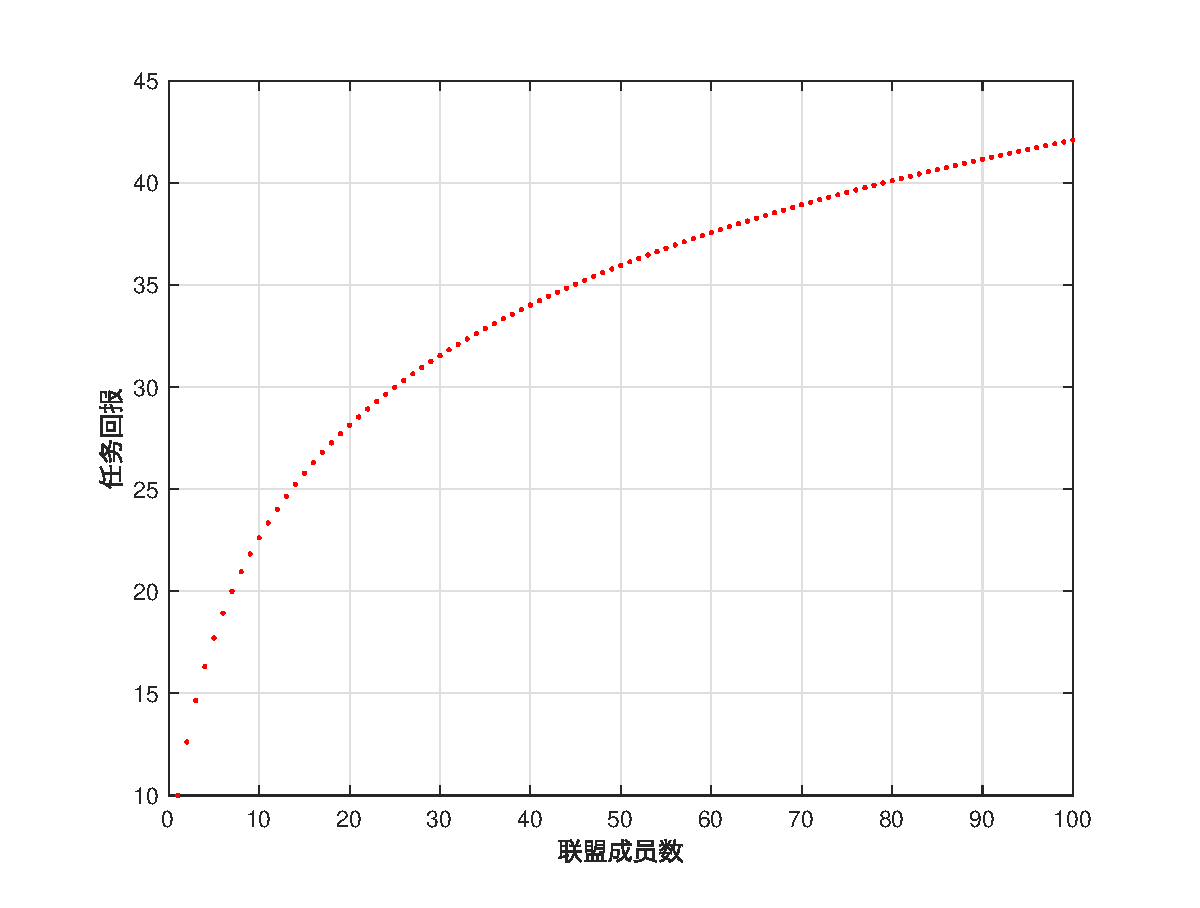
\includegraphics[scale=0.3]{taskreward.eps}}
  \hspace{2cm}
  \bisubcaptionbox{智能体回报函数}%
                  {Agent Reward Function}%
                  {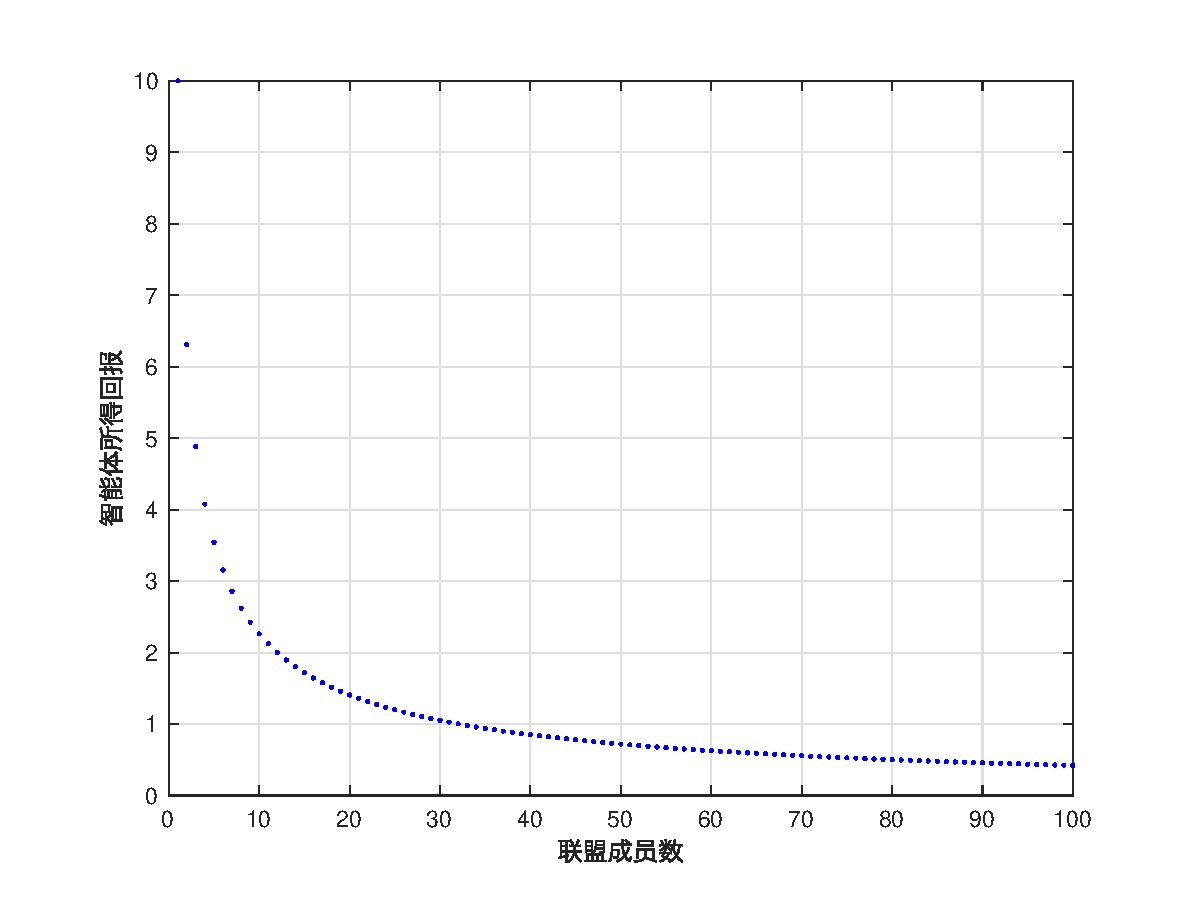
\includegraphics[scale=0.3]{agentreward.eps}}
  \bicaption{HCG模型的回报函数}
            {Reward Function of HCG Model}
  \label{hcg:fig:rewardfunc}
\end{figure}

与第\ref{chap:pg}章中遇到的约束条件处理问题类似,在本章使用HCG模型的场景中,需要限定得到的联盟划分满足约束条件式(\ref{model:eq:bmax})。由于本节定义的智能体效用函数与联盟成员数有关,而约束条件也是对于执行同一任务的智能体个数的限定,因此可以直接对智能体效用函数进行进一步改进,使得智能体在加入一个联盟时,会考虑到加入该联盟后该联盟成员数是否仍满足约束条件。如果加入该联盟后约束条件不再满足,则智能体不会选择加入该联盟。具体来说,引入改进智能体效用函数$\widetilde U_i(\mathcal{T}_j,|S_j|)$为

\begin{equation}
\label{hcg:eq:modifiedAgentU}
	\widetilde U_i(\mathcal{T}_j,|S_j|) = 
	\begin{cases}
		U_i(\mathcal{T}_j,|S_j|),\ & \text{if $|S_j|\leq b_{\text{max}}^{(j)}$,}\\
		0,\ & \text{otherwise}
	\end{cases}
\end{equation}

当智能体即将选择加入的联盟已经达到约束边界时,若智能体加入,则得到的效用将会是0,因此智能体最终不会选择再加入该联盟,从而保证了求解的可行性。

%---------------------------
%---------------------------
\section{基于享乐联盟博弈模型的决策算法}
\label{hcg:decision}

\subsection{SAP算法}
在HCG模型下的智能体决策算法仍可使用第\ref{chap:pg}章\ref{pg:pgta:protocal}节中使用的几种决策算法,本节选择使用SAP算法,下面算法\ref{hcg:algo:HCGSAP}将直接给出使用SAP的HCG决策算法流程。

\begin{algorithm}[htb]
	\caption{使用SAP的HCG决策算法流程}
	\label{hcg:algo:HCGSAP}
	\small
	\SetAlgoLined
	\KwIn{$\mathcal{M},\mathcal{T},\mathcal{A},r$}
	\KwOut{均衡解$a^*$}
	\tcp{初始化参数}
	$k \gets 1$\;
	随机生成任务分配初始解$a(0)$\;
	\tcp{计算初始每个任务联盟的成员数}
	$\text{CoWorkerNums}_j(0) \gets \sum_{\mathcal{M}_i \in \mathcal{M}} I\{a_i(0)=\mathcal{T}_j\}$\;
	\While{true}{
		随机选择一个智能体$\mathcal{M}_i$\;
		$n_i=|\mathcal{A}_i|$\;
		\For{$j=1:n_t$}{
			根据式(\ref{hcg:eq:agentU_reward})计算$U_i(\mathcal{T}_j,|S_j|+1)$\;
		}
		根据式(\ref{pg:eq:sappdf})计算$p_i(k)$\;
		根据$p_i(k)$随机选择任务$\mathcal{T}_l$\;
		\tcp{更新联盟划分和联盟成员数}
		$a_i(k) \gets  \mathcal{T}_l$\;
		$\text{CoWorkerNums}_{a_i(k-1)}(k) \gets \text{CoWorkerNums}_{a_i(k-1)}(k) - 1$\;
		$\text{CoWorkerNums}_{a_i(k)}(k) \gets \text{CoWorkerNums}_{a_i(k)}(k) + 1$\;
		$k\gets k+1$\;
	}
\end{algorithm}

%----------------------------
\subsection{分布式互斥算法}

本节将提出HCG模型下的另一种决策算法,称为互斥算法(Mutual Exclusion Algorithm, MEA)。MEA在每次迭代中,所有智能体都会做出自己的决策,但智能体在交互中会只保留一个智能体的决策结果。算法\ref{hcg:algo:decsion}和算法\ref{hcg:algo:dmea}给出了使用MEA的分布式决策算法,其中算法\ref{hcg:algo:decsion}是智能体$\mathcal{M}_i$在每次迭代的决策过程,算法\ref{hcg:algo:dmea}是MEA的实现。

\begin{algorithm}[htb]
	\caption{智能体$\mathcal{M}_i$的决策算法流程}
	\label{hcg:algo:decsion}
	\small
	\SetAlgoLined
	\KwIn{$\mathcal{M},\mathcal{T},\mathcal{A},r$}
	\KwOut{联盟划分$\Pi$}
	\tcp{初始化参数}
	$\text{satisfied} \gets false$\;
	$\text{evolved}^i\gets 0$;\tcp{智能体更新决策次数}
	$\text{stamp}^i \gets 0$;\tcp{时间戳}
	$\Pi^i \gets \{S_0=\mathcal{M},S_j=\emptyset, \forall \mathcal{T}_j \in \mathcal{T} \}$\;
	\While{true}{
		\tcp{每次迭代智能体做出新决策}
		\If{$\text{satisfied}=false$}{
			$(\mathcal{T}_{j^*},|S_{j^*}|) \gets \arg \max_{S_j \in \Pi^i} U_i(\mathcal{T}_j,|S_j \cup \{\mathcal{M}_i\}|)$\;
			\If{$(\mathcal{T}_{j^*},|S_{j^*}|)\succ_i (\mathcal{T}_{\Pi^i(i)},|S_{\Pi^i(i)}|)$}{
				智能体$\mathcal{M}_i$加入$S_{j^*}$,更新划分$\Pi^i$\;
				$\text{evolved}^i \gets \text{evolved}^i+1$\;
				$\text{stamp}^i \gets \mathrm{rand}[0,1]$\;
			}
		$\text{satisfied}\gets true$\;
		}
	智能体$\mathcal{M}_i$向邻居发送信息$I^i=\{\text{evolved}^i,\text{stamp}^i,\Pi^i\}$,并从其邻居节点获取信息$I^k,\forall \mathcal{M}_k \in \mathcal{N}_i$\;
	构造信息集$\mathcal{I}^i=\{I^i\}\cup\{I^k,\forall \mathcal{M}_k \in \mathcal{N}_i\}$\;
	\tcp{运行互斥算法}
	$\{\text{evolved}^i,\text{stamp}^i,\Pi^i\}, \text{satisfied} \gets \text{DMEA}(\mathcal{T}^i)$\;
	}
	
\end{algorithm}

\begin{algorithm}[htb]
	\caption{分布式互斥算法(DMEA)}
	\label{hcg:algo:dmea}
	\small
	\SetAlgoLined
	\KwIn{$\mathcal{I}^i$}
	\KwOut{$\{\text{evolved}^i,\text{stamp}^i,\Pi^i\},\text{satisfied}$}
	\tcp{初始化参数}
	$\text{satisfied} \gets true$\;
	\For{$M_k \in \mathcal{M}^i$}{
		\If{$(\text{evolved}^k>\text{evolved}^i)\ \text{or}\ (\text{evolved}^k=\text{evolved}^i\ \text{and}\ \text{stamp}^k > \text{stamp}^i)$}{
			$\text{evolved}^i \gets \text{evolved}^k$\;
			$\text{stamp}^i \gets \text{stamp}^k$\;
			$\Pi^i \gets \Pi^k$\;
			$\text{satisfied} \gets false$\;
		}
	}
\end{algorithm}

每个智能体在决策过程中都有自己的划分方式$\Pi^i$;变量satisfied是一个布尔变量,用于表示智能体是否对当前划分$\Pi^i$满意,即不会离开当前联盟;$r^i \in \mathbb{N}$是表示智能体做出了新决策,改变了联盟划分的次数;$s^i \in [0,1]$是一个服从0到1之间平均分布的随机变量,它会在划分$\Pi$每次更新时被生成,作用是作为一种时间戳,用于在后续交互时提供一致的依据。智能体在每次迭代中的决策过程是这样的:首先根据当前已知的划分$\Pi^i$,检查在该划分下,假设其他智能体不改变联盟,找出自己加入哪个联盟会得到最高效用(算法\ref{hcg:algo:decsion}第7行)。如果加入该联盟所得效用比自己当前联盟可得到的效用更高,则智能体会选择加入新联盟,同时增价更新次数$r^i$,并随机生成一个时间戳$s^i$(算法\ref{hcg:algo:decsion}第8-11行)。

由于每个智能体存储的都是自己的划分方式,因此在进行交互协商时,为了达成一致,只能有一种划分方式被广泛接受,称这个划分方式为有效划分。算法\ref{hcg:algo:dmea})介绍的MEA使得智能体能够在局部通信的情况下获得有效划分。智能体交互时传递的信息集为$I^i=\{\text{evolved}^i,\text{stamp}^i,\Pi^i\}$,包括自己的划分方式,划分更新次数和更新时间戳。在交互时,更新次数更多的划分方式被认为更加有效,如果更新次数一样,则选择时间戳更大的划分方式(算法\ref{hcg:algo:dmea}第3行)。在确定更有效的划分方式后,智能体将自己的划分方式、更新次数和时间戳统一为有效划分的对应值,同时将自己的满意值置为false使得智能体会在下次迭代做出新的决策(算法\ref{hcg:algo:dmea}第4-7行)。


%------------------------------------------
\subsection{模型与算法性能分析}
\label{hcg:performance}

%------------------------------------------
\subsubsection{收敛性分析}
\label{perform:convergence}

对于HCG模型下的任务分配算法收敛性,有如下定理。

\begin{theorem}[收敛性]
\label{hcg:tm:convergence}
	若HCG模型$\mathcal{G}$下的智能体都具有SIC性质,则$\mathcal{G}$收敛到一个纳什均衡划分的迭代次数至多为$|\mathcal{M}|\cdot(|\mathcal{M}|+1)/2$。
	\begin{proof}
		证明可以从只包含一个智能体的模型开始,逐一在模型中增加智能体并且找到新模型的纳什均衡划分。由定理1的证明过程可知,当一个新的智能体加入一个已得到纳什均衡划分的模型时,至多需要原有智能体个数加一次策略改变,新的模型就可以获得新的纳什均衡划分。因此可得,对于含有$|\mathcal{M}|$个智能体的模型,要获得其纳什均衡划分,至多需要的迭代次数为
		\begin{equation}
		\label{hcg:eq:maxIter}
			\sum_{k=1}^{|\mathcal{M}|} k = \frac{|\mathcal{A}|\cdot(|\mathcal{A}|+1)}{2}
		\end{equation}
		
	\end{proof}
\end{theorem}

而实际在使用\ref{hcg:decision}小节中的决策算法的场景下,不必像定理\ref{hcg:tm:convergence}的证明中在等到所有智能体达到纳什均衡后再加入新的智能体,因此实际迭代次数会小于定理中给出的上界。


%
\subsubsection{复杂度分析}
\label{perform:complexity}

假设算法\ref{hcg:algo:decsion}中在每次迭代过程中智能体进行的主要流程,即第6-17行,为一个迭代步。由于智能体之间的通信架构特点,可能存在着某些智能体的迭代步只是执行了发送信息的工作,并没有改变自身的信息(如$\Pi^i,\text{evolved}^i,\text{stamp}^i$),将这种迭代称为伪迭代过程,与其他改变了信息的正常迭代区分开来。

注意到在一次正常迭代发生前,伪迭代至多只会发生$d_G$次,$d_G$为通信网络的直径。因此根据定理\ref{hcg:tm:convergence}可知,模型收敛到纳什均衡所需的迭代步数为$O(d_G n_m^2)$。特别地,如果通信网络是全连通,则$d_G=1$,迭代步数变为$O(n_m^2)$。

接着考虑每次迭代过程中的计算复杂度。每个智能体在一次迭代中需要比较包括$\mathcal{T}_0$在内的$n_t+1$个任务联盟,因此计算复杂度为$O(n_t)$,结合前文所述的迭代步数复杂度,可知算法的总复杂度为$O(d_G n_t n_m^2)$。但注意到定理\ref{hcg:tm:convergence}的结果是保守的,因此实际复杂度会比上述结果更小。



%-----------------------------------------
\subsubsection{优化性能分析}
\label{perform:optimality}

关于HCG模型下得到的纳什均衡最优值和全局最优相比较的结果,可类比于命题\ref{pg:pro:PoA}的证明得到HCG模型$\mathcal{G}_{\text{HCG}}$的PoA指标上界为
\begin{equation}
\label{hcg:eq:PoA}
	\mathrm{PoA}(\mathcal{G}_{\text{HCG}}) \leq 1+\eta_{\text{HCG}},
\end{equation}
其中
\begin{equation}
\label{hcg:eq:eta}
	\eta_{\text{HCG}} = \sum_{S_j \in \Pi} \max_{\mathcal{M}_i \in \mathcal{M},p\leq |\mathcal{M}|} \big\{p \big[U_i(\mathcal{T}_j,p) - U_i(\mathcal{T}_j,|S_j \cup\{\mathcal{M}_i\}| \big] \big\}
\end{equation}

下面将针对前文所定义的智能体效用函数这一特殊情况,推导出关于PoA上界的更具体的结论。此处暂时性地引入任务效用函数概念$U_{\mathcal{T}_j}(\mathcal{T}_j,p)$,定义任务效用函数为执行该任务的所有智能体效用之和,即

\begin{equation}
\label{hcg:eq:taskU}
	U_{\mathcal{T}}(\mathcal{T}_j,p) = \sum_{\mathcal{M}_i \in S_j} U_i(\mathcal{T}_j,|S_j|).
\end{equation}

结合全局效用函数的定义式(\ref{hcg:eq:gloablU})有

\begin{equation}
\label{hcg:eq:taskU_to_globalU}
	U_g(a) = \sum_{\mathcal{M}_j \in \mathcal{M}} U_i(a_i,p_i) = \sum_{\mathcal{T} \in \mathcal{T}} U_{\mathcal{T}_j}(\mathcal{T}_j,p)
\end{equation}

若使用式(\ref{hcg:eq:agentU_reward})定义的智能体效用函数,使得任务效用函数$r(\mathcal{T}_j,p)$满足关于智能体数量$p$单调递增的性质,则可以进一步限定PoA的上界,实际上可得到如下命题。

\begin{proposition}
	设HCG模型$\mathcal{G}_{\text{HCG}}$中智能体效用函数$U_i(\mathcal{T}_j,|S_j|)$定义为式(\ref{hcg:eq:agentU_reward}),且$\varepsilon_j=\varepsilon>1$,则$\mathrm{PoA}(\mathcal{G}_{\text{HCG}})$满足
	\begin{equation}
	\label{hcg:eq:PoAforU}
		\mathrm{PoA}(\mathcal{G}_{\text{HCG}}) \leq 1 + \eta_{\text{HCG}}'
	\end{equation}
	其中
	\begin{equation}
	\label{hcg:pro:eq:etapie}
		\eta' = \log_{\varepsilon}(n_m+\varepsilon) -1
	\end{equation}
	
	\begin{proof}
		首先引入一个符号$\oplus$。给定两个划分$\Pi^A = \{S_0^A,\dots,S_{n_t}^A\}$和$\Pi^B = \{S_0^B,\dots,S_{n_t}^B\}$,$\Pi^A \neq \Pi^B$,
		\begin{equation}
		\label{hcg:pro:eq:oplus}
			\Pi^A \oplus \Pi^B := \{S_0^A \cup S_0^B, S_1^A \cup S_1^B, \dots, S_{n_t}^A \cup S_{n_t}^B \},
		\end{equation}
		由于$\cup_{j=0}^{n_t} S_j^A = \cup_{j=0}^{n_t} S_j^B = \mathcal{M}$,因此可能存在一个智能体$\mathcal{M}_i$在$\Pi^A \oplus \Pi^B$的两个不同联盟中出现了两次,但在此处我们分析时将这种出现了两次的智能体看做是两个不同的智能体。
		
		由式(\ref{hcg:eq:agentU_reward})定义的智能体效用函数,使得任务效用函数$r(\mathcal{T}_j,p)$满足关于智能体数量$p$单调递增的性质,另外全局效用函数为任务效用函数之和,因此对全局效用函数有
		\begin{equation}
		\label{hcg:pro:eq:oplus_inequility}
			U_g(\Pi^A) \leq U_g(\Pi^A \oplus \Pi^B).
		\end{equation}
		
		将全局最优划分$\Pi^{\text{opt}}$和纳什均衡划分$\Pi^*$分别取代上式中的$\Pi^A$和$\Pi^B$,则不等式左侧为即为全局最优效用$U_g(\Pi^{\text{opt}})$,不等式右侧可写为
		
		\begin{equation}
		\label{hcg:pro:eq:inequlity}
			U_g(\Pi^{\text{opt}} \oplus \Pi^*) = \sum_{\mathcal{T}_j \in \mathcal{T}_{\Pi^*}} U_{\mathcal{T}} \Big(\mathcal{T}_j, |S_j^{\text{opt}} \cup S_j^*|\Big) + \sum_{\mathcal{T}_k \in \mathcal{T}^-} U_i\Big(\mathcal{T}_k, |S_k^{\text{opt}} \cup S_k^*|\Big),
		\end{equation}
		其中$\mathcal{T}^-$为在$\Pi^*$中满足$S_j^* = \emptyset, S_j^{\text{opt}} \neq \emptyset$的任务$\mathcal{T}_j$集合。但在实际场景中认为除$\mathcal{T}_0$以外各任务均有智能体去执行,因此实际上$\mathcal{T}^- = \emptyset$,所以式(\ref{hcg:pro:eq:inequlity})实际上等于
		\begin{align}
			U_g(\Pi^{\text{opt}} \oplus \Pi^*) &= \sum_{\mathcal{T}_j \in \mathcal{T}_{\Pi^*}} U_{\mathcal{T}} \Big(\mathcal{T}_j, |S_j^{\text{opt}} \cup S_j^*|\Big)\notag\\
			&= \sum_{j=1}^{n_t} U_{\mathcal{T}} \Big(\mathcal{T}_j, |S_j^{\text{opt}} \cup S_j^*|\Big).
		\end{align}
			
		 代入式(\ref{hcg:eq:task_reward}),其中总代价函数$C=2\sum_{i=1}^{n_m} \sum_{j=1}^{n_t} c_i(\mathcal{T}_j)$是一常数,因此推导时暂时忽略,不会影响最终结果,将上式等号右侧化为
		
		\begin{align}
			&\ \sum_{j=1}^{n_t} U_{\mathcal{T}}\Big(\mathcal{T}_j,|S_{\Pi^*(i)}^j \cup S_j^*|\Big)\notag\\
			&= \sum_{j=1}^{n_t} r_j^0 \log_{\varepsilon_j} \big(|S_j^{\text{opt}} \cup S_j^*| + \varepsilon_j - 1\big)\notag\\
			&\leq \sum_{j=1}^{n_t} r_j^0 \log_{\varepsilon_j} \big(|S_j^{\text{opt}}| + |S_j^*| + \varepsilon_j - 1\big)\notag\\
			\label{hcg:pro:eq:expand}&= \sum_{j=1}^{n_t} r_j^0 \Big[ \frac{\log_{\varepsilon_j} \big(|S_j^{\text{opt}}| + |S_j^*| + \varepsilon_j - 1\big)}{\log_{\varepsilon_j}\big(|S_j^*|+ \varepsilon_j - 1\big)} \cdot \log_{\varepsilon_j}\big(|S_j^*|+ \varepsilon_j - 1\big)\Big].
		\end{align}
		
		若令$x=|S_j^*|,y=|S_j^{\text{opt}}|$,并代入$\varepsilon_j = \varepsilon>1$,由
		
		\begin{equation}
			\frac{\log_{\varepsilon}(x+y+\varepsilon-1)}{\log_{\varepsilon}(x+\varepsilon-1)} \leq \frac{\log_{\varepsilon}(n_m+\varepsilon)}{\log_{\varepsilon}(\varepsilon)} = \log_{\varepsilon}(n_m+\varepsilon),\ 1\leq x \leq x_m,\ 1 \leq y \leq n_m,
		\end{equation}
		
		因此
		
		\begin{align}
			\label{hcg:pro:eq:oplus_leq_nash}
			U_g(\Pi^{\text{opt}} \oplus \Pi^*) &\leq \sum_{j=1}^{n_t} r_j^0 \Big[\log_{\varepsilon}(n_m+\varepsilon) \cdot \log_{\varepsilon}\big(|S_j^*|+ \varepsilon - 1\big) \Big]\notag\\
			&= \log_{\varepsilon}(n_m+\varepsilon) \sum_{j=1}^{n_t} r_j^0 \Big[\log_{\varepsilon}\big(|S_j^*|+ \varepsilon - 1\big) \Big]\notag\\
			&= \log_{\varepsilon}(n_m+\varepsilon) U_g(\Pi^*).
		\end{align}
		
		而由式(\ref{hcg:pro:eq:oplus_inequility})可得
		\begin{equation}
		\label{hcg:pro:eq:opt_leq_oplus}
			U_g(\Pi^{\text{opt}}) \leq U_g(\Pi^{\text{opt}} \oplus \Pi^*).
		\end{equation}
		
		结合式(\ref{hcg:pro:eq:oplus_leq_nash})和式(\ref{hcg:pro:eq:opt_leq_oplus})即可得
		\begin{align}
		\label{hcg:pro:eq:PoA_max}
			U_g(\Pi^{\text{opt}}) &\leq \log_{\varepsilon}(n_m+\varepsilon) U_g(\Pi^*)\\
			\mathrm{PoA}(\mathcal{G}_{\text{HCG}}) &\leq 1+ \big[\log_{\varepsilon}(n_m+\varepsilon) -1\big]\notag\\
			&\triangleq 1+\eta'.
		\end{align}
		
				
		\end{proof}
\end{proposition}


\section{仿真分析与对比}
\label{hg:sec:simulation}

\subsection{算法性能对比}
\label{simu:sub:conpare}

\section{本章小结}
\label{hg:sec:conclusion}





% !TEX root = ../main.tex

\chapter{基于随机博弈模型的分布式动态任务分配框架}
\label{chap:stochastic}

\section{引言}
\label{sg:intro}

第\ref{chap:pg}章和第\ref{chap:hedonic}章是针对静态场景下的任务分配问题,但在解决第\ref{chap:model}章中提出的动态场景下的任务分配问题时,会面临两大问题:一是环境动态变化难以预测,如出现导弹通信网络变化,或目标数量可能出现变化等情况,使得求解模型中的重要变量,如任务效用函数发生变化,原纳什均衡被破坏;二是前两章提出的利用博弈理论提出的决策算法,由仿真结果可知最终收敛结果与收敛速度具有一定的波动性,实际上与算法开始迭代时的初始解有关。

为了解决以上问题,本章利用随机博弈模型建立了分布式动态任务分配框架,并根据实际场景中可能发生的事件,设计了任务重分配触发机制,在此基础上结合前两章的模型与算法,实现动态环境下的任务分配,并通过仿真结果验证了该框架具有较好动态自适应性。

\section{随机博弈模型}
\label{sg:stochastic_game}

随机博弈模型一般是有多个参与者参与的具有状态概率转移的动态博弈过程。下面的定义给出了随机博弈的概念。

\begin{definition}[随机博弈]
	随机博弈可用一组元组表示$\mathcal{G}=<N,\Omega,\{S_i,U_i\}_{i\in N},q>$,其中$N=\{1,2\dots,n\}$表示博弈参与者集合;$\Omega$表示模型所有的可能状态集合;对于每个可能状态$\omega \in \Omega$,都有一个与之相关的阶段博弈$\gamma(\omega)$,该博弈具有策略空间$S^\omega$和效用空间$U^\omega(s)$;$q(\omega^{t+1}|\omega^t,s)$是状态转移概率,表示在$t$时刻模型状态$w^t$下,参与者选择策略$s$后,模型在$t+1$时刻转移到状态$w^{t+1}$的概率。
\end{definition}

随机博弈一般具有多个阶段,在每个博弈阶段,博弈模型会处在一个特定状态中,参与者根据当前状态和预期回报选择自己的最优策略,接着模型会依据状态转移概率转入下一状态,从而开始新一轮博弈。博弈参与者被认为掌握当前状态的信息,且它所能得到的回报仅仅取决于当前状态和它在该状态下采取的策略,而状态转移概率分布完全由当前状态和参与者的决策策略决定。



\section{面向动态任务分配问题的随机博弈框架设计}
\label{sg:framework}

将随机博弈模型应用于导弹任务分配问题,实际上是将某一时刻的任务分配看作是整个模型的状态之一,参与分配的导弹(智能体)即为博弈的参与者,在每个时刻做出的决策即为选择目标。在选择目标后,导弹和目标的飞行会使得环境发生改变,因此下一时刻的任务分配问题便会发生改变。具体而言,本章基于随机博弈模型建立的任务分配框架包含以下几个部分:

(1)状态集合,为每个时刻的任务集合$\mathcal{T}(t), \mathcal{T}(t) \subseteq \mathcal{T}$,$t$为当前时刻;

(2)智能体集合$N=\{1,2\dots,i,\dots,n_m\}$,表示博弈的参与者,每个智能体拥有自己的策略集$\mathcal{A}_i(t) = \{a_k\}$,即为智能体的可选任务集合,且智能体效用函数定义为$U_i(a_i,a_{-i})$;

(3)状态转移概率函数$q(w^{t+1}|w^t)$;

(4)全局效用函数$U_g(a)$。

其中(1)、(2)中的任务集合和智能体集合可直接使用前两章中的概念,使用每个时刻参与分配的导弹和目标集合即可。对于(2)中的智能体效用,本章仍使用第\ref{chap:pg}章中的WLU效用和第\ref{chap:hedonic}章中的效用函数。(3)中的状态转移概率函数取决于模型框架的设计,(4)中的全局效用函数仍沿用前几章的定义。结合第\ref{chap:model}章\ref{model:dynamic_model}小节建立的动态环境模型的特点及可能面临的问题,下面将详细针对模型框架进行阐述。


\subsection{时间窗口划分}
\label{game_stage:time_window}

动态模型下每个时刻环境的状态都与前一时刻不同,一方面不可能对每一时刻建立任务分配模型进行求解,另一方面求解任务分配也需要时间。因此本文将攻击过程划分为若干时间窗口$[t,t+w]$,每一时间窗口作为一个博弈阶段,在同一窗口内,假设导弹和目标态势关系变化不大,最优任务分配结果不会发生改变,因此可以在一个时间窗口内建立起任务分配模型并求解。

时间窗口长度$w$的选取是一个需要权衡的问题。一方面,由于在一个窗口期内,认为态势变化不大,因此如果时间窗口过长,导弹和目标的位置已发生较大变化,态势变化不大的前提假设不再成立,且一些突发事件可能会被忽略而不能及时响应;另一方面,如果时间窗口过短,一方面可能任务分配结果可能还未解出,另一方面鉴于导弹的运动特性,如果频繁重分配可能导致弹道过于弯曲而造成能量浪费。

根据以上分析,结合第\ref{chap:model}、\ref{chap:pg}、\ref{chap:hedonic}章里的相关模型和假设,可以给出时间窗口长度$w$应该满足的条件为

\begin{equation}
\label{sg:eq:window}
	w \geq t_{\text C} + t_{\text A},
\end{equation}
其中,$t_{\text C}$表示导弹之间进行通信并达成信息一致所需的时间,$t_{\text A}$表示导弹进行任务分配决策达到收敛所需的时间。式(\ref{sg:eq:window})的含义是窗口时间的长度不得少于导弹需要完成信息交互和任务分配求解两个过程的时间。

\subsection{博弈子模型建立}
\label{game_stage:submodel}

根据前一小节论述,在划分出一段时间窗口后,需要在每个时间窗口期内建立一个博弈子模型以求解任务分配问题,并且此时可视为静态分配问题求解。因此本小节建立的博弈子模型是基于前两章提出的势博弈分配模型和享乐联盟博弈分配模型。

具体而言,在一个新的博弈阶段开始时,各导弹会根据\ref{model:dynamic_model}小节介绍的模型,统计自己可跟踪的目标以及可通信的导弹,并建立起新的通信网络。根据这些信息,建立势博弈分配模型或享乐联盟博弈分配模型,此时在博弈模型中需要明确各导弹的可选目标集,除了限定为可跟踪到的目标集合$\mathcal{A}^{\text{Detect}}_i$的子集,导弹还需要找出自身可攻击到的目标集合$\mathcal{A}^{\text{Attack}}_i$。结合导弹具有最大过载的特点,本文选择的目标是否可行的判据是:判断导弹攻击该目标所需要的制导过载指令是否会超出导弹的最大过载。设导弹最大过载为$g_{\text{max}}$,导弹在当前状态下攻击该目标预计过载指令为$a_{\text{M}}$,若$a_{\text{M}}>g_{\text{max}}$,则该目标不再是可选目标,所以最终各导弹的可选目标集为$\mathcal{A}_i = \mathcal{A}^{\text{Detect}}_i \cap \mathcal{A}^{\text{Attack}}_i$
。最优分配的求解具体过程与原理前两章已详细阐述,此处不再赘述。

\subsection{博弈阶段切换}
\label{game_stage:stage_transform}

在不同博弈阶段切换的时间点,除了导弹和目标的状态信息、导弹的通信网络发生变化需要更新外,最重要的是任务分配解的传递与切换。根据前面章节的论述和仿真实验可知,在一个博弈阶段内建立的分配模型所得到的最优分配解效果,以及算法收敛速度均与初始解有关。因此在新的博弈阶段子模型建立后,需要决定新的模型下开始算法迭代的初始分配解。如果每次都采用随机生成的解,则每次算法收敛到对应的纳什均衡解会造成时间的浪费,且前文已提到,随机生成的解最终可能得到不同的均衡解,甚至效果较差的均衡解;另一方面,如果一直采用前一阶段的分配解作为新阶段的初始解,则由于原分配解已经是纳什均衡解,且分配模型中的约束条件的存在,可能会限制导弹选择其他目标,使得模型陷入局部最优。

为解决该问题,本文使用的方法是,将前一时刻的分配解与随机生成解以一定概率进行交叉变异,生成新的分配解作为新的博弈阶段的初始解。每个导弹以一定概率$p$选择原分配解$a_k$作为初始解,以$1-p$的概率从$k+1$时刻可选目标集中随机选择一个目标$a_{\text{rand}}^j$作为初始解,则生成$k+1$时刻博弈模型的初始解$a_{k+1}(0)=\{a_{k+1}^1(0),a_{k+1}^2(0),\dots,a_{k+1}^{n_m}(0)\}$

\begin{equation}
\label{sg:eq:crossfactor}
	a_{k+1}^j(0) = I\{e<p\}a_k^j + I\{e \geq p\}a_{\text{rand}}^j,\ e = \mathrm{rand}(0,1).
\end{equation}

此处不需要考虑新解的可行性,因为博弈分配算法会自行消解分配冲突,其中原理前面章节已经论述。

切换过程需要考虑的另一个问题是,在上一个博弈阶段得到的任务分配解,是否接受并传递给下一博弈阶段。由于考虑到频繁切换目标会对导弹带来能量的消耗甚至最终不能成功击中目标,因此本文采用的是带惰性的传递方法,当导弹集群获得$k$时刻的分配结果时,若与当前结果不一致,则会以$q$的概率采用新分配,而以$1-q$的概率拒绝新分配。为了保持分配解的可行性,新分配解的接受或拒绝对所有导弹保持一致,即在同一个连通分支内的所有导弹只要有一枚导弹接受或拒绝新方案,该分支内所有导弹均会作出同样的选择。




\section{重分配触发机制}
\label{sg:special_incidence}

虽然在上述随机博弈框架下,假设在一个博弈阶段内态势不会发生重大变化,但实际情况中,发生足以需要重新分配的场景和事件仍是存在的。针对这类突发状况,需要制定一套事件触发机制,明确事件触发信号和触发后重分配方法。

\subsection{通信网络非连通}
\label{special:disconnected_network}

在第\ref{chap:model}章建立的任务分配模型中,导弹存在着通信半径,因此导弹之间建立的通信网络可能存在着非连通的情况。在此情况下,导弹集群往往会形成两个或多个连通分支,无法相互之间共享信息。在此情况下两个不在同一通信分支的导弹可能会生成相互冲突的分配解而无法消除,为了解决这一问题,首先需要引入以下命题。

\begin{proposition}[可消解冲突]
	如果两枚导弹之间不存在通信,则它们在一个博弈阶段内可以消解冲突的条件是
	\begin{equation}
	\label{sg:eq:collision}
		R_{\text{comm}} \geq 2 V_{\text{max}} T_k \Delta t + R_{\text{col}},
	\end{equation}
	其中,$V_{\text{max}}$表示导弹的最大速度,$T_k$表示第$k$个博弈阶段的时间步数,$\Delta t$表示单位时间周期,$R_{\text{col}}$表示导弹碰撞半径。
\end{proposition}

\begin{figure}[!htp]
  \centering
  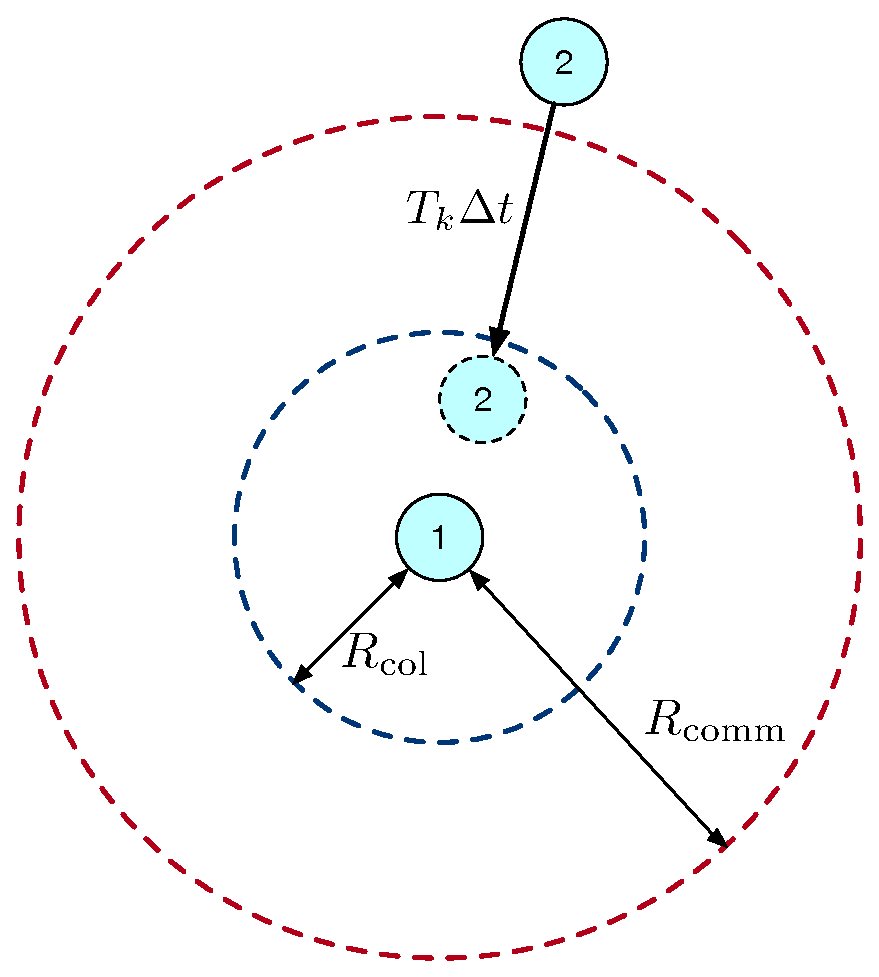
\includegraphics[height=6cm]{stochastic_game/undetectable_collision.eps}
  
  \bicaption[不可规避冲突]
  {不可规避冲突}
  {Illustration of an undetectable collision}
  \label{fig:undetectable_collision}
\end{figure}

在一个时间窗口的博弈阶段内,导弹不会改变分配目标,因此如果出现两个没有建立通信的导弹选择了同一目标产生冲突,则会由于制导律的作用相互靠近,若在时间窗口期内距离小于碰撞距离,则两枚导弹就会发生碰撞,这一过程如图\ref{fig:undetectable_collision}所示,在第k个博弈阶段刚开始时导弹2仍处于导弹1的通信半径(红色虚线圆)外,但在该阶段时间内,导弹2迅速进入了导弹1的最小碰撞半径范围(蓝色虚线圆),此时两导弹难以避免碰撞。

因此为了避免这种情况,对导弹通信半径施加上述条件,使得在同一窗口期内,导弹在碰撞前能够及时建立起通信关系。而新的通信关系一旦建立,会触发重分配条件,原先的分配解在新模型下不再是可行解,从而冲突会被消解,得到的新分配解会适用于新通信网络。这一过程示意图如图\ref{fig:collision_resolution}所示,导弹1和2(蓝色实线实心圆)同时选择了目标1(红色实心圆),但由于互相处于通信范围外(红色虚线圆),并未建立通信,因此冲突无法消解。但随着对目标的接近,两导弹之间的距离逐渐减小(蓝色实心虚线圆),且达到了建立通信的条件,此时触发重分配条件,立即结束当前博弈阶段,建立新的模型重新分配,因此导弹1会重新选择目标2,冲突由此消解。

\begin{figure}[!htp]
  \centering
  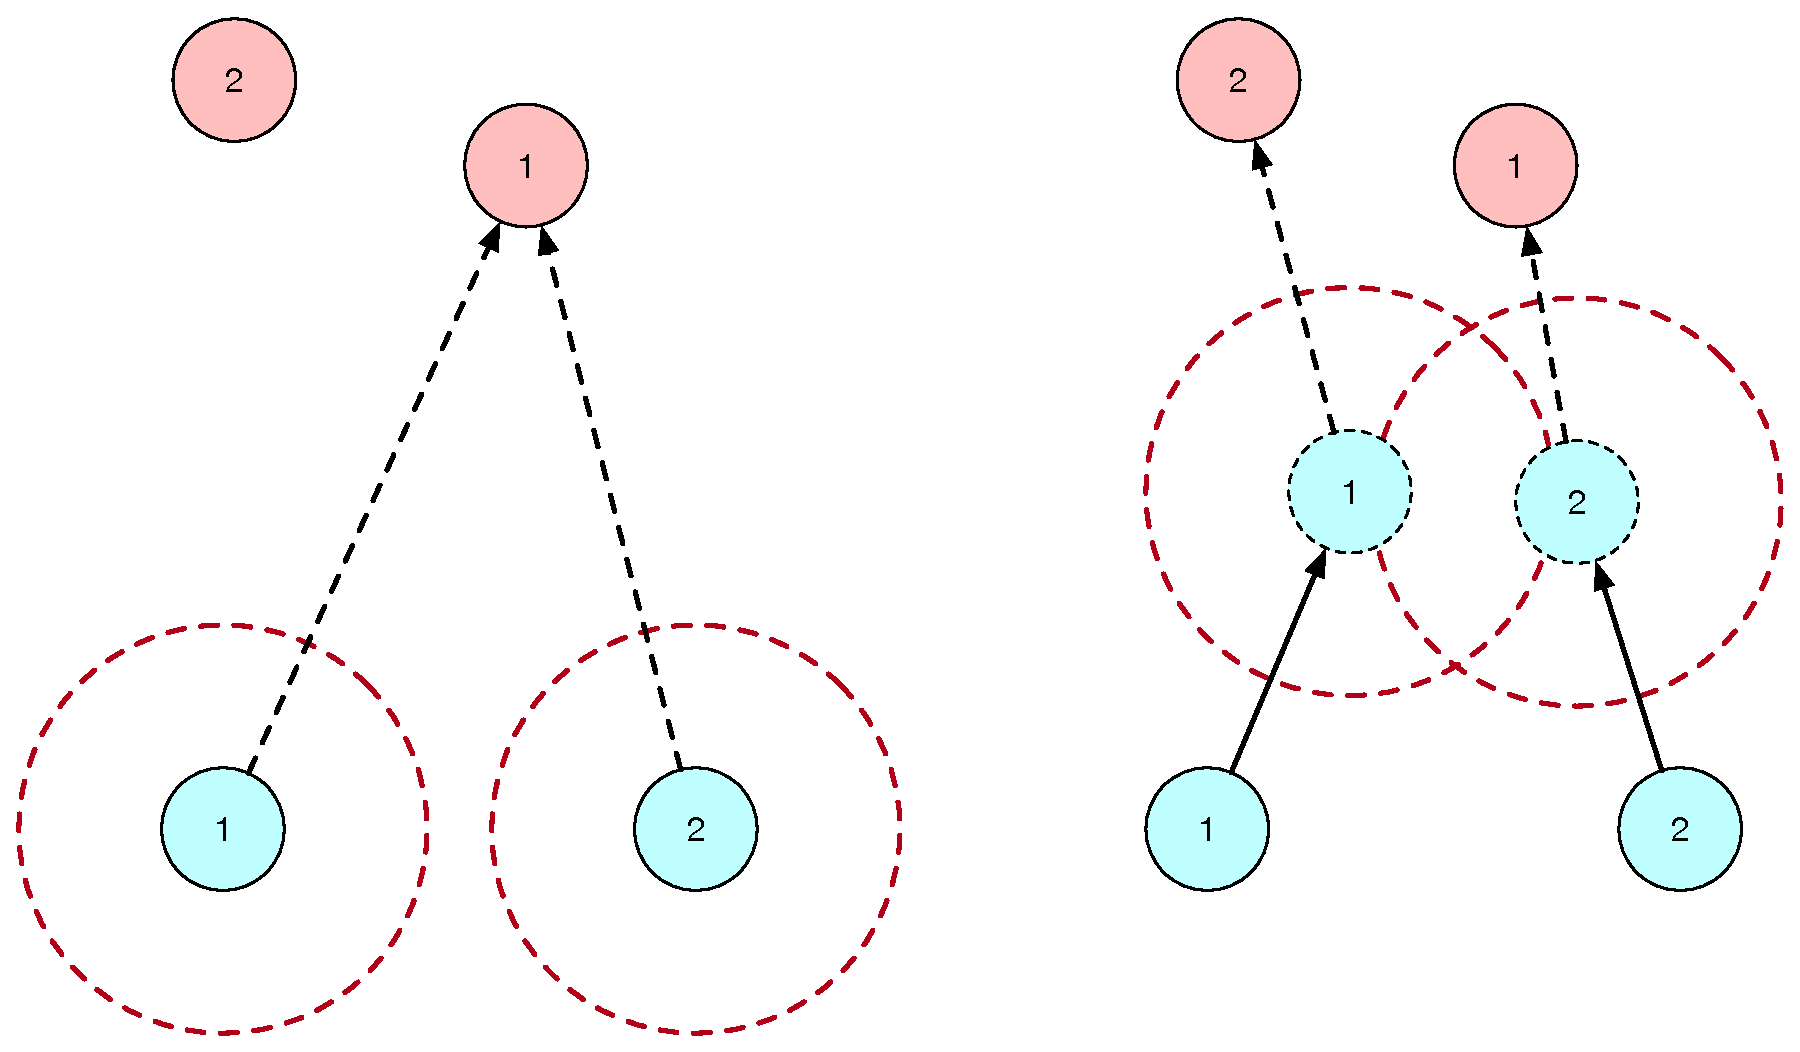
\includegraphics[height=6cm]{stochastic_game/collision_resolution}
  \bicaption[非连通场景下分配冲突消解示意图]
  {非连通场景下分配冲突消解示意图}
  {Resolution of an assignment conflict in the disconnected communication scenes}
  \label{fig:collision_resolution}
\end{figure}

\subsection{目标数量可变}
\label{special:target_num_change}

目标数量变化可分为目标数量增加和目标数量减少两种场景。目标增加的原因通常有两种:一是导弹发射前已知该目标,但导弹发射后该目标处于导弹探测区外,随着攻击过程的进行才进入导弹探测范围;二是导弹发射前该目标未出现或未被地面雷达或载机捕捉,在导弹飞行过程中被导弹自行捕获。本文不考虑原先被跟踪的目标逃出导弹探测范围的情况,因此目标减少的原因通常就是被导弹击中。

针对目标增加的第一种原因,由于导弹在发射前对于目标数量等信息已知,因此只需结束当前博弈阶段,触发重分配机制,建立新的博弈阶段并求解新的分配解即可,为了使得新探测到的目标进入分配解,在建立新博弈阶段时,首先发现该目标的导弹在确定初始解时不再使用式(\ref{sg:eq:crossfactor})所示的交叉算子,而是直接使用新目标作为初始解,由于在原分配中没有导弹选择新目标,因此在分配模型中新目标将会被保留,只能在导弹之间交换而不会被某个导弹单方面放弃。

针对目标增加的第二种原因,由于第\ref{chap:model}章模型建立中式(\ref{model:eq:bmax})的约束,因此在之前的讨论中导弹数量往往不会多于攻击所有已有目标所需的数量之和,而没有多余的导弹攻击新增的目标。假设新目标$\mathcal{T}_w$所需的导弹数量为$b_{\text{max}}^{(w)}$,在不考虑发射新的导弹的情况下,解决这一问题的方案是是改变现有模型,从原分配解中满足$b_{\text{max}}^{(j)}>1$的目标的攻击导弹中抽出$b_{\text{max}}^{(w)}$个导弹,用于攻击新目标\footnote{显然这种方案成立的条件是$n_m-n_t \geq b_{\text{max}}^{(w)}$,本文的讨论是基于满足该条件的场景下,对于不满足该条件的场景,本文不再讨论。}。

针对目标减少的场景,往往是由于导弹击中目标,因此也包含着导弹数量减少的场景。本章建立的模型中,导弹击中目标的判定条件是弹目距离小于指定阈值$R_{\text{min}}$代表目标进入导弹杀伤范围,或弹目相对接近速度$V_R>0$,代表弹目距离不再减小。此时击中目标数量若达到$b_{\text{max}}^{(j)}$,则目标被击落,攻击该目标的导弹也退出通信网络与分配模型。当一些导弹攻击完成后,其邻居节点可能失去连接通道,从而不再连通,此时将回到\ref{special:disconnected_network}小节中所论述的场景。

\section{系统设计与仿真验证}
\label{sg:system&simulation}

\subsection{动态任务分配系统设计}
\label{sg:dynamic_system}

结合\ref{sg:framework}节和\ref{sg:special_incidence}节的内容,图\ref{fig:framework}给出了动态环境下基于随机博弈模型的任务分配系统框图。

\begin{figure}[!htp]
  \centering
  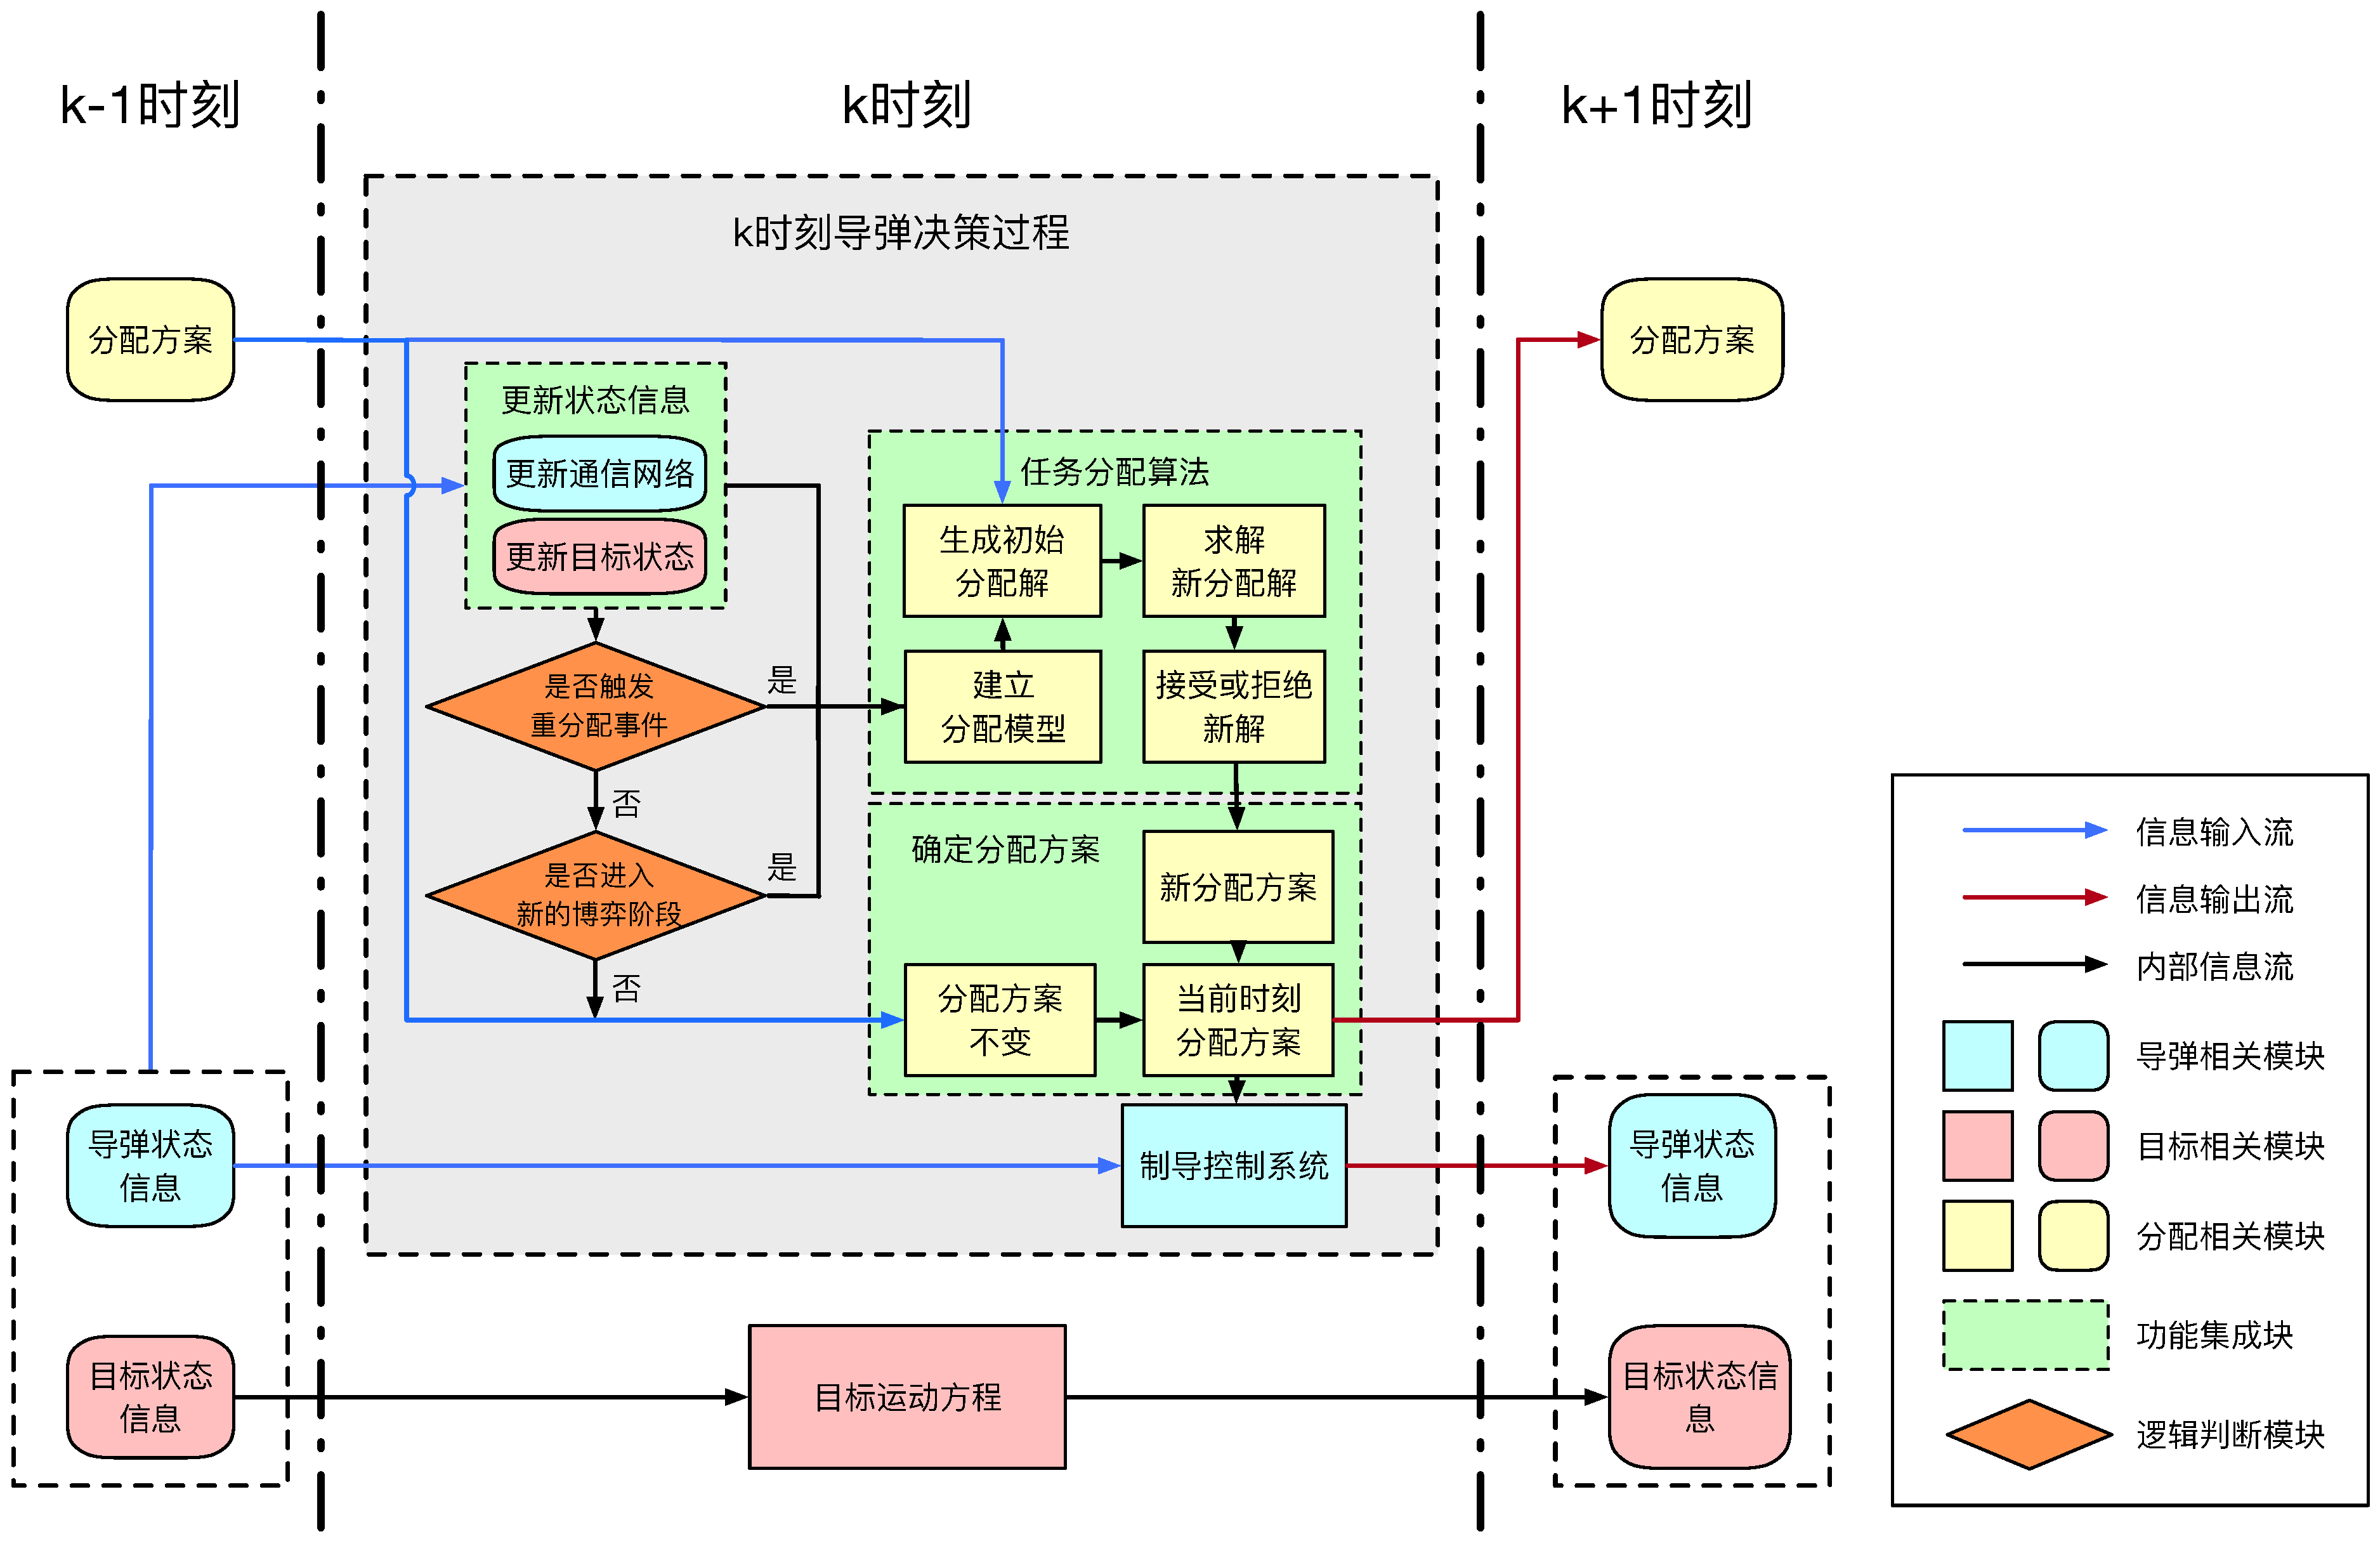
\includegraphics[height=10cm]{stochastic_game/framework}
  \bicaption[导弹任务分配系统框架示意图]
  {导弹任务分配系统框架示意图}
  {Illustration of framework of missiles task assignment system}
  \label{fig:framework}
\end{figure}

其中目标运动部分独立在外,不在控制范围内。导弹模块主要分为态势信息收集与更新、事件触发判断、任务分配和制导控制四个模块,各部分的主要功能为:

(1)态势信息收集与更新。在每个时刻导弹需要获知自身状态信息与可选目标信息,并寻找可建立通信关系的同伴,建立通信网络,共享目标信息。

(2)事件触发判断部分实现的功能是根据当前时刻收集到的导弹与目标状态信息,判断是否发生了需要立即重新分配的事件。根据上文的讨论,这些事件主要包括导弹通信网络的改变、新目标的出现和目标被导弹击中等场景。发现事件发生的导弹立即进入重分配过程,并将事件情况向可通信导弹发出,促使其他导弹也进入重分配过程。

(3)任务分配部分在两种场景下会被调用。一种是正常的博弈阶段结束,进入下一阶段时会获取新态势进行新的任务分配过程;另一种则是根据事件触发判断部分的结果,在正常阶段结束前提前进入重分配过程。该部分的主要流程是根据获取的态势建立分配模型,同时利用\ref{game_stage:stage_transform}小节中提出的初始解生成方法,生成代入求解模型的初始分配,在得到当前态势下收敛的分配解后,再以一定概率接受或拒绝该分配。

(4)制导控制部分负责根据导弹计算出的分配结果,计算制导制令,并控制导弹向指定的目标飞去。

在每个时间点,导弹不断重复以上四个步骤,直到该导弹击中目标即停止。当所有导弹均击中目标时,整个导弹集群任务分配系统停止运行。

\subsection{仿真实验}
\label{sg:simulation}

根据\ref{sg:dynamic_system}小节建立的动态任务分配系统,结合第\ref{chap:pg}章和第\ref{chap:hedonic}章建立的任务分配模型和算法,进行动态环境下的空空导弹任务分配仿真实验。实验中导弹和目标的初始位置、速度、角度等信息随机生成,目标以一定的加速度做机动运动,导弹在发射前可以根据地面雷达或载机收集到已探测到的目标状态信息,并生成初始分配解。在发射后,导弹进入”发射后不管“状态,即导弹与地面或空中平台不再建立通信,只依赖于互相之间的通信进行协同攻击。

\begin{figure}[!hbtp]
  \centering
  \bisubcaptionbox{平衡分配场景分配效果(5vs5)}%
                  {Performance of balance assignment scenario (5vs5)}%
                  {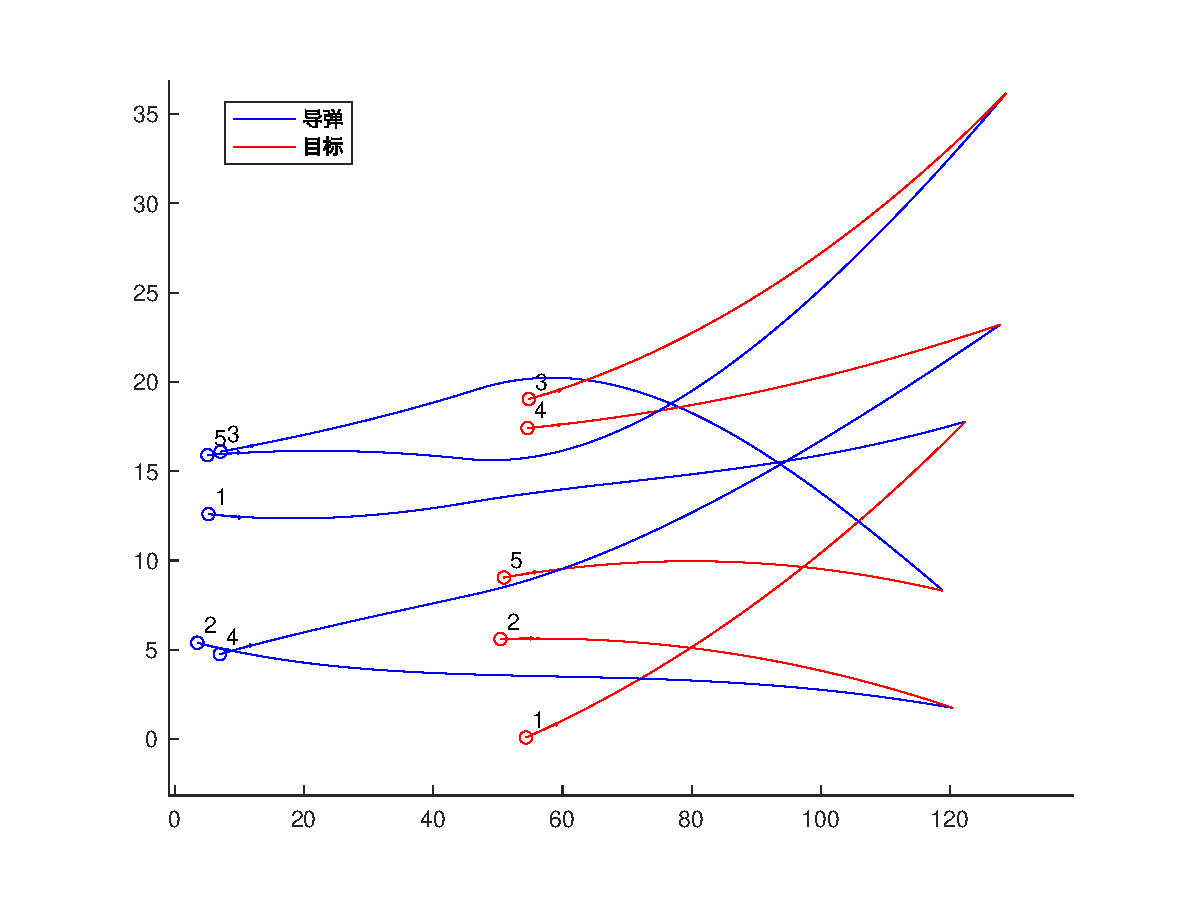
\includegraphics[height=8cm]{stochastic_game/SAP5vs5}}
  \bisubcaptionbox{非平衡场景分配效果(6vs4)}%
                  {Performance of unbalance assignment scenario (6vs4)}%
                  {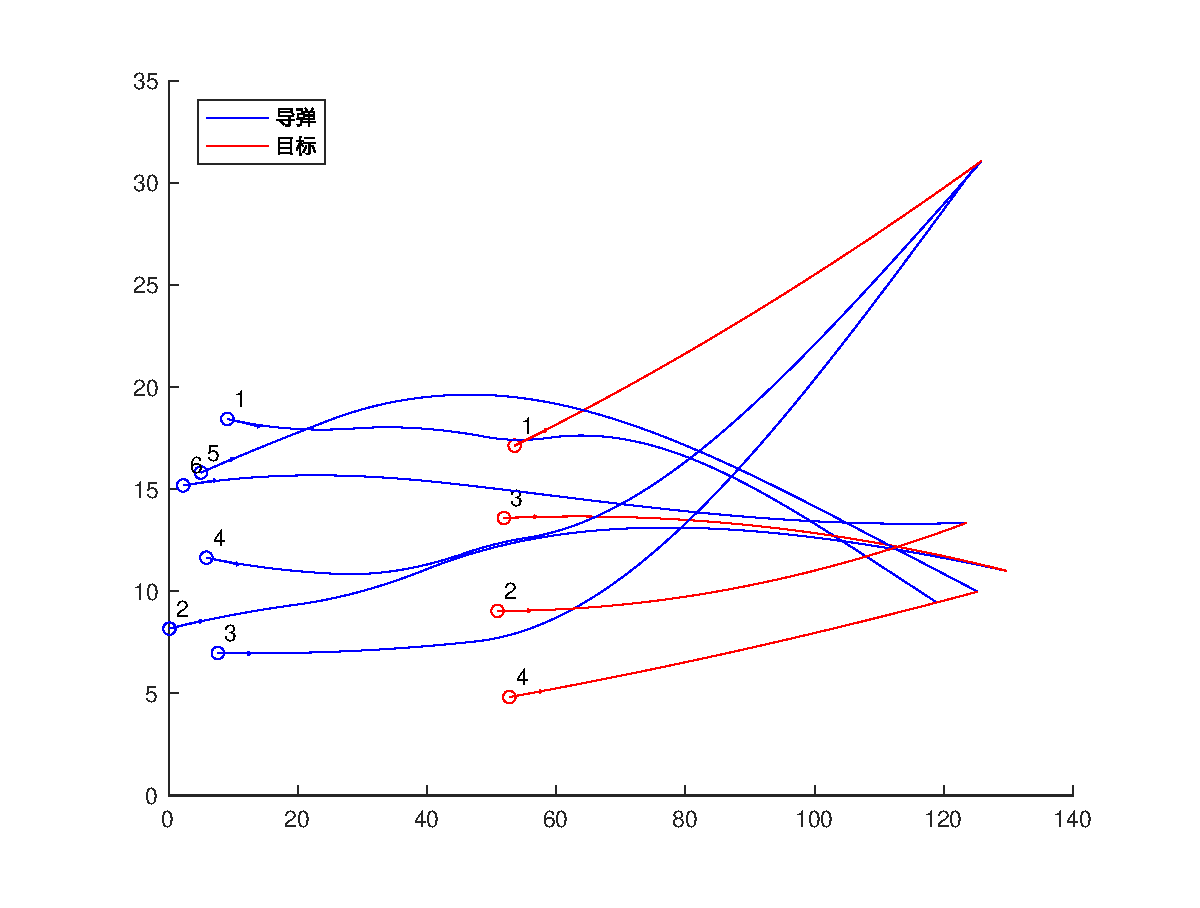
\includegraphics[height=8cm]{stochastic_game/SAP6vs4}}
  \bicaption{基于势博弈模型的动态任务分配效果}
            {Dynamic task assignment based on potential game model}
  \label{sg:fig:pg}
\end{figure}

\begin{figure}[!hbtp]
  \centering
  \bisubcaptionbox{平衡分配场景分配效果(5vs5)}%
                  {Performance of balance assignment scenario (5vs5)}%
                  {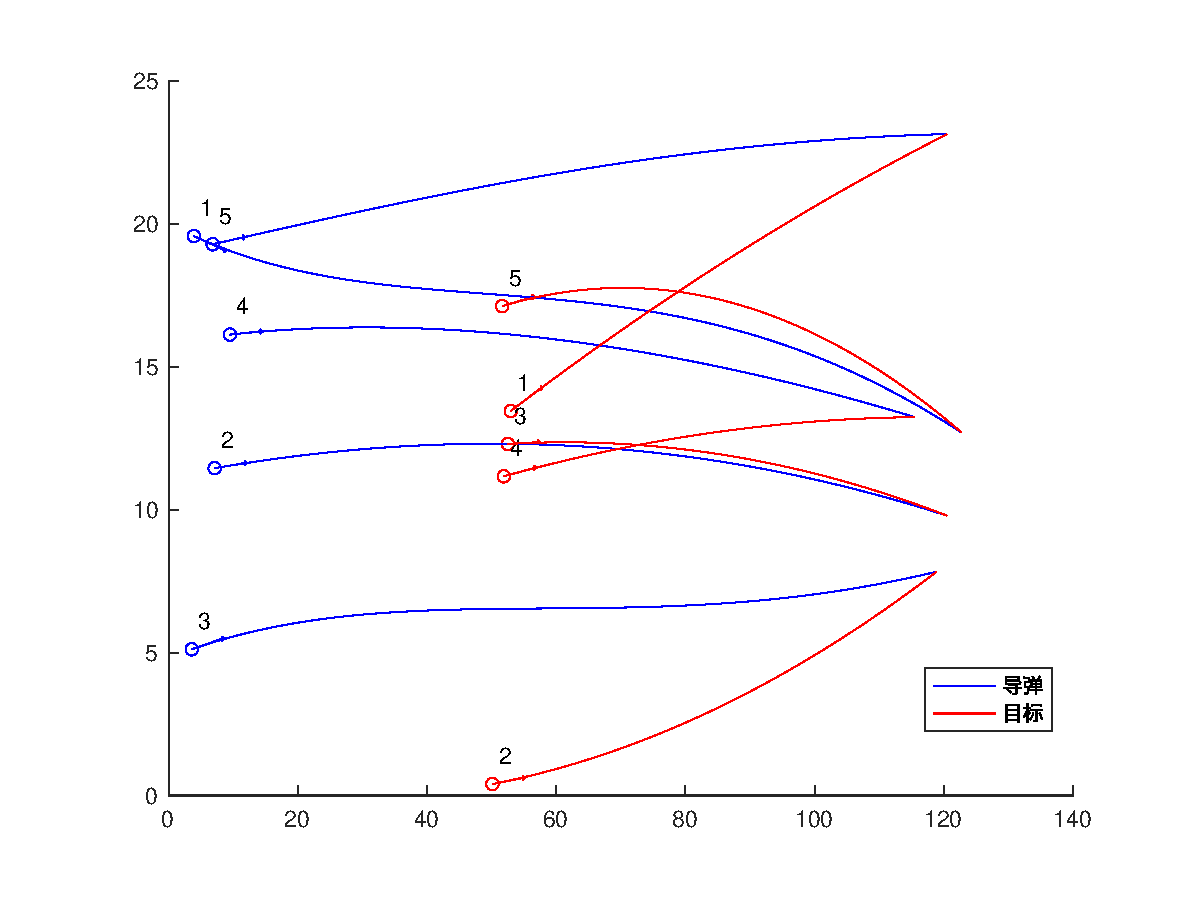
\includegraphics[height=8cm]{stochastic_game/HCG5vs5}}
  \bisubcaptionbox{非平衡场景分配效果(6vs4)}%
                  {Performance of unbalance assignment scenario (6vs4)}%
                  {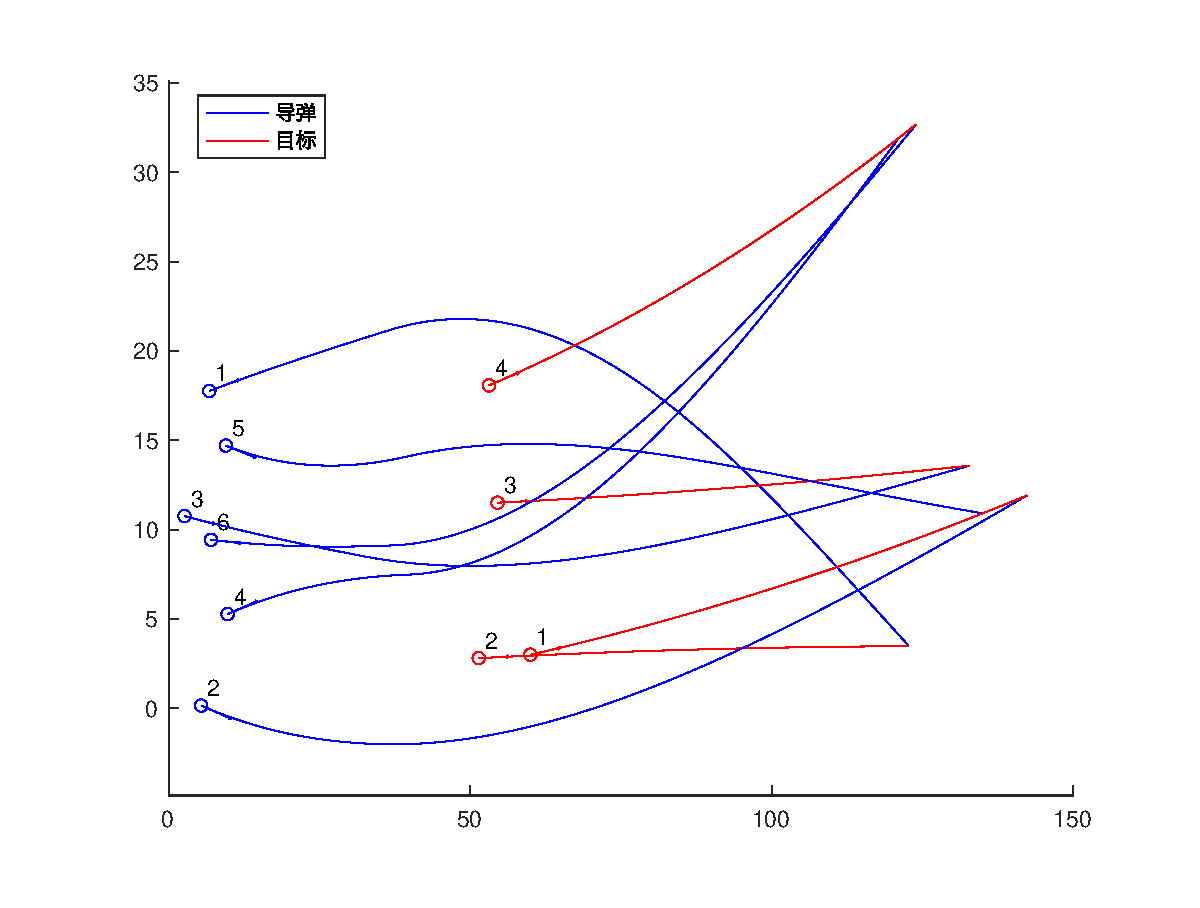
\includegraphics[height=8cm]{stochastic_game/HCG6vs4}}
  \bicaption{基于HCG模型的动态任务分配效果}
            {Dynamic task assignment based on HCG model}
  \label{sg:fig:hcg}
\end{figure}

图\ref{sg:fig:pg}和图\ref{sg:fig:hcg}分别展示的是使用势博弈模型和HCG模型的动态任务分配结果,图\ref{sg:fig:pg}(a)和图\ref{sg:fig:hcg}(a)展示的是平衡分配场景(5vs5)的分配效果,可以看出所有导弹都被分配到一个目标,且导弹的轨迹相对平滑,说明在此情况下导弹在攻击过程中更改目标的次数不多。而图\ref{sg:fig:pg}(b)和图\ref{sg:fig:hcg}(b)展示的是非平衡分配场景(6vs4)下的分配效果。由图中可以看出,相比平衡分配,在非平衡分配下导弹轨迹更加曲折,说明导弹在中途更换了目标,这表明在飞行过程中导弹态势的变化较大,且对于需要多个导弹攻击的目标,导弹之间相对位置的变化,以及目标的机动可能会导致导弹选择不同的队友进行协同攻击。此外,导弹轨迹在攻击后期往往是较为平滑的,这是因为当接近目标的时候,导弹对于各自目标的优势已经足够明显,而此时更换目标所需的时间和机动能量成本过大,因此此时导弹往往不会再更换分配方案。

以上仿真场景中,导弹与目标的状态都假定是事先已知,且导弹通信网络为全连通网络。为了验证本章提出的动态任务分配系统在非理想场景下的有效性,下面将针对\ref{sg:special_incidence}小节中讨论的两种重分配场景进行仿真验证。

(1)通信网络非连通

为了验证在通信网络非连通场景下的系统有效性,将仿真场景设置为导弹初始位置分为两个独立的集群,集群之间距离大于导弹的通信半径,因此两集群之间在初始时没有通信关系。在攻击过程中,两集群可以各自独立地对目标进行跟踪和分配。


图\ref{sg:fig:disconnected}表示的是10vs10场景下的导弹攻击过程。在初始时刻,1-5号导弹和6-10号导弹各形成一个集群,且彼此之间的距离超过了导弹的通信半径,因此这两集群之间不存在通信关系,并且部分目标超出了导弹探测范围。由图\ref{sg:fig:disconnected}(a)也可看出,在初始分配时,6-10号导弹中只有6号选择了9号目标,其余都选择了2号目标,因为其余目标都不在这个集群内导弹的探测范围内。值得注意的是,这里有部分目标,比如10号,处于所有导弹的探测范围外,因此在初始时刻没有导弹选择该目标。

当到了30s的时刻,如图\ref{sg:fig:disconnected}(b)所示,此时随着导弹之间距离的接近,两个集群间开始建立起通信,因此原本冲突的分配得到消解,比如原来集中选择2号目标的几枚导弹现在有了各自不同的目标。与此同时,由于导弹与目标的接近,原本不被任何导弹探测的目标现在也进入了导弹集群的探测范围,因而成为可攻击目标,被导弹选中,此时可发现所有导弹都得到了可行分配。

图\ref{sg:fig:disconnected}(c)展示的是攻击后期的态势图,随着弹目间距离越来越小,导弹的分配方案也趋于稳定,直至如图\ref{sg:fig:disconnected}(d)所示所有导弹完成攻击。

\begin{figure}[!hbtp]
  \centering
  \subcaptionbox{初始时刻}{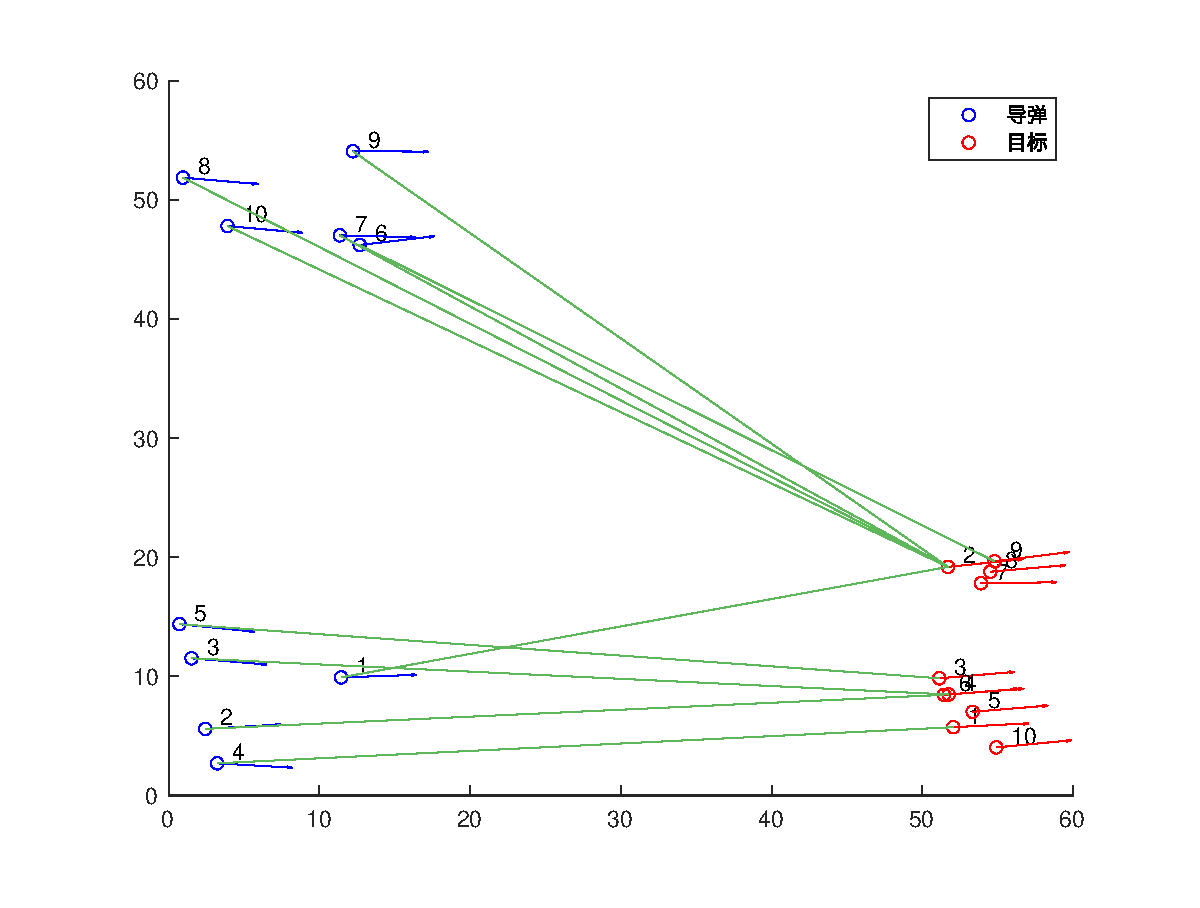
\includegraphics[height=5.5cm]{stochastic_game/HCG两集群0时刻}}
  \subcaptionbox{集群间建立通信}{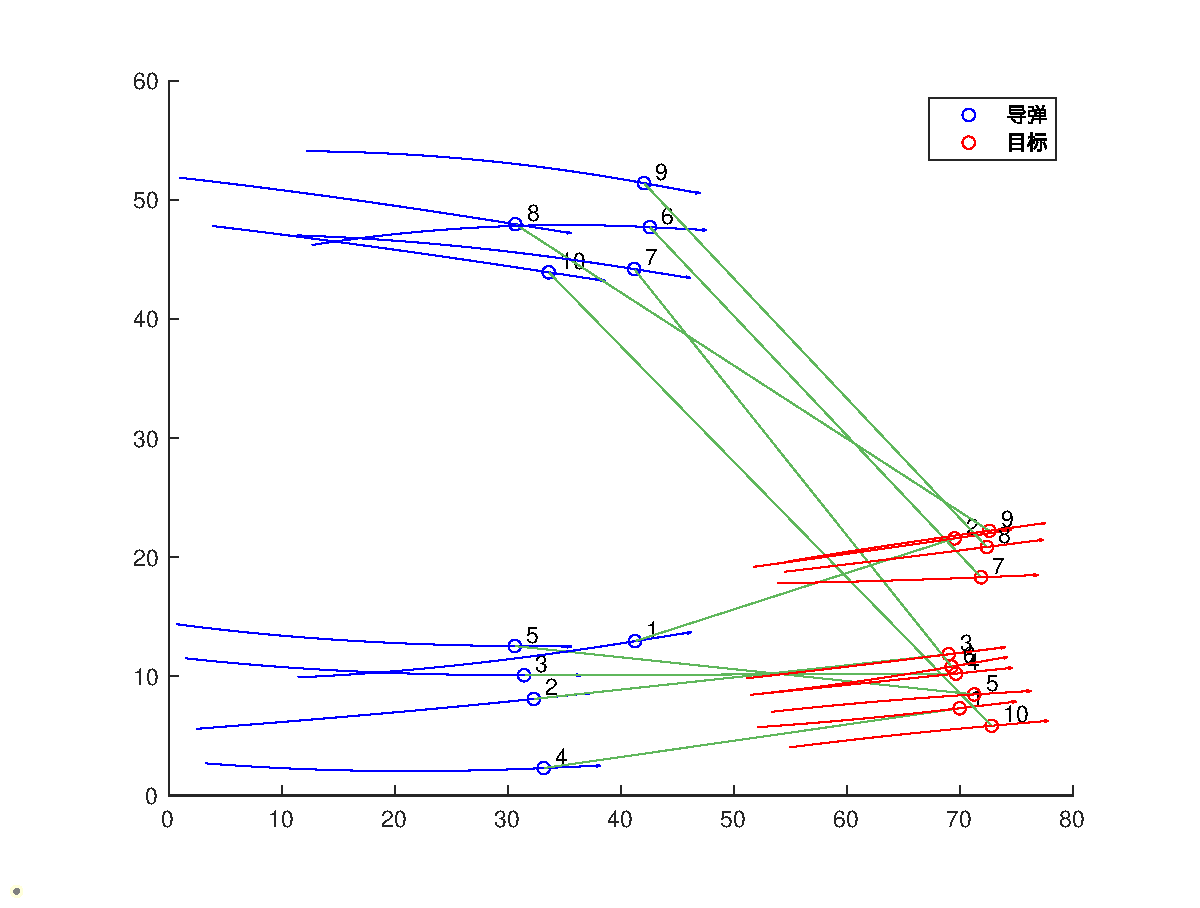
\includegraphics[height=5.5cm]{stochastic_game/HCG两集群1500时刻}}
  \subcaptionbox{攻击过程中后期}{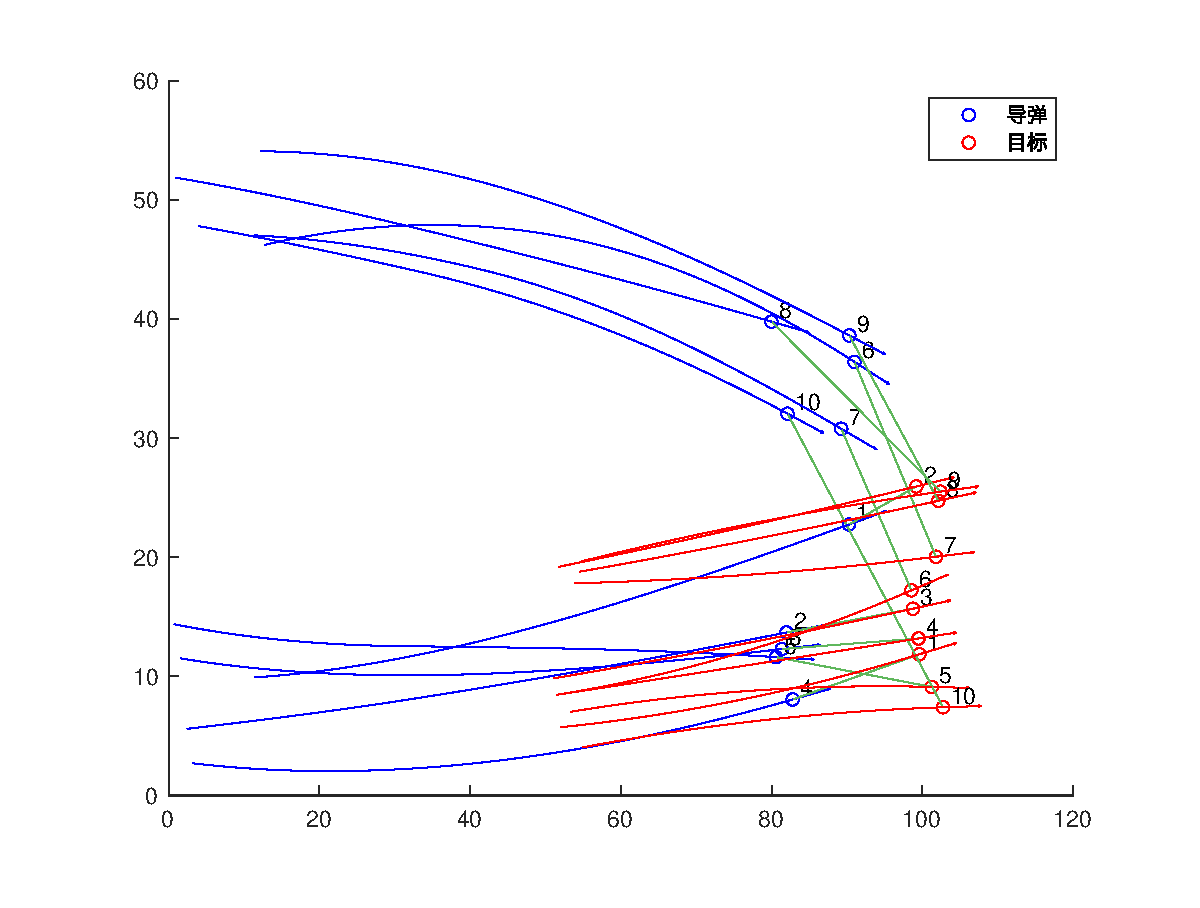
\includegraphics[height=5.5cm]{stochastic_game/HCG两集群4000时刻}}
  \subcaptionbox{攻击完成时刻}{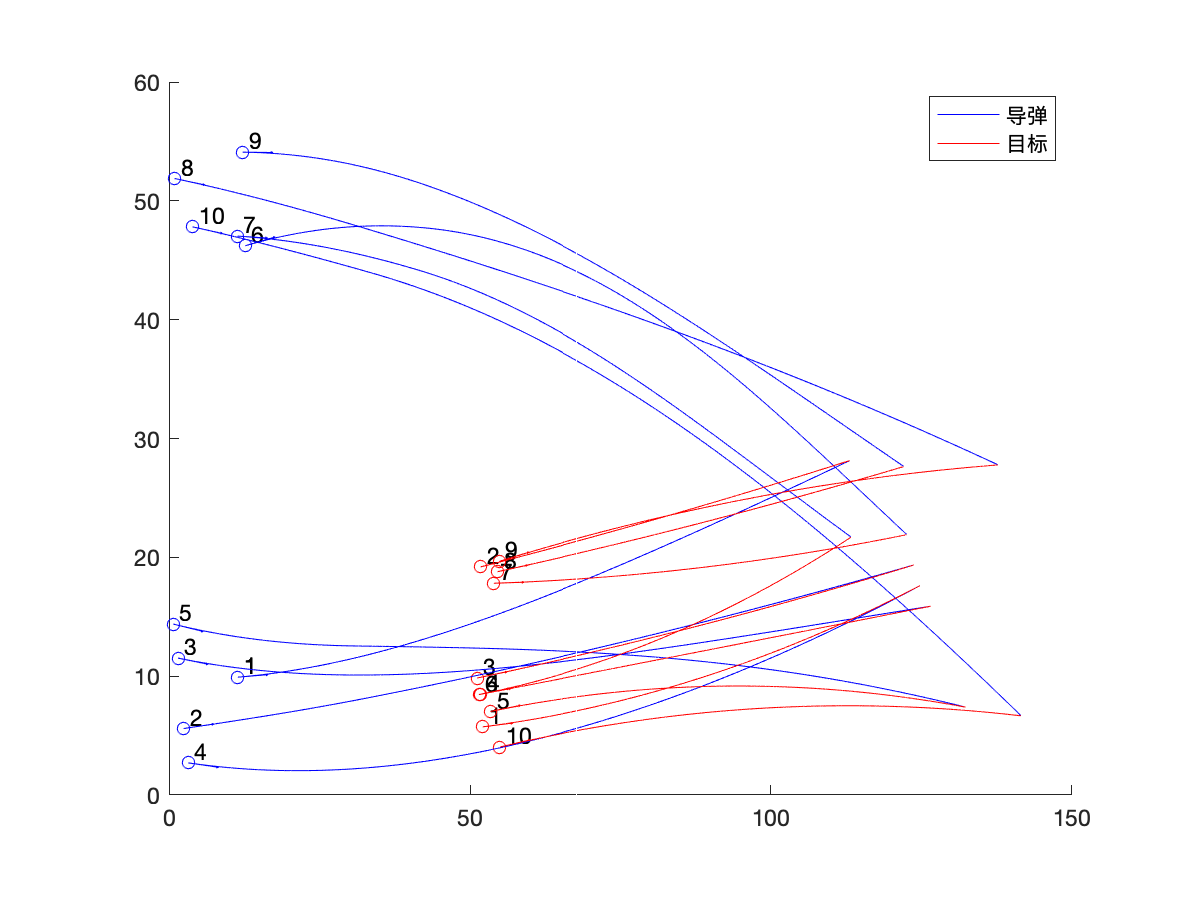
\includegraphics[height=5.5cm]{stochastic_game/HCG两集群最终}}
  \bicaption{导弹初始通信网络非连通的动态任务分配效果}
            {Dynamic task assignment in the scenario with disconnected initial communication network}
  \label{sg:fig:disconnected}
\end{figure}

(2)目标数量变化

在第一种非连通网络场景下,已经可以看出动态任务分配系统对于新增目标的响应机制,但为了更加直接地验证目标数量可变的场景下的系统动态响应能力,设置仿真场景中的部分目标初始位于导弹集群的探测范围外,因此事先导弹并不知道这些目标的存在,但随着攻击过程的进行,弹目间距离缩小,原本不被发现的目标将可能被发现,从而触发系统的重分配机制。

图\ref{sg:fig:newtarget}展示的是10vs10场景下出现新增目标的场景。在初始时刻,1-5号目标处于导弹集群的探测范围外,因此导弹初始分配方案如图\ref{sg:fig:newtarget}(a)所示,只在6-10号目标分配。由于导弹的速度远远大于目标,因此随着攻击过程的进行,原本在探测范围外的目标开始可以被导弹集群捕捉到,此时会触发重分配,增加了可选目标的导弹会重新选择目标,如图\ref{sg:fig:newtarget}(b)所示。

由于弹目距离的远近不同,一部分目标会率先被导弹击中,击中后的导弹与目标同时退出分配模型,剩下未完成攻击的导弹和未被击中的目标继续参与分配过程。如图\ref{sg:fig:newtarget}(c)所示,图中已经完成攻击的导弹与目标位置重叠,为了图示清晰不再画出轨迹,而其他还在攻击过程的导弹则对剩余目标重新分配,并继续飞行,直至所有目标均被击中,攻击完成,如图\ref{sg:fig:newtarget}(d)所示。

\begin{figure}[!hbtp]
  \centering
  \subcaptionbox{初始时刻}{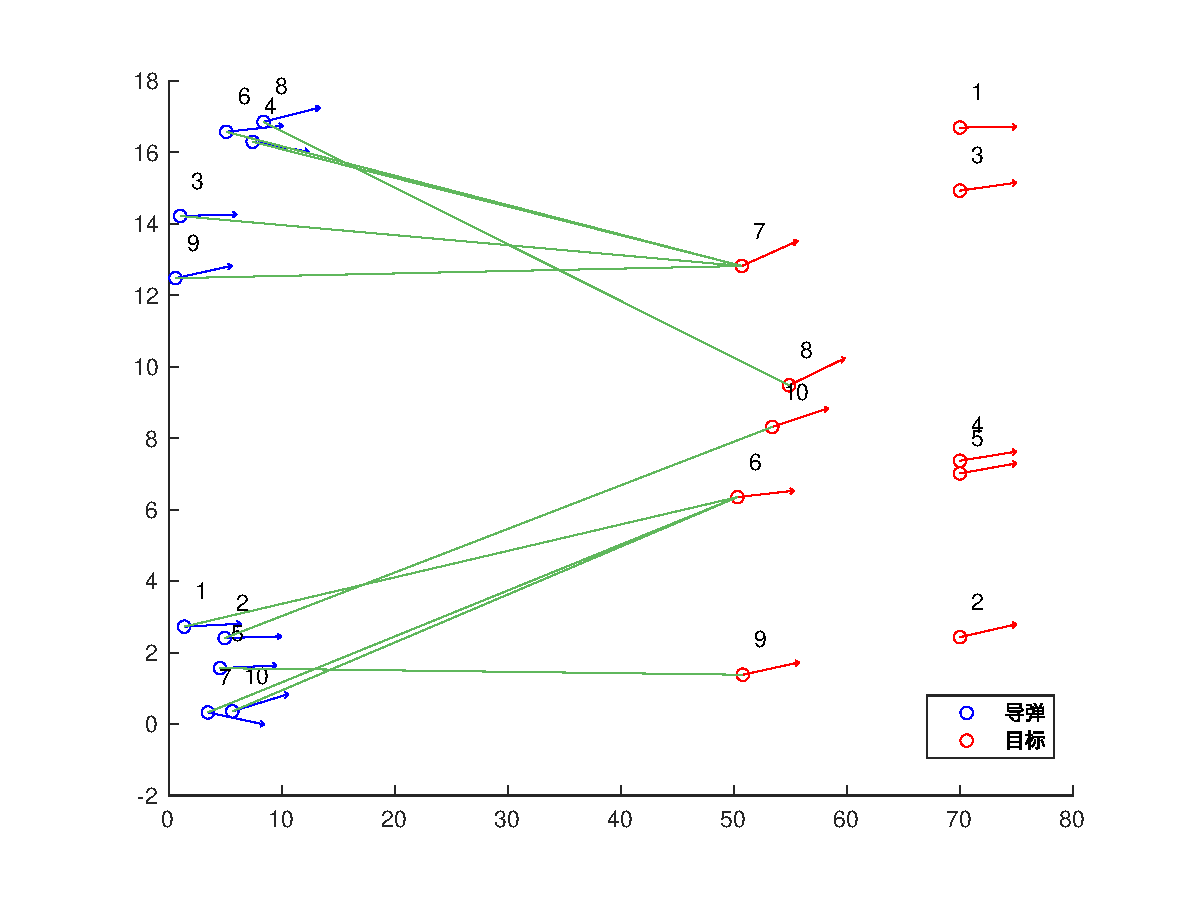
\includegraphics[height=5.5cm]{stochastic_game/HCG新增目标0时刻}}
  \subcaptionbox{发现新目标}{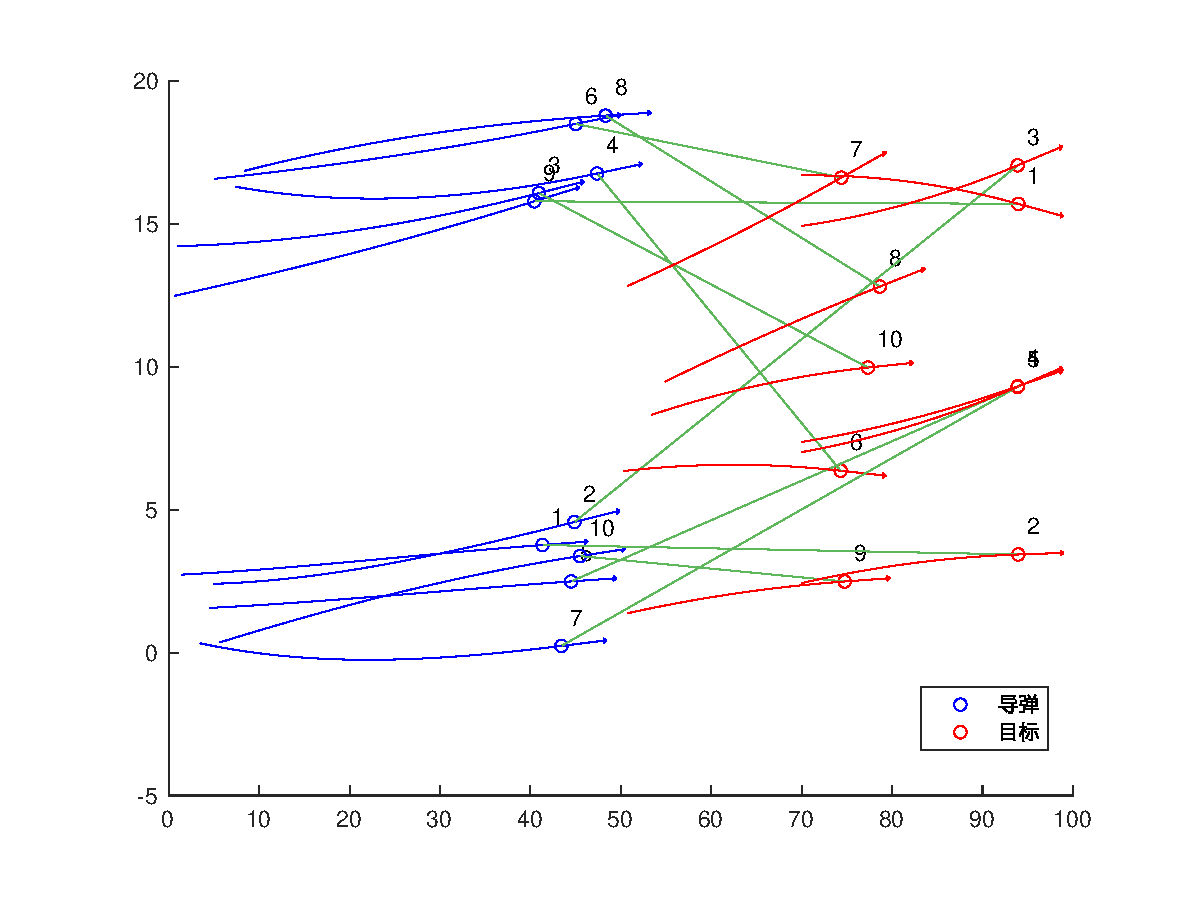
\includegraphics[height=5.5cm]{stochastic_game/HCG新增目标2000时刻}}
  \subcaptionbox{部分完成攻击}{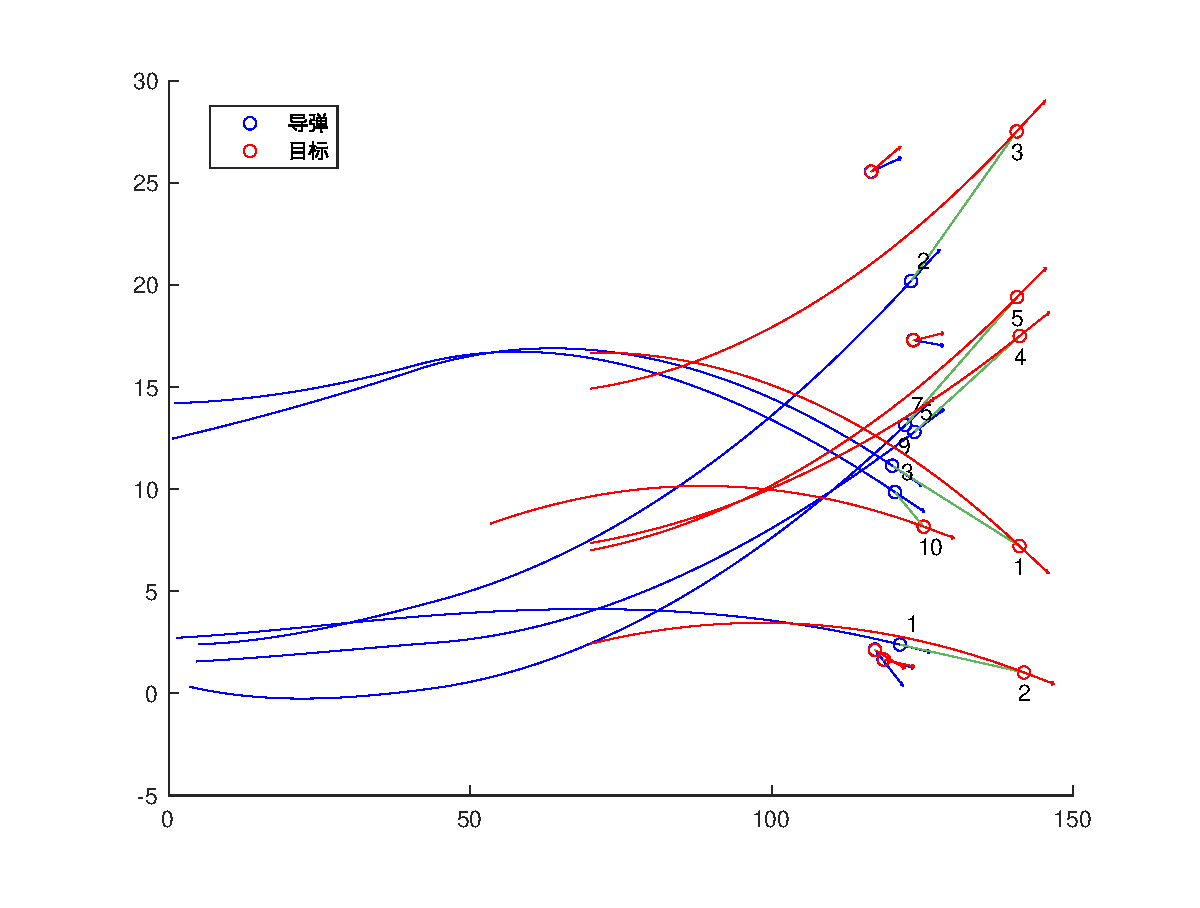
\includegraphics[height=5.5cm]{stochastic_game/HCG新增目标6000时刻}}
  \subcaptionbox{攻击完成时刻}{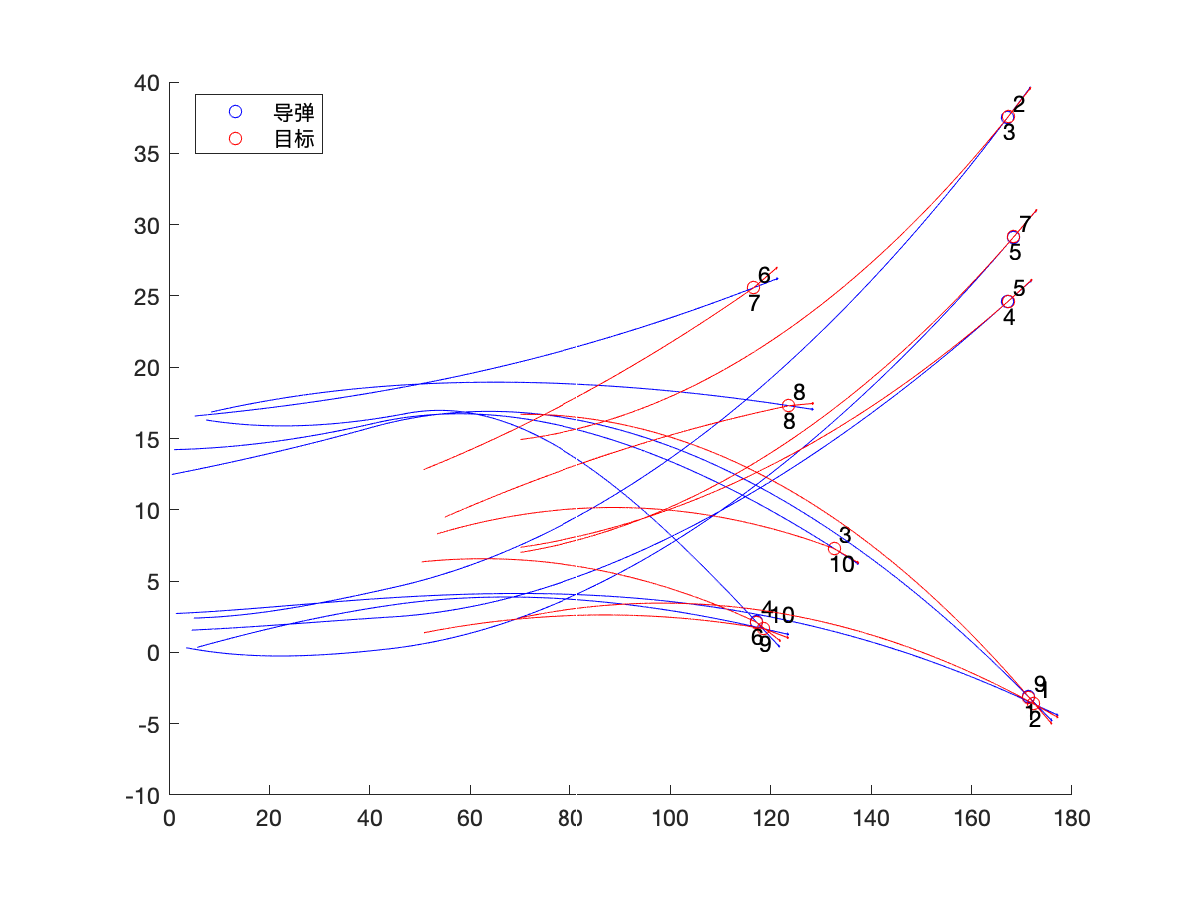
\includegraphics[height=5.5cm]{stochastic_game/HCG新增目标最终}}
  \bicaption{新增目标场景下的动态任务分配效果}
            {Dynamic task assignment in the scenario with new target appearance}
  \label{sg:fig:newtarget}
\end{figure}


通过以上仿真实验结果可以看出,本章基于随机博弈模型和任务重分配触发机制设计的动态任务分配系统对于非连通网络和目标数量可变两种非理想场景都具有较好的自适应性和动态响应能力,可以完成在较为复杂场景下的导弹集群动态任务分配。

\section{本章小结}
\label{reassign:sec:conclusion}

本章针对动态环境下的任务分配问题,基于随机博弈模型,将动态分配问题划分为若干时间窗口下的阶段性博弈模型,在每个博弈阶段使用势博弈或偏好联盟博弈建立任务分配模型求解。针对博弈阶段之间的切换,本章设计了阶段开始时的分配解变异机制和阶段结束时的分配解判别机制。由于实际场景中可能遇到新生事件或各种非理想情况,本文针对导弹通信网络非连通和目标数量变化这两种典型场景,各自分析了系统响应方案,并设计了任务重分配机制。最终本章给出了通过设计仿真场景进行实验,验证了本章设计的动态任务分配系统在非理想场景或新生事件下具有良好的适应能力。


% !TEX root = ../main.tex

\chapter{总结与展望}
\label{summary}

\section{本文总结}

随着集群技术的发展,在现代空战中,大规模集群空战是各个主要军事大国争夺的科技制高点。本文以空空导弹集群为研究目标,考虑了导弹的预计攻击时间和机动消耗能量,将未来的态势因素纳入模型考虑之中,建立了空空导弹任务分配模型。本文以博弈论为理论工具,使用势博弈模型、偏好联盟博弈模型研究了静态分布式任务分配方法,并以随机博弈模型为基础探讨了动态分布式任务分配的解决方案,取得了一些成果,本文的工作和主要贡献如下:

1. 针对分布式静态任务分配问题,本文基于势博弈模型理论设计了任务效用函数和基于WLU的智能体效用函数,针对现有使用势博弈模型解决任务分配问题的文献大多没有考虑含约束分配问题,本文引入Lagrange乘子对WLU效用函数进行修正,并从理论上证明了修正后的WLU效用函数的可行性,推导出了使用修正WLU效用函数的势博弈模型的性能下界。接着,结合现有文献成果,本文介绍了三种博弈学习算法:JSFP、GRMFMI和SAP算法,并针对博弈学习算法容易过早收敛,陷入局部最优的问题,在SAP算法的基础上设计了任务交易机制,提出了含任务交易的SAP算法。通过与几种集中式启发算法的对比仿真验证,结果表明本文设计的模型与算法在平衡分配问题和非平衡分配问题上都具有良好的效果,且相比集中式算法在较大规模问题上更具时间优势。

2. 将静态任务分配问题看作联盟形成问题,本文基于偏好联盟博弈理论建立了任务分配模型。在偏好联盟博弈模型中,引入智能体对联盟的偏好关系,并假设智能体对联盟的偏好仅与联盟成员数量有关,而与具体成员无关,并从理论上证明当智能体偏好关系满足社交疏远性质时,偏好联盟博弈模型一定存在纳什均衡。本文根据以上结论设计了边际效用递减的任务效用函数和满足社交疏远性质的智能体效用函数,并针对具体函数推导出偏好联盟博弈模型的性能下界。针对博弈学习算法,本文除了使用势博弈模型中的带任务交易的SAP算法外,还介绍了一种分布式一致算法DMCA,用于实现分布式架构下的联盟形成问题。通过设计仿真试验,本文对比分析了非平衡分配问题中两种非平衡程度对于学习算法的性能影响,结果表明本文提出的两种博弈模型下的五种学习算法在非平衡问题中具有良好的求解能力,并且有着良好的实时性。

3. 针对动态任务分配模型,本文基于随机博弈理论,将动态任务分配模型分解为若干时间窗口下的静态博弈阶段,在每个阶段博弈中建立势博弈或偏好联盟博弈模型并求解。针对博弈阶段之间的切换问题,设计了初始分配生成机制和分配传递机制,以保证在满足动态要求的前提下,保持分配的稳定性和可行性。针对动态环境中可能出现的非理想情况,本文针对非连通场景和目标数量变化两种场景设计了重分配触发机制,分析了非连通情况下可以触发重分配和消解分配冲突的条件,并针对几种目标数量变化的场景下的重分配进行了分析。本文建立了完整的分布式动态任务分配系统,并通过仿真实验验证了该系统的有效性,并设计了几种非理想情况下的重分配场景,验证了系统在突发事件下具有良好的动态自适应性。

\section{未来展望}

本文基于博弈论的思想对空空导弹的分布式任务分配模型和算法进行了相关研究,但实际场景中大规模多对多空战场景要更为复杂,分配难度也更大,且本文提出的模型和算法也存在着一些局限与问题还需要进一步的研究。下一步工作主要包括以下几个方面:

1. 动态任务分配环境的建模问题。本文建立的任务分配问题模型是基于导弹预计剩余攻击时间和预计机动能量,虽然一定程度上考虑了未来的因素,但实际模型更加复杂,包括导弹集群的路径规划、目标机动、导弹和目标的运动特性等因素对分配的影响尚未考虑在内。如何选取对任务分配有影响的因素,并处理这些因素的动态变化对分配的影响,结合导弹与目标的运动规律,建立更符合实际的任务分配模型是一个仍待解决的问题。

2. 算法的精确度和普适性问题。基于博弈论的任务分配模型和算法可以在较快时间内获得较为精确的解,但受限于模型的设置,这类算法往往比集中式算法更容易陷入局部最优中,因此也导致了求解结果较为分散的问题,。针对以上问题,本文虽然提出了一些解决思路,但并没有完全解决。此外,基于博弈论的分配模型受限于模型函数和参数的设计,设计不当可能会使得模型在某些场景下失效,本文针对模型的设计和参数的选择范围进行了初步探究,但这个问题仍需更多的工作。

3. 动态任务重分配机制设计问题。本文只研究了通信网络非连通和目标数量变化两种场景下的重分配问题,但实际动态场景中,需要进行重分配的事件更多更复杂,比如导弹发生故障、目标突然丢失等等;此外,当重分配事件增多时,如何协调这些事件的优先级和处理方式本文没有深入展开研究。


%TC:ignore

% 使用英文字母对附录编号

% 附录内容

% 后文部分无编号
\backmatter

% 参考文献
\printbibliography[heading=bibintoc]

% 用于盲审的论文需隐去致谢、发表论文、科研成果、简历

% 致谢
% !TEX root = ../main.tex

\begin{acknowledgements}
  感谢那位最先制作出博士学位论文 \LaTeX 模板的交大物理系同学!

  感谢 William Wang 同学对模板移植做出的巨大贡献!

  感谢 \href{https://github.com/weijianwen}{@weijianwen} 学长一直以来的开发和维
  护工作!

  感谢 \href{https://github.com/sjtug}{@sjtug} 以及
   \href{https://github.com/dyweb}{@dyweb} 对 0.9.5 之后版本的开发和维护工作!

  感谢所有为模板贡献过代码的同学们, 以及所有测试和使用模板的各位同学!

  感谢 \LaTeX 和 \href{https://github.com/sjtug/SJTUThesis}{\sjtuthesis},帮我节
  省了不少时间。
\end{acknowledgements}


% 发表论文、科研成果、简历
% 盲审论文中,发表论文及科研成果等仅以第几作者注明即可,不要出现作者或他人姓名
% !TEX root = ../main.tex

\begin{publications}
  \item Chen H, Chan C~T. Acoustic cloaking in three dimensions using acoustic metamaterials[J]. Applied Physics Letters, 2007, 91:183518.
  \item Chen H, Wu B~I, Zhang B, et al. Electromagnetic Wave Interactions with a Metamaterial Cloak[J]. Physical Review Letters, 2007, 99(6):63903.
\end{publications}

\begin{publications*}
  \item 第一作者. 中文核心期刊论文, 2007.
  \item 第一作者. EI 国际会议论文, 2006.
\end{publications*}

% !TEX root = ../main.tex

\begin{achievements}
  \item 第一发明人,“永动机”,专利申请号202510149890.0
\end{achievements}

\begin{achievements*}
  \item 第一发明人,“永动机”,专利申请号XXXXXXXXXXXX.X
\end{achievements*}

%% !TEX root = ../main.tex

\begin{resume}
  \subsection*{基本情况}
    某某,yyyy 年 mm 月生于 xxxx。

  \subsection*{教育背景}
  \begin{itemize}
    \item yyyy 年 mm 月至今,上海交通大学,博士研究生,xx 专业
    \item yyyy 年 mm 月至 yyyy 年 mm 月,上海交通大学,硕士研究生,xx 专业
    \item yyyy 年 mm 月至 yyyy 年 mm 月,上海交通大学,本科,xx 专业
  \end{itemize}

  \subsection*{研究兴趣}
    \LaTeX{} 排版

  \subsection*{联系方式}
  \begin{itemize}
    \item 地址: 上海市闵行区东川路 800 号,200240
    \item E-mail: \email{xxx@sjtu.edu.cn}
  \end{itemize}
\end{resume}


% 中文学士学位论文要求在最后有一个英文大摘要,单独编页码,英文学士学位论文不需要
% !TEX root = ../main.tex

\begin{digest}
  An imperial edict issued in 1896 by Emperor Guangxu, established Nanyang
  Public School in Shanghai. The normal school, school of foreign studies,
  middle school and a high school were established. Sheng Xuanhuai, the person
  responsible for proposing the idea to the emperor, became the first president
  and is regarded as the founder of the university.

  During the 1930s, the university gained a reputation of nurturing top
  engineers. After the foundation of People's Republic, some faculties were
  transferred to other universities. A significant amount of its faculty were
  sent in 1956, by the national government, to Xi'an to help build up Xi'an Jiao
  Tong University in western China. Afterwards, the school was officially
  renamed Shanghai Jiao Tong University.

  Since the reform and opening up policy in China, SJTU has taken the lead in
  management reform of institutions for higher education, regaining its vigor
  and vitality with an unprecedented momentum of growth. SJTU includes five
  beautiful campuses, Xuhui, Minhang, Luwan Qibao, and Fahua, taking up an area
  of about 3,225,833 m2. A number of disciplines have been advancing towards the
  top echelon internationally, and a batch of burgeoning branches of learning
  have taken an important position domestically.

  Today SJTU has 31 schools (departments), 63 undergraduate programs, 250
  masters-degree programs, 203 Ph.D. programs, 28 post-doctorate programs, and
  11 state key laboratories and national engineering research centers.

  SJTU boasts a large number of famous scientists and professors, including 35
  academics of the Academy of Sciences and Academy of Engineering, 95 accredited
  professors and chair professors of the "Cheung Kong Scholars Program" and more
  than 2,000 professors and associate professors.

  Its total enrollment of students amounts to 35,929, of which 1,564 are
  international students. There are 16,802 undergraduates, and 17,563 masters
  and Ph.D. candidates. After more than a century of operation, Jiao Tong
  University has inherited the old tradition of "high starting points, solid
  foundation, strict requirements and extensive practice." Students from SJTU
  have won top prizes in various competitions, including ACM International
  Collegiate Programming Contest, International Mathematical Contest in Modeling
  and Electronics Design Contests. Famous alumni include Jiang Zemin, Lu Dingyi,
  Ding Guangen, Wang Daohan, Qian Xuesen, Wu Wenjun, Zou Taofen, Mao Yisheng,
  Cai Er, Huang Yanpei, Shao Lizi, Wang An and many more. More than 200 of the
  academics of the Chinese Academy of Sciences and Chinese Academy of
  Engineering are alumni of Jiao Tong University.
\end{digest}


%TC:endignore

\end{document}
